\chapter{Analisi sperimentale}
\label{cha:NTPsec} \label{cha:NTPsec}

Il presente capitolo è dedicato all’analisi dei dati raccolti per i demoni
\texttt{\textbf{NTPsec}}, \texttt{\textbf{ptp4l}}, \texttt{\textbf{Chronyd}} con l’obiettivo
di valutarne il comportamento al variare delle condizioni di rete introdotte nei tre
scenari sperimentali. L’attenzione è rivolta all’esame delle principali metriche
di sincronizzazione temporale osservate durante la fase di testing, al fine di evidenziare
l’eventuale impatto del progressivo incremento degli impairment di rete sulla stabilità
del sistema e sulla qualità del processo di sincronizzazione.

L’analisi è organizzata per metrica. Per ciascuna grandezza considerata viene
condotto un confronto sistematico tra i tre scenari sperimentali definiti in
precedenza, corrispondenti a differenti livelli di degrado della rete (\texttt{low},
\texttt{medium}, \texttt{high}). Tale confronto si basa sull’osservazione dei dati
raccolti e sulla loro rappresentazione grafica, con lo scopo di mettere in
evidenza eventuali variazioni nel comportamento del demone in termini di
accuratezza della sincronizzazione, variabilità delle misurazioni e dinamica di convergenza.

\begin{table}[H]
  \centering
  \caption{Matrice di scenario - fase 3 (topologia T2 + tc/netem)}
  \begin{tabular}{|c|c|c|c|c|c|}
    \hline
    \textbf{Scenario} & \textbf{Delay} & \textbf{Jitter} & \textbf{Loss} & \textbf{Reorder} & \textbf{Rate Limit} \\
    \hline
    LOW               & 5 ms           & 1 ms            & 0.1\%         & 1\%              & 50 Mbit             \\
    \hline
    MEDIUM            & 15 ms          & 5 ms            & 0.5\%         & 5\%              & 20 Mbit             \\
    \hline
    HIGH              & 60 ms          & 20 ms           & 10\%          & 20\%             & 5 Mbit              \\
    \hline
  \end{tabular}
  \label{tab:scenario_matrix}
\end{table}
\section{\texttt{NTPsec}}

Nel caso di \texttt{\textbf{NTPsec}}, l’analisi si concentra su tre metriche
principali: \texttt{\textbf{delay}}, \texttt{\textbf{jitter}} e \texttt{\textbf{offset}}.
Tali grandezze consentono di caratterizzare, rispettivamente, il tempo di
propagazione dei pacchetti NTP, la variabilità temporale delle misurazioni e lo scostamento
tra il clock locale e il clock di riferimento. La loro evoluzione nei diversi
scenari permette quindi di valutare la robustezza del demone rispetto al degrado
delle condizioni di rete e di analizzare la qualità del processo di
sincronizzazione in termini sia di stabilità sia di accuratezza.

I dati oggetto dell’analisi sono stati raccolti secondo la metodologia
sperimentale illustrata nei capitoli precedenti. In questa sede, pertanto, non vengono
ripresi gli aspetti relativi alla configurazione dell’ambiente di prova o alla disposizione
della topologia, ma si assume come riferimento l’insieme delle misurazioni già
ottenute per ciascuna metrica e per ciascuno scenario di rete. Nel caso specifico
di \texttt{\textbf{NTPsec}}, le misurazioni considerate sono state rilevate sui nodi
\texttt{clientntp} e \texttt{boundary} della topologia, in coerenza con il ruolo
da essi ricoperto nel processo di sincronizzazione.

Ciascuna sezione seguente è quindi dedicata a una singola metrica e presenta, per
i tre scenari sperimentali, i risultati osservati e il relativo confronto
interpretativo, con l’obiettivo di individuare eventuali differenze significative
tra le condizioni di rete considerate e valutarne gli effetti sul comportamento del
demone.

\subsection{\texttt{clientntp}}
L'analisi condotta sul nodo \texttt{clientntp} è caratterizzata da uno stato di
inizializzazione, identificato da \texttt{refid=.INIT.}, \texttt{stratum=16}, \texttt{selected=False}
e \texttt{reach=0}. Tale intervallo non rappresenta il regime operativo della
sincronizzazione e non viene quindi considerato nel confronto tra scenari, che viene
invece condotto a partire dal primo campione valido, corrispondente in tutti i
casi a +450 secondi di tempo relativo.
\subsubsection{Analisi metrica: \texttt{delay}}
\begin{figure}[H]
  \centering

  \begin{subfigure}
    {0.32\textwidth}
    \centering
    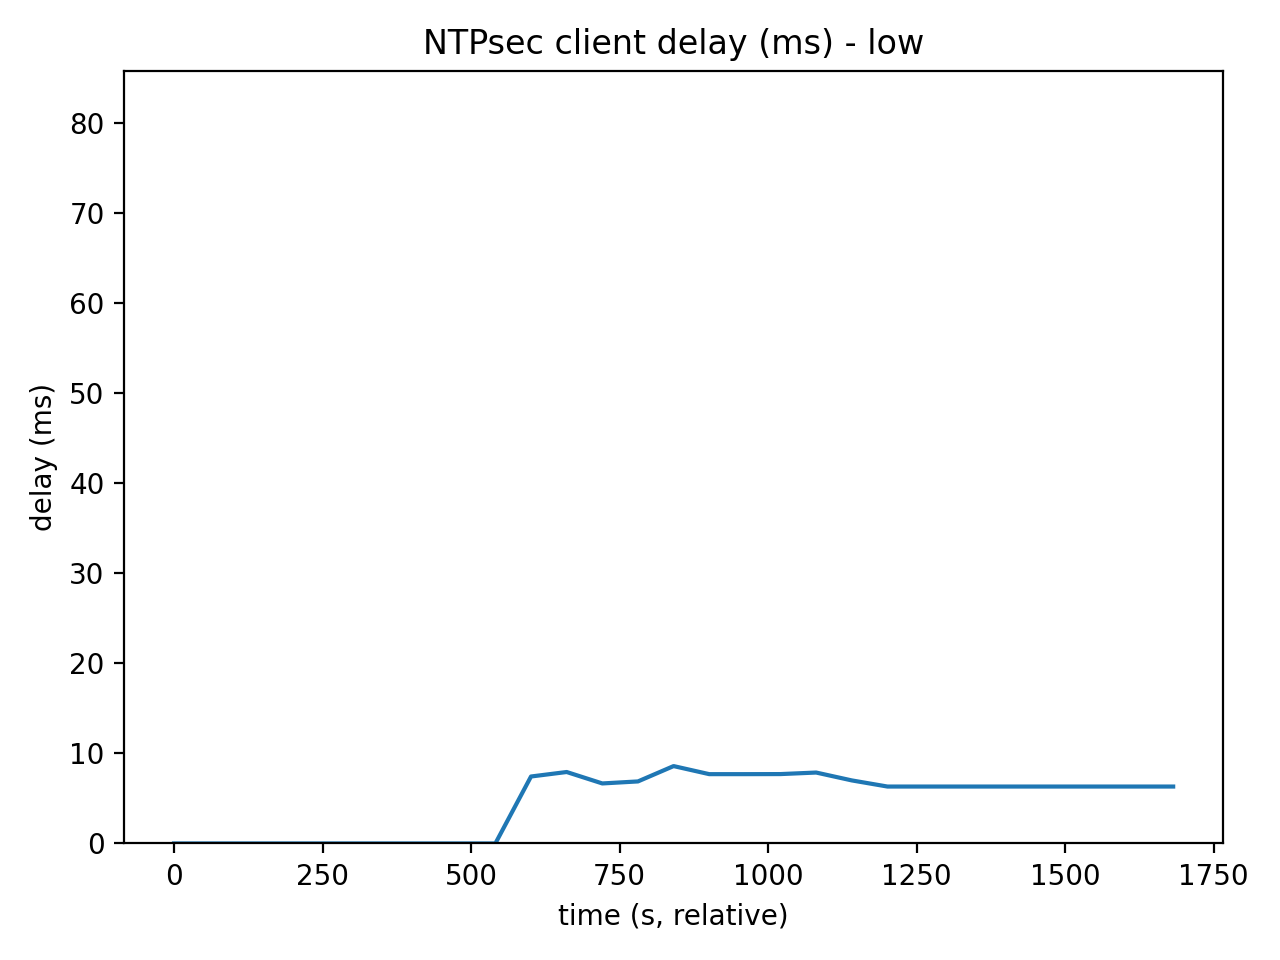
\includegraphics[width=\linewidth]{
      images/data_plots/plots_ntpsec/ntpsec_client_low_delay_ms.png
    }
    \caption{Scenario LOW}
  \end{subfigure}
  \hfill
  \begin{subfigure}
    {0.32\textwidth}
    \centering
    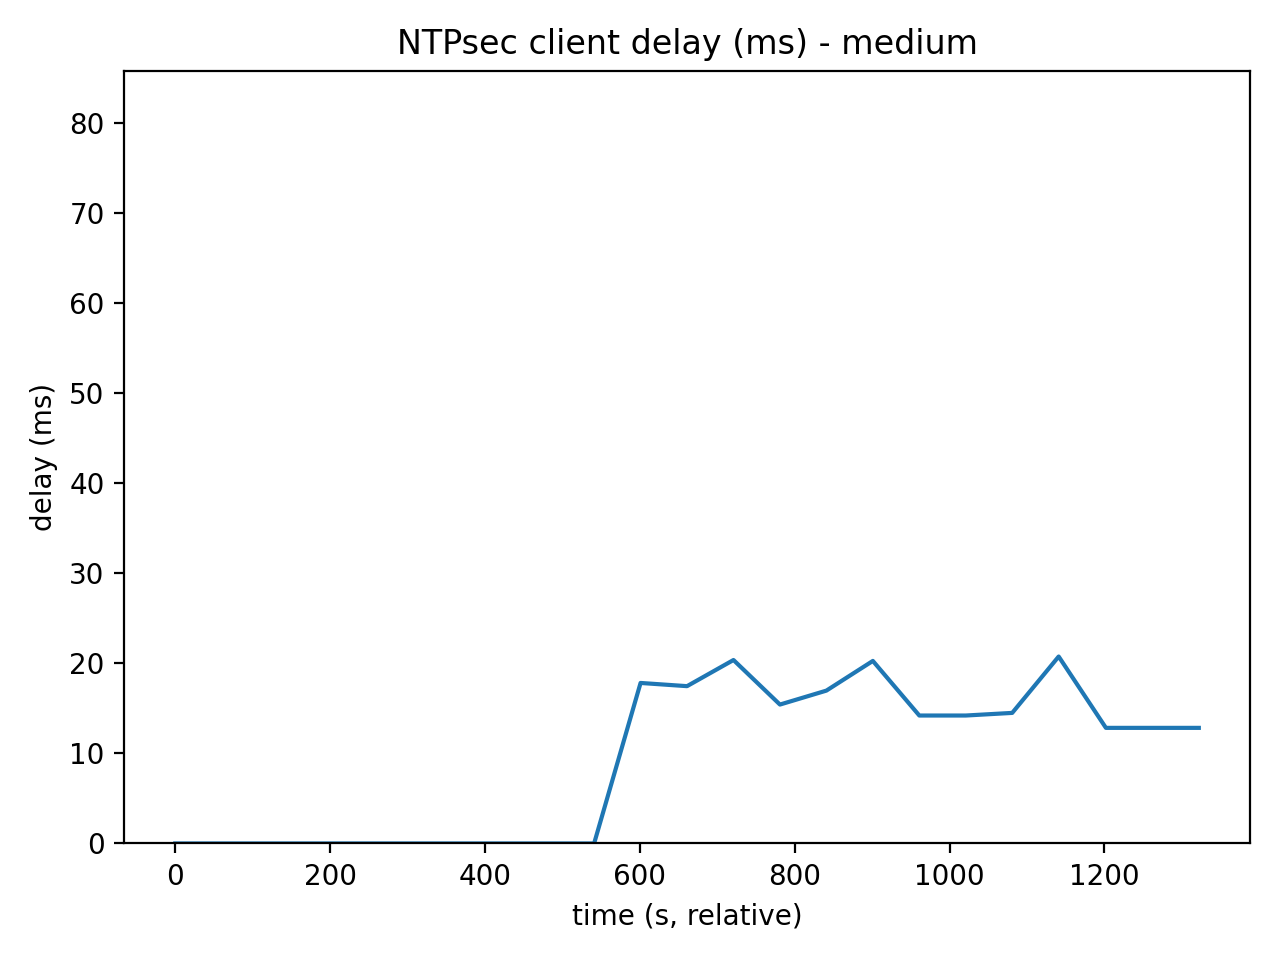
\includegraphics[width=\linewidth]{
      images/data_plots/plots_ntpsec/ntpsec_client_medium_delay_ms.png
    }
    \caption{Scenario MEDIUM}
  \end{subfigure}
  \hfill
  \begin{subfigure}
    {0.32\textwidth}
    \centering
    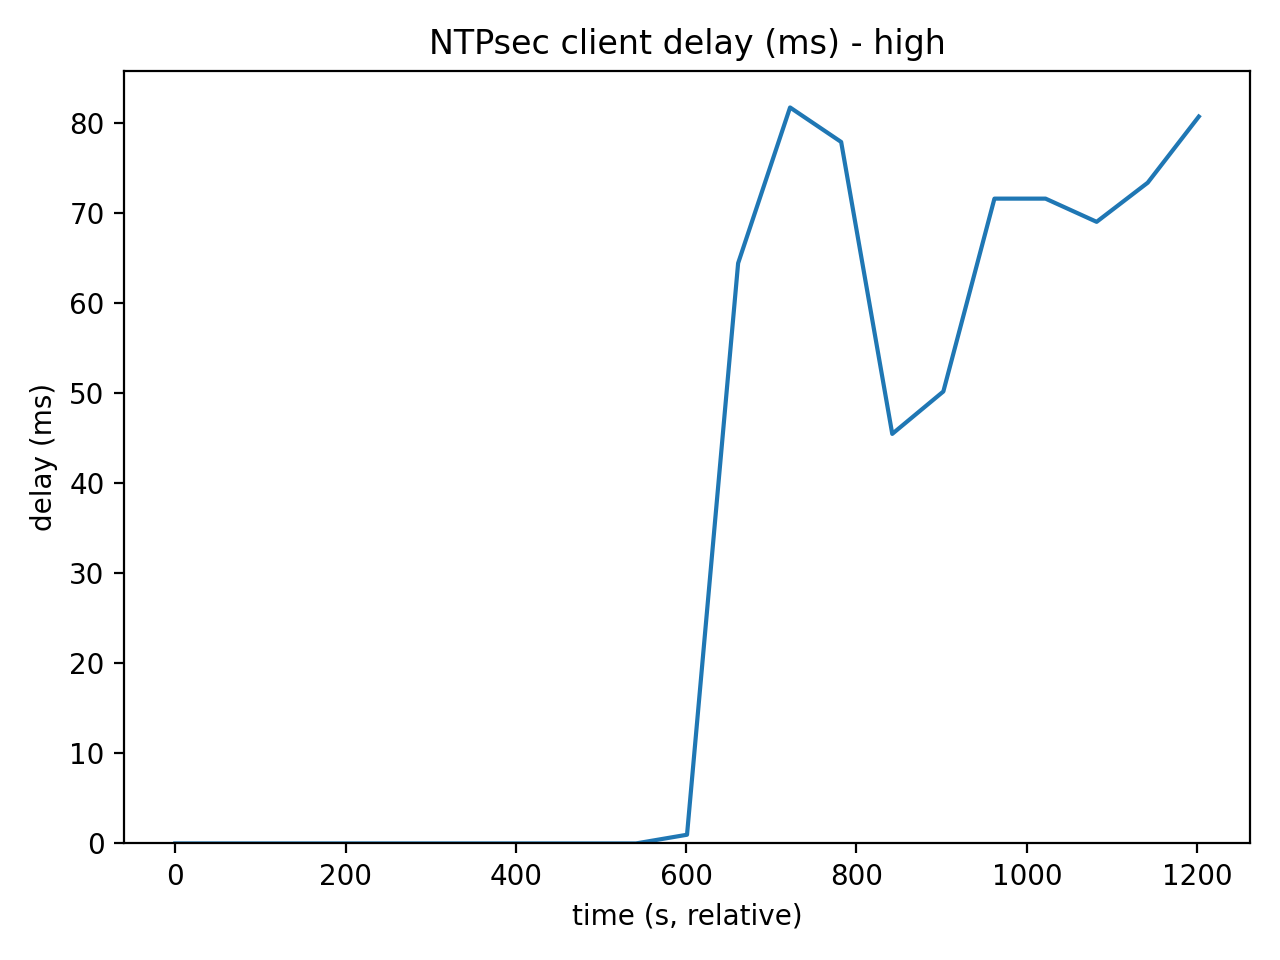
\includegraphics[width=\linewidth]{
      images/data_plots/plots_ntpsec/ntpsec_client_high_delay_ms.png
    }
    \caption{Scenario HIGH}
  \end{subfigure}

  \caption{Comparazione della performance - nodo: \texttt{clientntp}}
  \label{fig:scenario_comparison}
\end{figure}

L’analisi del \texttt{\textbf{delay}} misurato sul nodo \texttt{clientntp} per il
demone \texttt{\textbf{NTPsec}} evidenzia una dipendenza marcata dal livello di
impairment introdotto nei tre scenari sperimentali. Il risultato mette in evidenzia
un consistente e progressivo degrado al crescere della severità dello scenario di
rete. Si evidenzia un marcato incremento dia del livello della metrica sia della
sua dispersione.

Nello scenario \texttt{low}, il delay assume valori contenuti e presenta un
andamento fortemente regolare. Sui campioni validi si osserva un valore medio pari
a 6.96 ms, con deviazione standard di 0.75 ms, minimo di 6.32 ms e massimo di 8.59
ms. Il range complessivo risulta quindi pari a 2.27 ms. La serie mostra oscillazioni
modeste e una progressiva stabilizzazione su valori prossimi a 6.3 ms, indicando
che, in presenza di impairment ridotti, il percorso di rete mantiene
caratteristiche sufficientemente stabili da non introdurre ritardi significativi
né elevata variabilità nelle misure.

Nel caso \texttt{medium}, il delay cresce in modo netto e si colloca su una
fascia di valori sensibilmente superiore. La media dei campioni validi è pari a 16.18
ms, con deviazione standard di 2.96 ms, minimo di 12.83 ms e massimo di 20.75 ms.
Rispetto allo scenario \texttt{low}, il delay medio risulta quindi più che
raddoppiato, mentre aumentano in modo evidente anche la dispersione e l’ampiezza delle
oscillazioni. L’andamento della serie resta leggibile e non mostra fenomeni di
divergenza, ma la misura risulta meno regolare e più sensibile alla variabilità introdotta
dalla rete.

Lo scenario \texttt{high} presenta il comportamento più degradato. Al netto del primo
campione selezionato, che assume carattere transitorio rispetto al resto della
serie, il delay si colloca stabilmente in una fascia elevata, con media pari a
68.57 ms, deviazione standard di 12.18 ms, minimo di 45.46 ms e massimo di 81.69
ms. Il confronto con gli altri scenari evidenzia un incremento molto marcato: il
delay medio risulta circa 4.2 volte superiore rispetto al caso \texttt{medium} e circa
9.8 volte superiore rispetto al caso \texttt{low}. In questo scenario, oltre al
forte aumento del livello medio, si osserva anche una variabilità significativamente
maggiore, indice di una condizione di rete fortemente instabile dal punto di
vista temporale.

Nel complesso, il confronto tra i tre scenari mostra una progressione monotona del
delay al crescere della severità degli impairment di rete. Il passaggio da
\texttt{low} a \texttt{medium} comporta un incremento sensibile ma ancora
compatibile con un regime relativamente stabile; il passaggio da \texttt{medium}
a \texttt{high} introduce invece un cambiamento di regime molto più marcato, in
cui il ritardo osservato dal clientntp cresce drasticamente e la misura perde
gran parte della propria regolarità. La metrica del delay risulta pertanto particolarmente
efficace nel mettere in evidenza l’impatto del degrado della rete sul comportamento
del clientntp NTPsec.

\subsubsection{Analisi metrica: \texttt{jitter}}
\begin{figure}[H]
  \centering

  \begin{subfigure}
    {0.32\textwidth}
    \centering
    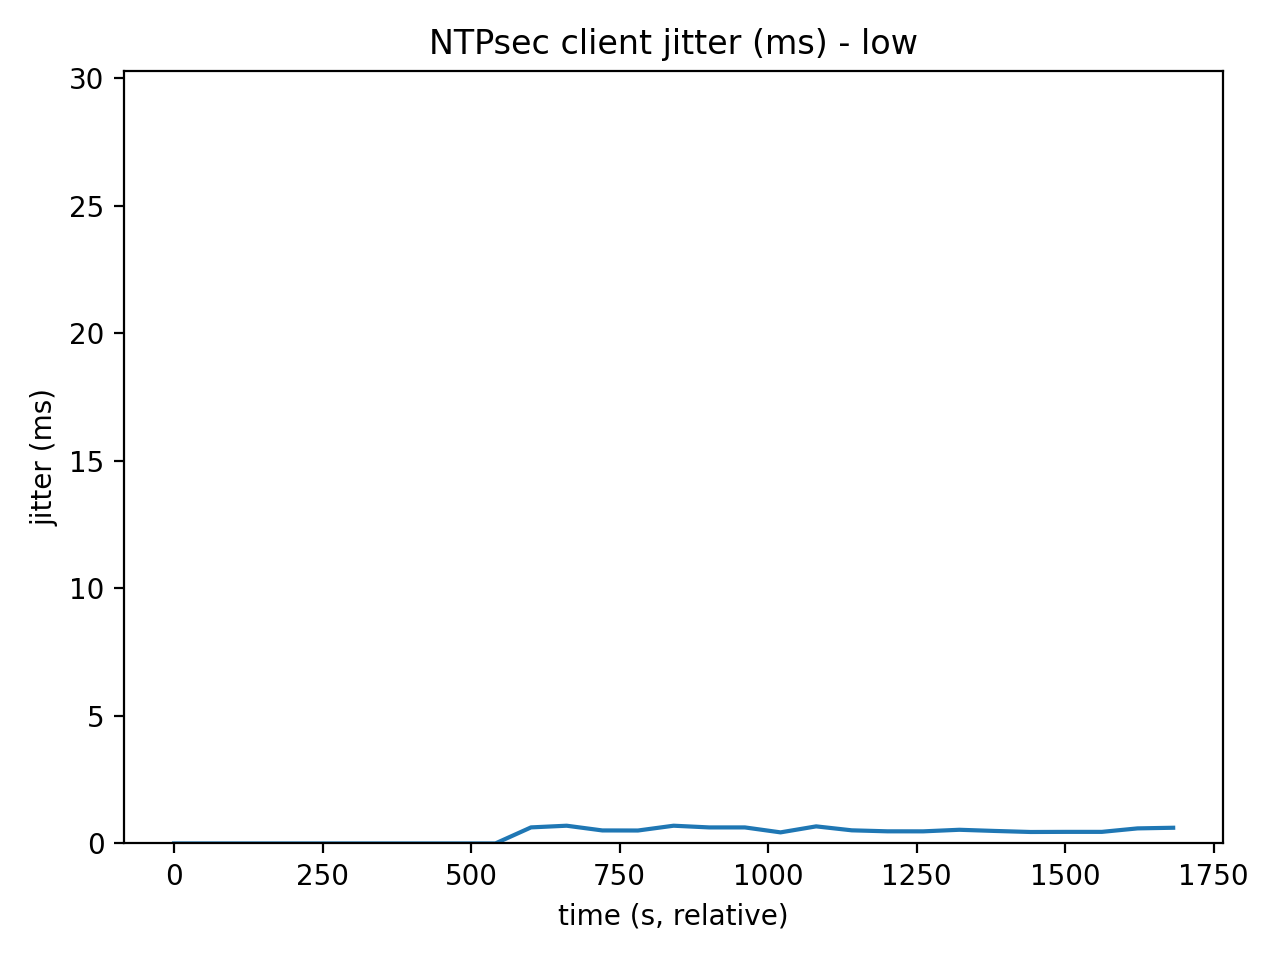
\includegraphics[width=\linewidth]{
      images/data_plots/plots_ntpsec/ntpsec_client_low_jitter_ms.png
    }
    \caption{Scenario LOW}
  \end{subfigure}
  \hfill
  \begin{subfigure}
    {0.32\textwidth}
    \centering
    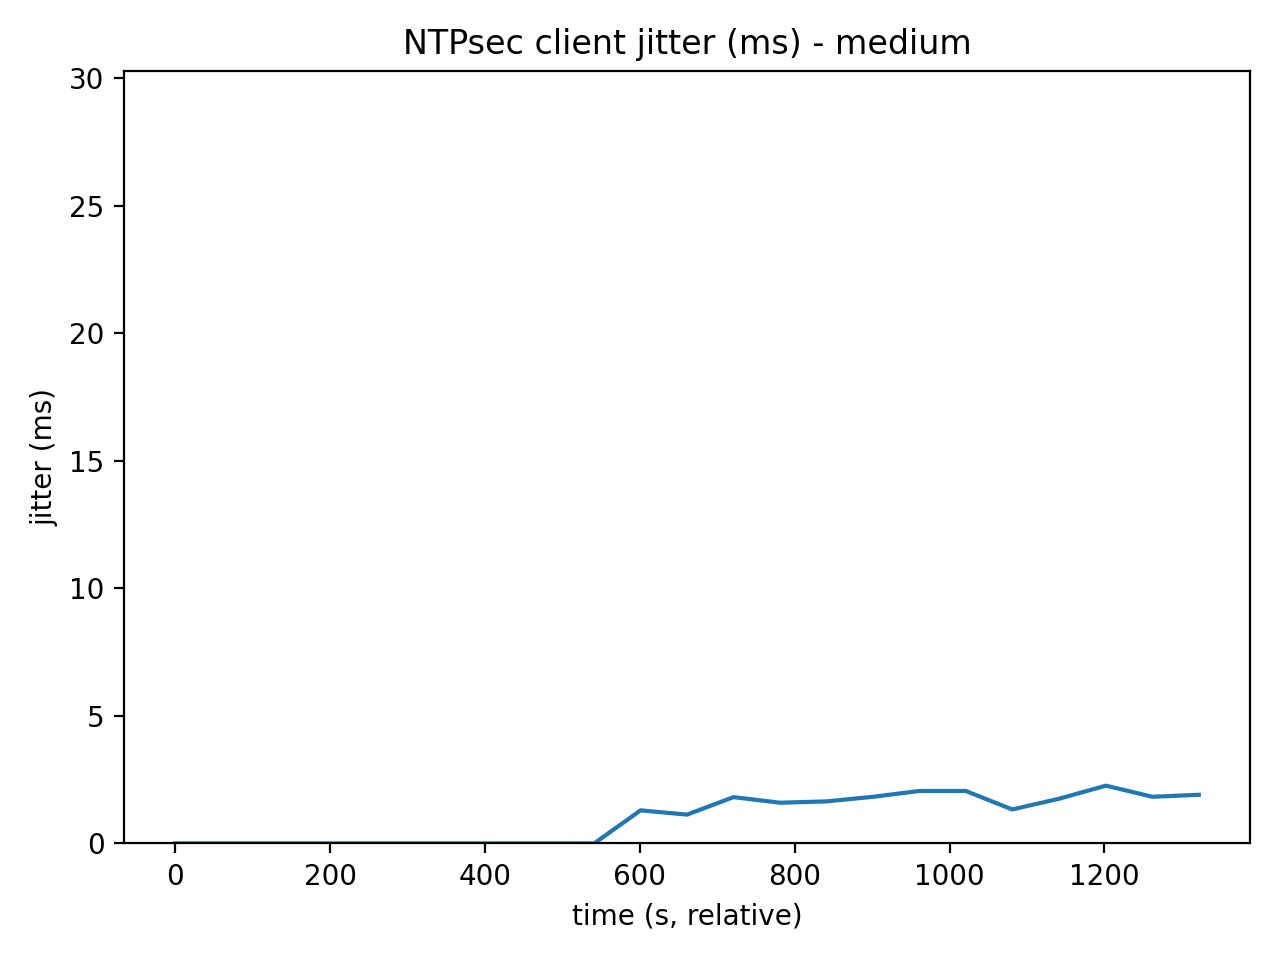
\includegraphics[width=\linewidth]{
      images/data_plots/plots_ntpsec/ntpsec_client_medium_jitter_ms.png
    }
    \caption{Scenario MEDIUM}
  \end{subfigure}
  \hfill
  \begin{subfigure}
    {0.32\textwidth}
    \centering
    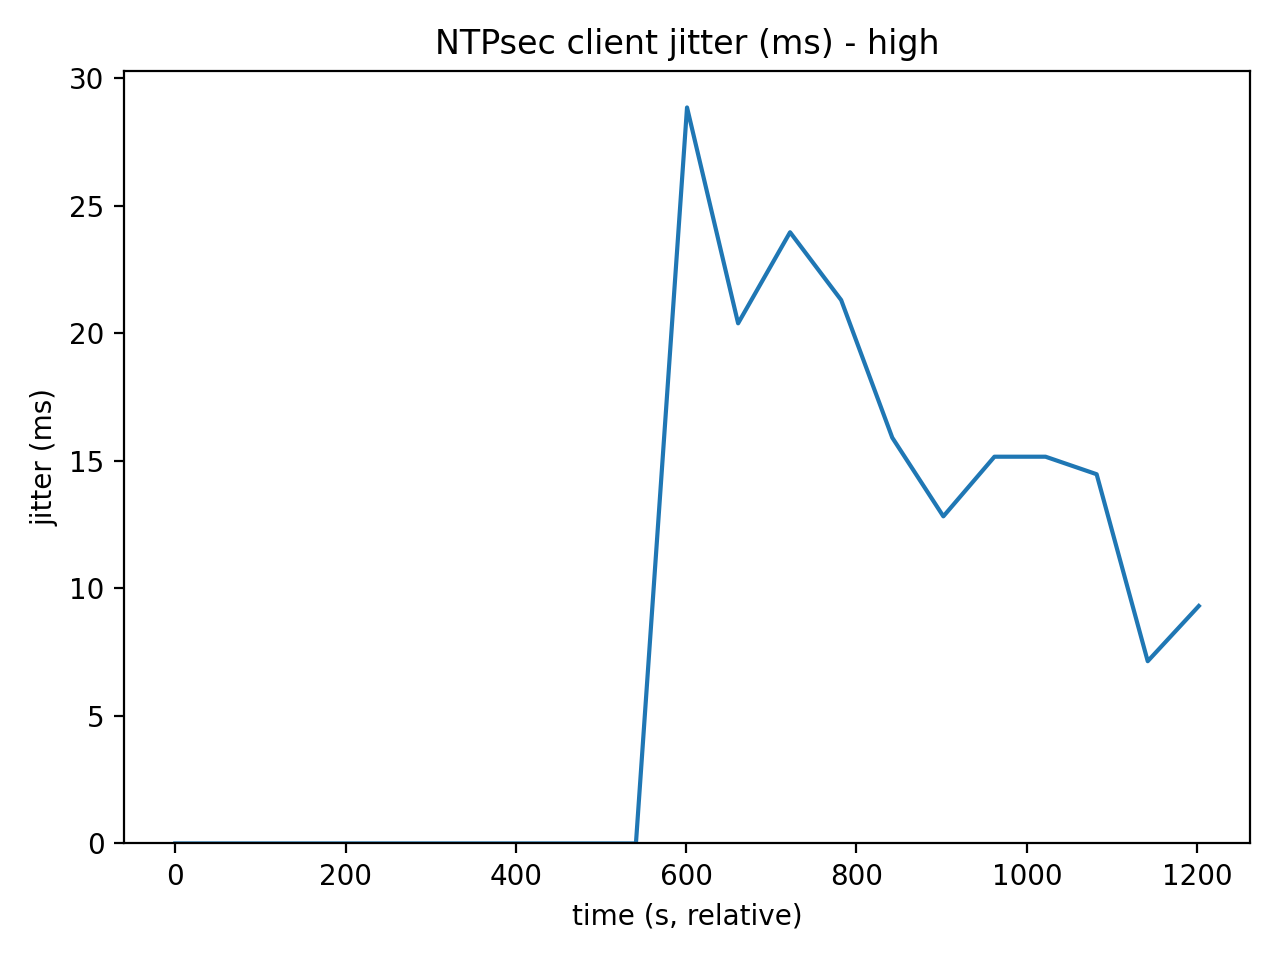
\includegraphics[width=\linewidth]{
      images/data_plots/plots_ntpsec/ntpsec_client_high_jitter_ms.png
    }
    \caption{Scenario HIGH}
  \end{subfigure}

  \caption{Comparazione della performance - nodo: \texttt{clientntp}}
  \label{fig:scenario_comparison}
\end{figure}

L’analisi del \texttt{\textbf{jitter}} rilevato sul nodo \texttt{clientntp} per
il demone \texttt{\textbf{NTPsec}} evidenzia un peggioramento progressivo della regolarità
temporale delle misurazioni al crescere della severità dello scenario di rete.
Il confronto tra i tre casi mostra infatti un incremento marcato sia del livello
della metrica sia della sua dispersione, con un passaggio netto da un regime stabile
nello scenario \texttt{low} a una condizione fortemente degradata nello scenario
\texttt{high}.

Nello scenario \texttt{low}, il jitter assume valori contenuti e si mantiene entro
una banda ristretta. Sui campioni validi si osservano una media pari a 0.5499 ms,
una mediana pari a 0.5141 ms, un primo quartile di 0.4746 ms e un terzo quartile
di 0.6281 ms, con IQR pari a 0.1535 ms. La deviazione standard è 0.0891 ms, mentre
il minimo e il massimo risultano pari rispettivamente a 0.4342 ms e 0.6951 ms.
La distribuzione appare quindi compatta e sostanzialmente regolare, senza evidenza
di valori estremi in grado di alterarne in modo significativo la struttura.

Nel caso \texttt{medium}, il jitter cresce in modo sensibile sia in termini di livello
sia in termini di dispersione. La media risulta pari a 1.7321 ms e la mediana a
1.8156 ms, con quartili pari a 1.5969 ms e 1.9073 ms e IQR di 0.3104 ms. La
deviazione standard è 0.3277 ms, il minimo è 1.1299 ms e il massimo 2.2657 ms.
Rispetto allo scenario \texttt{low}, il jitter medio risulta circa triplicato, mentre
aumentano anche l’ampiezza delle oscillazioni e la dispersione complessiva della distribuzione.

Lo scenario \texttt{high} presenta il comportamento più degradato. In questo caso
il jitter raggiunge una media pari a 16.7730 ms e una mediana pari a 15.1623 ms,
con primo quartile di 13.6496 ms, terzo quartile di 20.8481 ms e IQR pari a 7.1985
ms. La deviazione standard è 6.3757 ms, il minimo è 7.1450 ms e il massimo 28.8548
ms. Il grafico mostra una fase iniziale fortemente instabile, caratterizzata da un
picco molto elevato, seguita da una riduzione progressiva della metrica verso
valori comunque molto superiori a quelli osservati negli scenari \texttt{low} e \texttt{medium}.
La differenza tra media e mediana, insieme all’ampiezza del range, indica che la distribuzione
è influenzata da valori particolarmente elevati, pur restando nel complesso
strutturalmente collocata su livelli di forte degrado.

Nel complesso, il confronto tra i tre scenari mostra una progressione molto marcata
del jitter al crescere degli impairment di rete. La media passa da 0.5499 ms
nello scenario \texttt{low} a 1.7321 ms nel caso \texttt{medium}, fino a 16.7730 ms
nel caso \texttt{high}; analogamente, l’IQR cresce da 0.1535 ms a 0.3104 ms fino
a 7.1985 ms. Il jitter si conferma pertanto una metrica particolarmente efficace nel
mettere in evidenza l’impatto del degrado della rete sulla stabilità temporale delle
misurazioni osservate dal clientntp NTPsec.

\subsubsection{Analisi metrica: \texttt{offset}}
\begin{figure}[H]
  \centering

  \begin{subfigure}
    {0.32\textwidth}
    \centering
    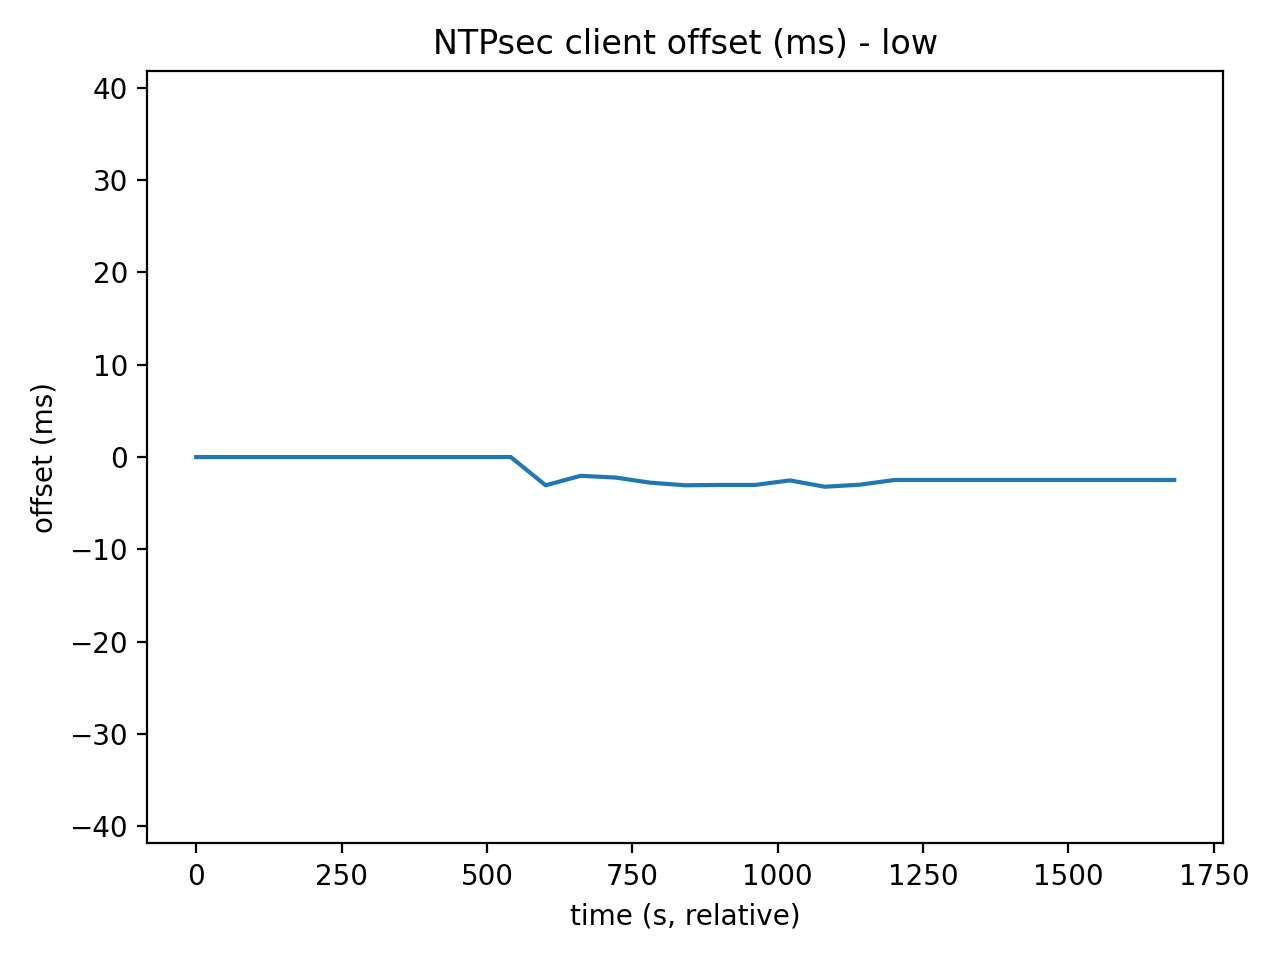
\includegraphics[width=\linewidth]{
      images/data_plots/plots_ntpsec/ntpsec_client_low_offset_ms.png
    }
    \caption{Scenario LOW}
  \end{subfigure}
  \hfill
  \begin{subfigure}
    {0.32\textwidth}
    \centering
    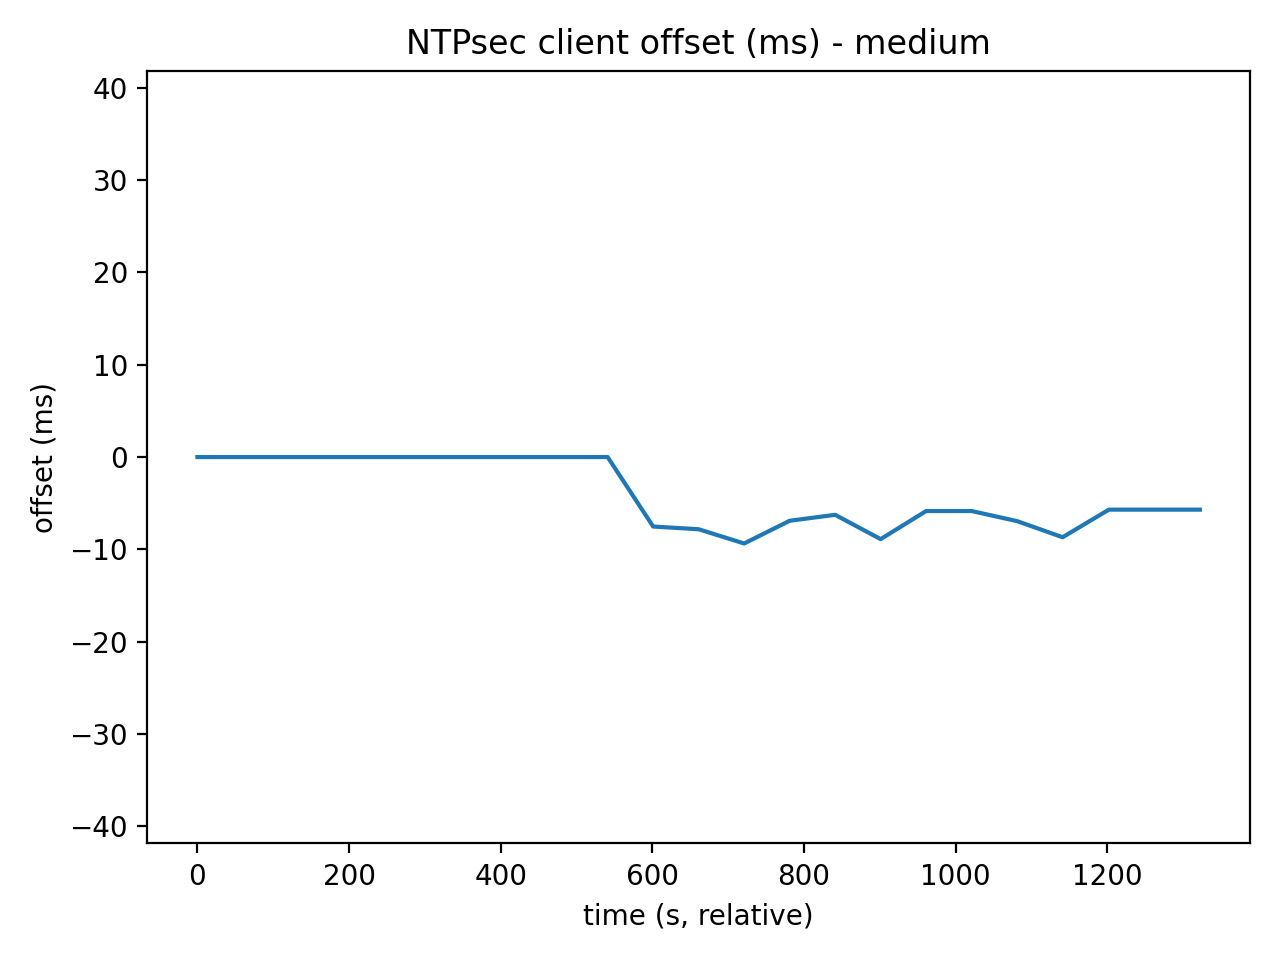
\includegraphics[width=\linewidth]{
      images/data_plots/plots_ntpsec/ntpsec_client_medium_offset_ms.png
    }
    \caption{Scenario MEDIUM}
  \end{subfigure}
  \hfill
  \begin{subfigure}
    {0.32\textwidth}
    \centering
    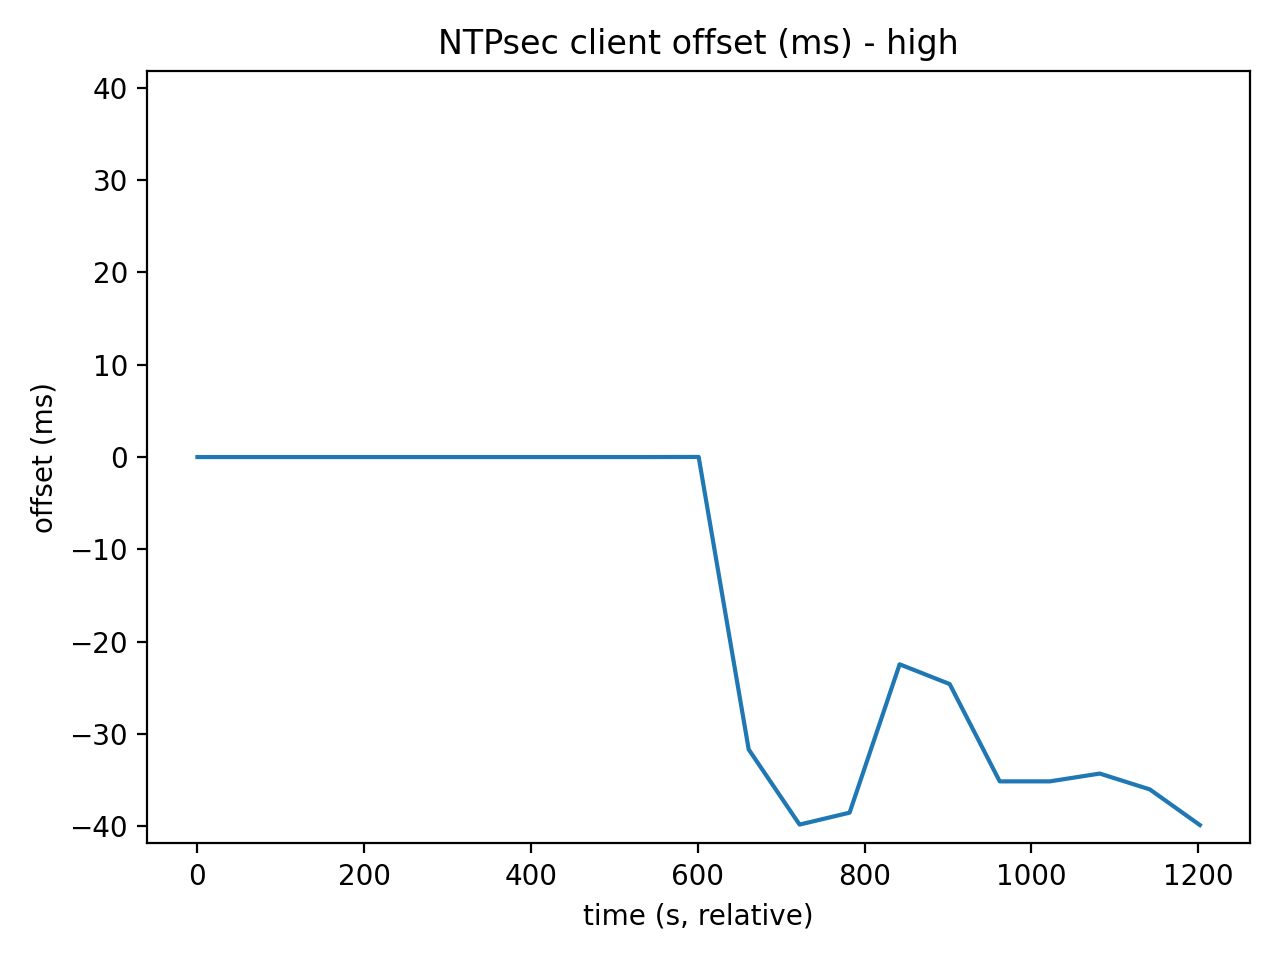
\includegraphics[width=\linewidth]{
      images/data_plots/plots_ntpsec/ntpsec_client_high_offset_ms.png
    }
    \caption{Scenario HIGH}
  \end{subfigure}

  \caption{Comparazione della performance - nodo: \texttt{clientntp}}
  \label{fig:scenario_comparison}
\end{figure}

L’analisi dell’\texttt{\textbf{offset}} misurato sul nodo \texttt{clientntp} per il
demone \texttt{\textbf{NTPsec}} evidenzia una progressiva perdita di accuratezza
della sincronizzazione al crescere della severità dello scenario di rete. Dopo la
fase iniziale di inizializzazione, in tutti e tre i casi il clientntp entra in
un regime operativo in cui l’offset assume valori sistematicamente negativi; al crescere
degli impairment, tali valori si allontanano progressivamente dallo zero e
mostrano una dispersione crescente.

Nello scenario \texttt{low}, l’offset si mantiene entro una banda relativamente
ristretta, con media pari a -2.6458 ms e mediana pari a -2.4823 ms. I quartili
sono pari a -3.0084 ms e -2.4823 ms, con IQR di 0.5261 ms. Il minimo e il
massimo risultano rispettivamente pari a -3.2148 ms e -2.0321 ms, mentre la deviazione
standard è 0.3248 ms. Il grafico mostra un andamento regolare e stabile, collocato
attorno a valori moderatamente negativi, indicativo di una sincronizzazione
ancora relativamente accurata.

Nel caso \texttt{medium}, l’offset si sposta in modo netto verso valori più
negativi. La media risulta pari a -7.0136 ms e la mediana a -6.9026 ms, con
quartili pari a -7.8200 ms e -5.8483 ms e IQR di 1.9717 ms. Il minimo è -9.3643
ms, il massimo -5.6966 ms e la deviazione standard 1.3313 ms. Rispetto allo scenario
\texttt{low}, il valore tipico dell’offset si allontana quindi in modo sensibile dallo
zero, mentre cresce anche la dispersione complessiva della metrica.

Lo scenario \texttt{high} presenta il comportamento più degradato. In questo
caso l’offset assume media pari a -30.6788 ms e mediana pari a -35.1341 ms, con quartili
di -37.2646 ms e -28.1322 ms e IQR di 9.1325 ms. Il minimo osservato è -39.8648 ms,
mentre il massimo è 0.0131 ms. Il grafico mostra che, dopo un primo campione
prossimo allo zero, la serie entra rapidamente in un regime fortemente negativo,
senza più tornare verso i livelli osservati negli scenari precedenti. La differenza
tra media e mediana indica che la distribuzione è influenzata da tale campione iniziale,
mentre la mediana descrive più fedelmente il livello tipico dell’offset in
regime, pari a circa -35 ms.

Nel complesso, il confronto tra i tre scenari mostra una progressione molto marcata
dell’offset in valore assoluto: la media passa da -2.6458 ms nello scenario \texttt{low}
a -7.0136 ms nel caso \texttt{medium}, fino a -30.6788 ms nel caso \texttt{high};
analogamente, l’IQR cresce da 0.5261 ms a 1.9717 ms fino a 9.1325 ms. L’offset
si conferma pertanto una metrica particolarmente efficace nel mettere in
evidenza l’impatto del degrado della rete sull’accuratezza e sulla stabilità del
processo di sincronizzazione del clientntp NTPsec.

\subsection{\texttt{boundary}}
Nel caso del nodo \texttt{boundary}, l’interpretazione dei risultati richiede
una precisazione preliminare. A differenza di quanto osservato sul nodo \texttt{clientntp},
gli impairment di rete introdotti mediante \texttt{tc/netem} non agiscono
direttamente sul collegamento \texttt{upstream} tra il nodo \texttt{boundary} e
il nodo di riferimento, bensì sul ramo \texttt{downstream} tra \texttt{boundary} e
\texttt{clientntp}. Ne consegue che le metriche rilevate sul \texttt{boundary}
non dovrebbero, in linea teorica, risentire in modo marcato del degrado
introdotto nei tre scenari sperimentali, o comunque non con la stessa intensità osservata
nel caso del clientntp.

L’analisi delle metriche del nodo \texttt{boundary} è pertanto orientata
principalmente a verificare la coerenza tra tale aspettativa teorica e i dati
effettivamente osservati. In particolare, il confronto tra scenari è finalizzato
a stabilire se le eventuali differenze rilevate siano effettivamente contenute, come
atteso, oppure se emergano variazioni non trascurabili che possano suggerire
effetti indiretti del degrado di rete sul comportamento del nodo.

Va inoltre considerato che il tempo di ingresso nel regime operativo può
differire rispetto a quello osservato sul nodo \texttt{clientntp}. Tale aspetto
viene tenuto in considerazione nell’interpretazione dei risultati, pur non costituendo,
di per sé, l’oggetto principale del confronto tra scenari.

\subsubsection{Analisi metriche: \texttt{delay, jitter, offset}}
\begin{figure}[H]
  \centering

  \begin{subfigure}
    {0.32\textwidth}
    \centering
    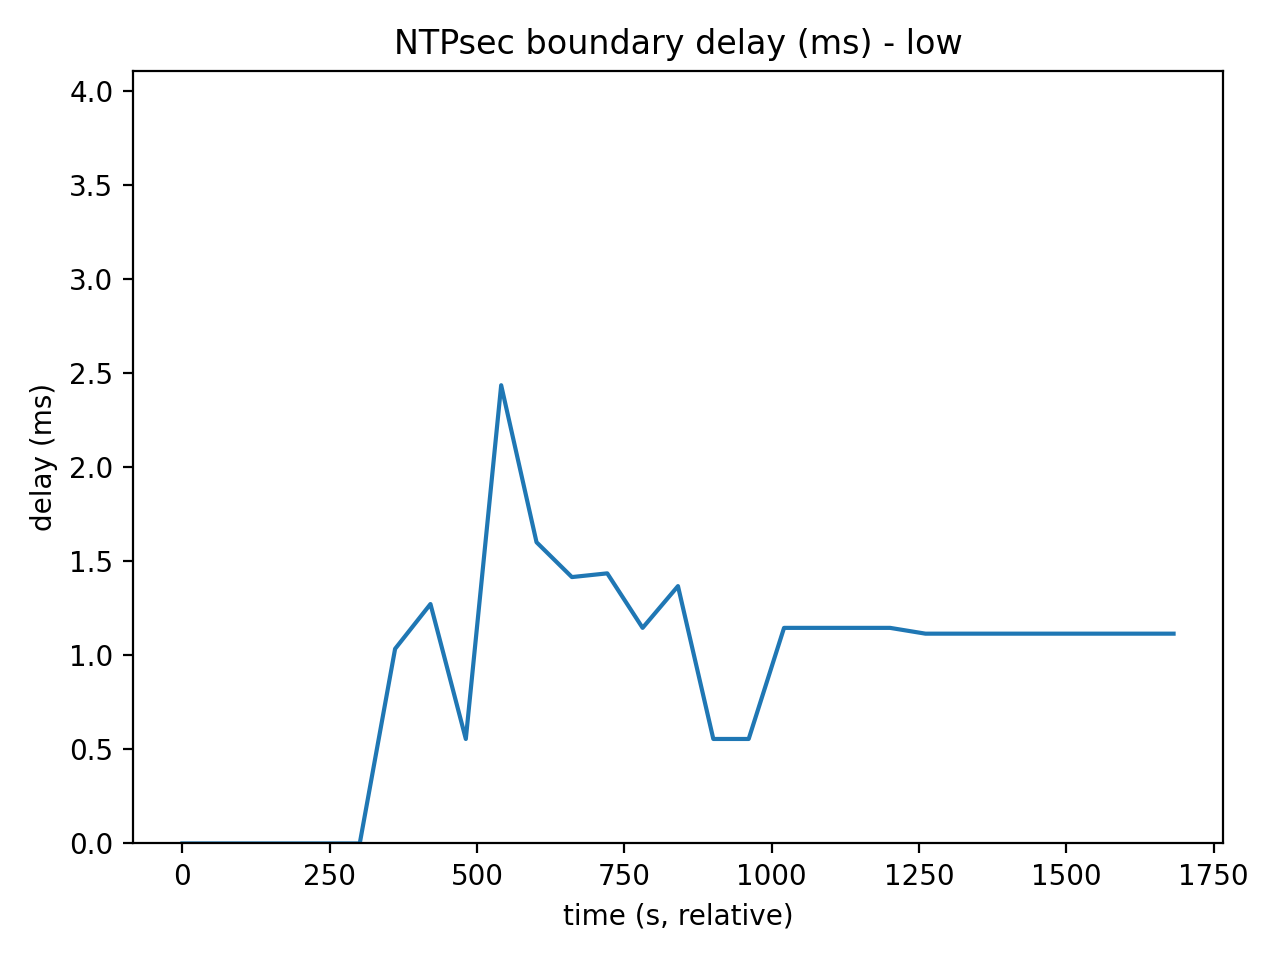
\includegraphics[width=\linewidth]{
      images/data_plots/plots_ntpsec/ntpsec_boundary_low_delay_ms.png
    }
    \caption{Scenario LOW}
  \end{subfigure}
  \hfill
  \begin{subfigure}
    {0.32\textwidth}
    \centering
    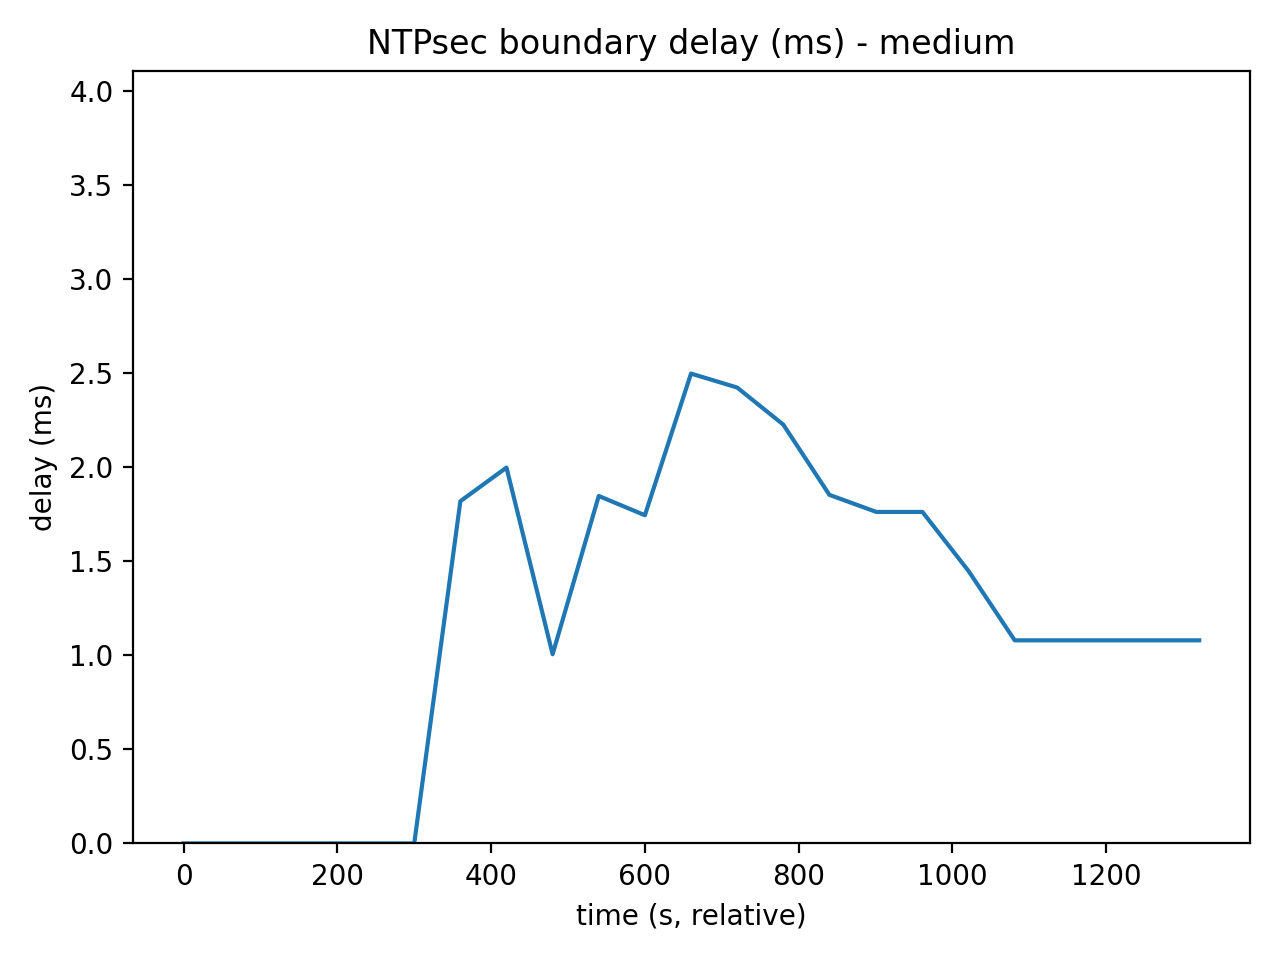
\includegraphics[width=\linewidth]{
      images/data_plots/plots_ntpsec/ntpsec_boundary_medium_delay_ms.png
    }
    \caption{Scenario MEDIUM}
  \end{subfigure}
  \hfill
  \begin{subfigure}
    {0.32\textwidth}
    \centering
    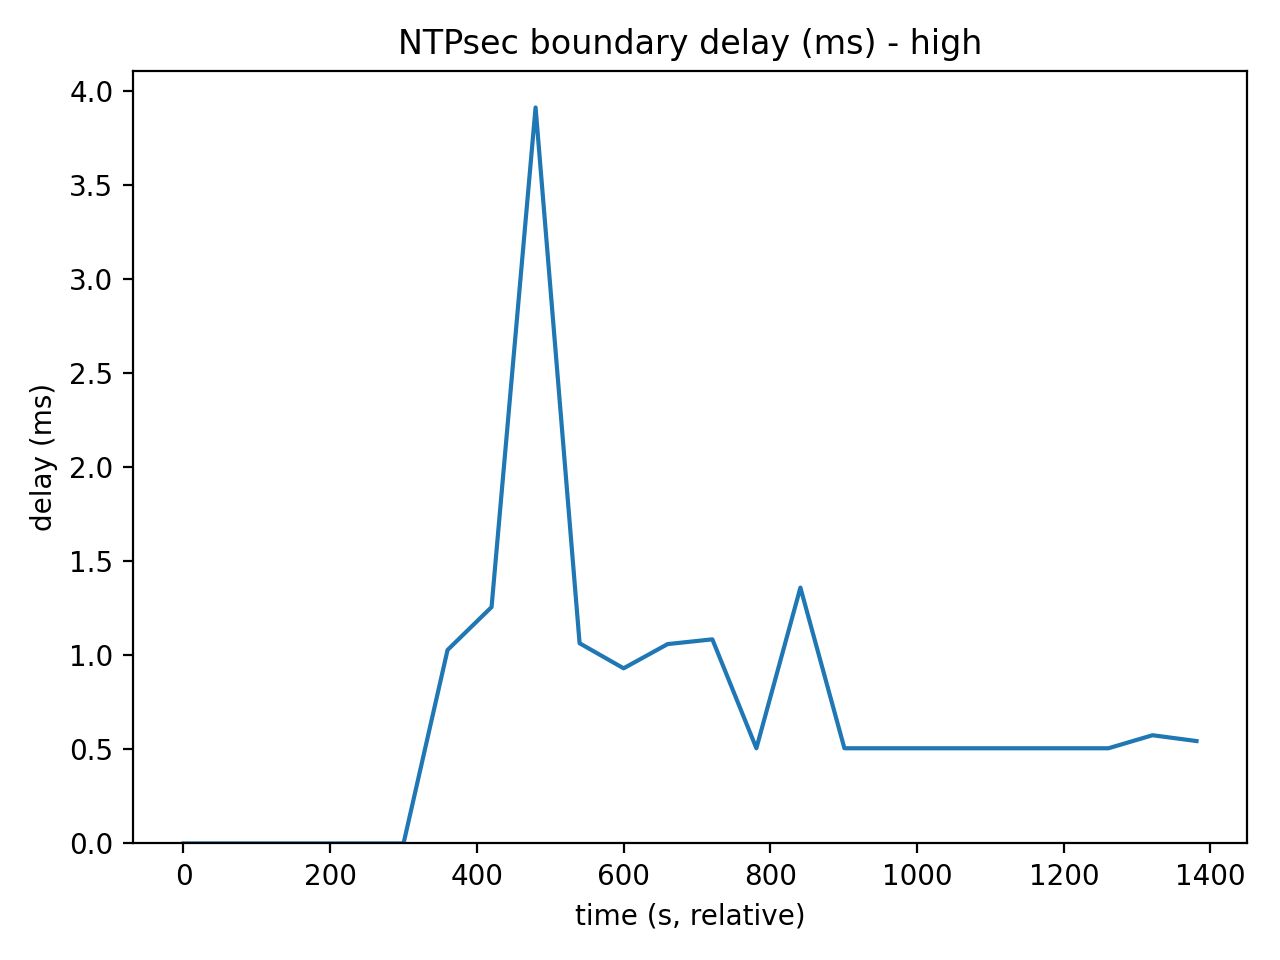
\includegraphics[width=\linewidth]{
      images/data_plots/plots_ntpsec/ntpsec_boundary_high_delay_ms.png
    }
    \caption{Scenario HIGH}
  \end{subfigure}

  \caption{Comparazione della performance - nodo: \texttt{boundary} metrica: \texttt{delay}}
  \label{fig:scenario_comparison}
\end{figure}

\begin{figure}[H]
  \centering

  \begin{subfigure}
    {0.32\textwidth}
    \centering
    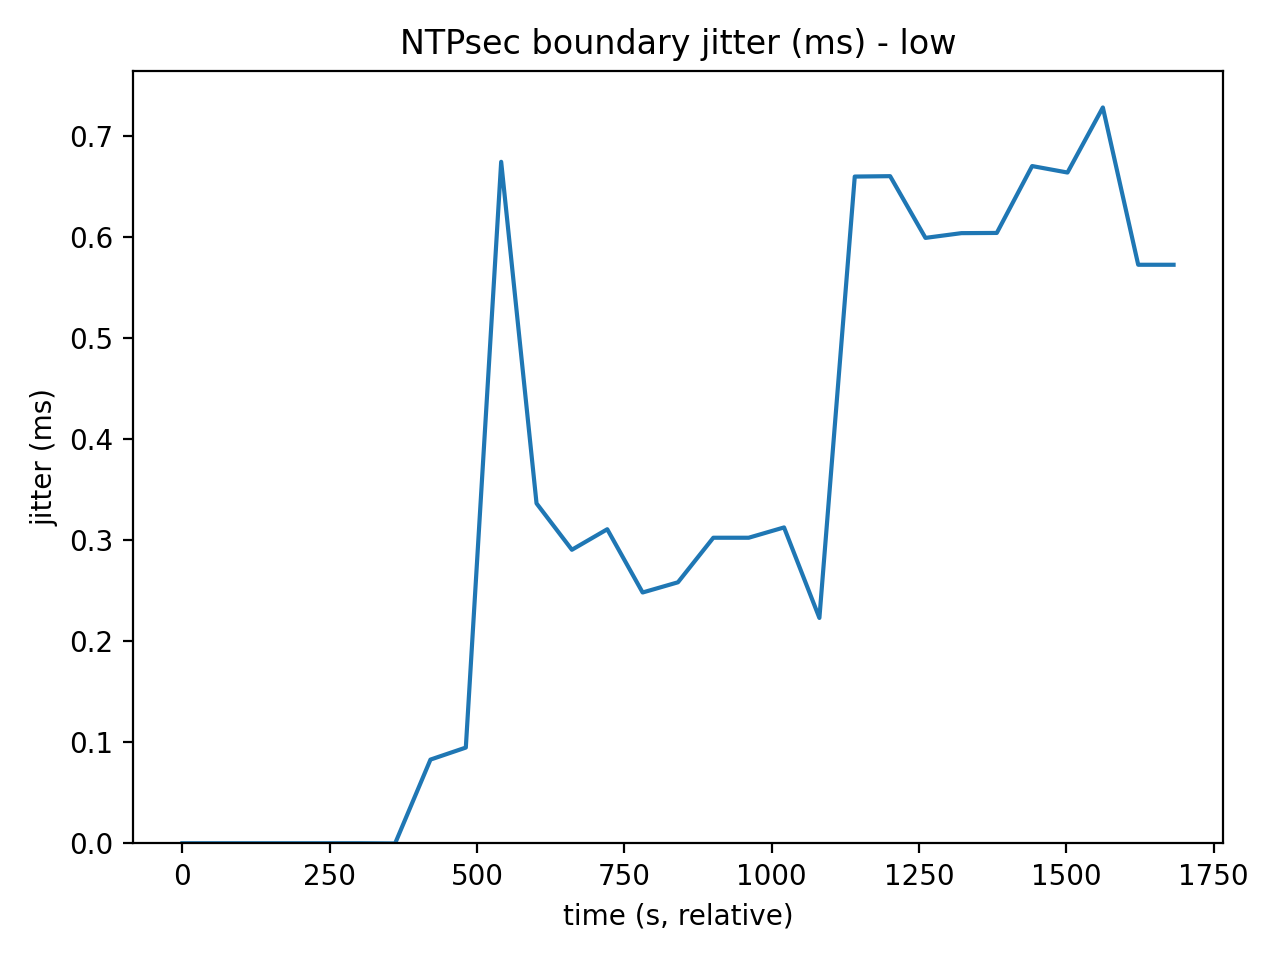
\includegraphics[width=\linewidth]{
      images/data_plots/plots_ntpsec/ntpsec_boundary_low_jitter_ms.png
    }
    \caption{Scenario LOW}
  \end{subfigure}
  \hfill
  \begin{subfigure}
    {0.32\textwidth}
    \centering
    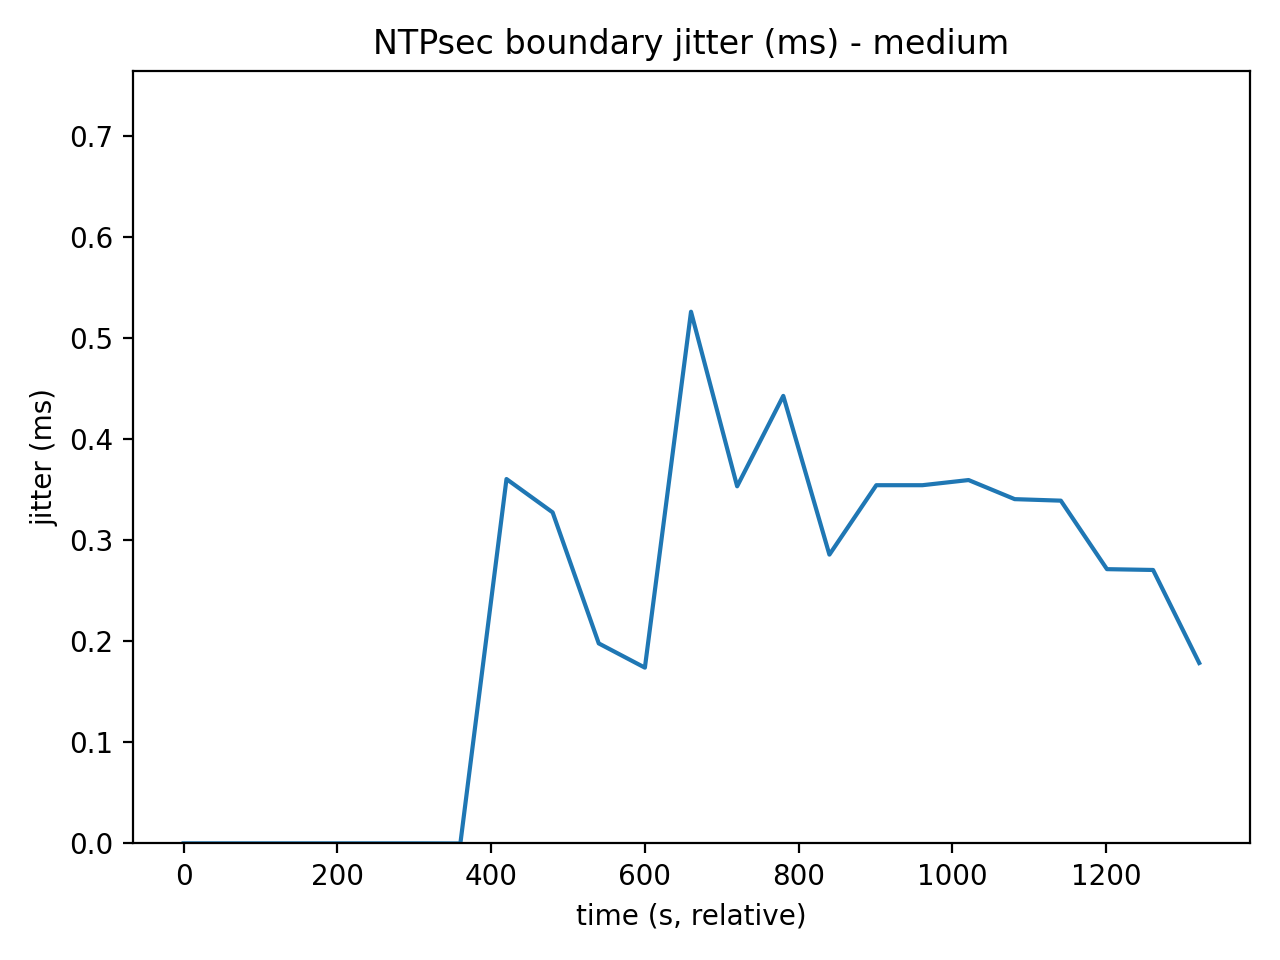
\includegraphics[width=\linewidth]{
      images/data_plots/plots_ntpsec/ntpsec_boundary_medium_jitter_ms.png
    }
    \caption{Scenario MEDIUM}
  \end{subfigure}
  \hfill
  \begin{subfigure}
    {0.32\textwidth}
    \centering
    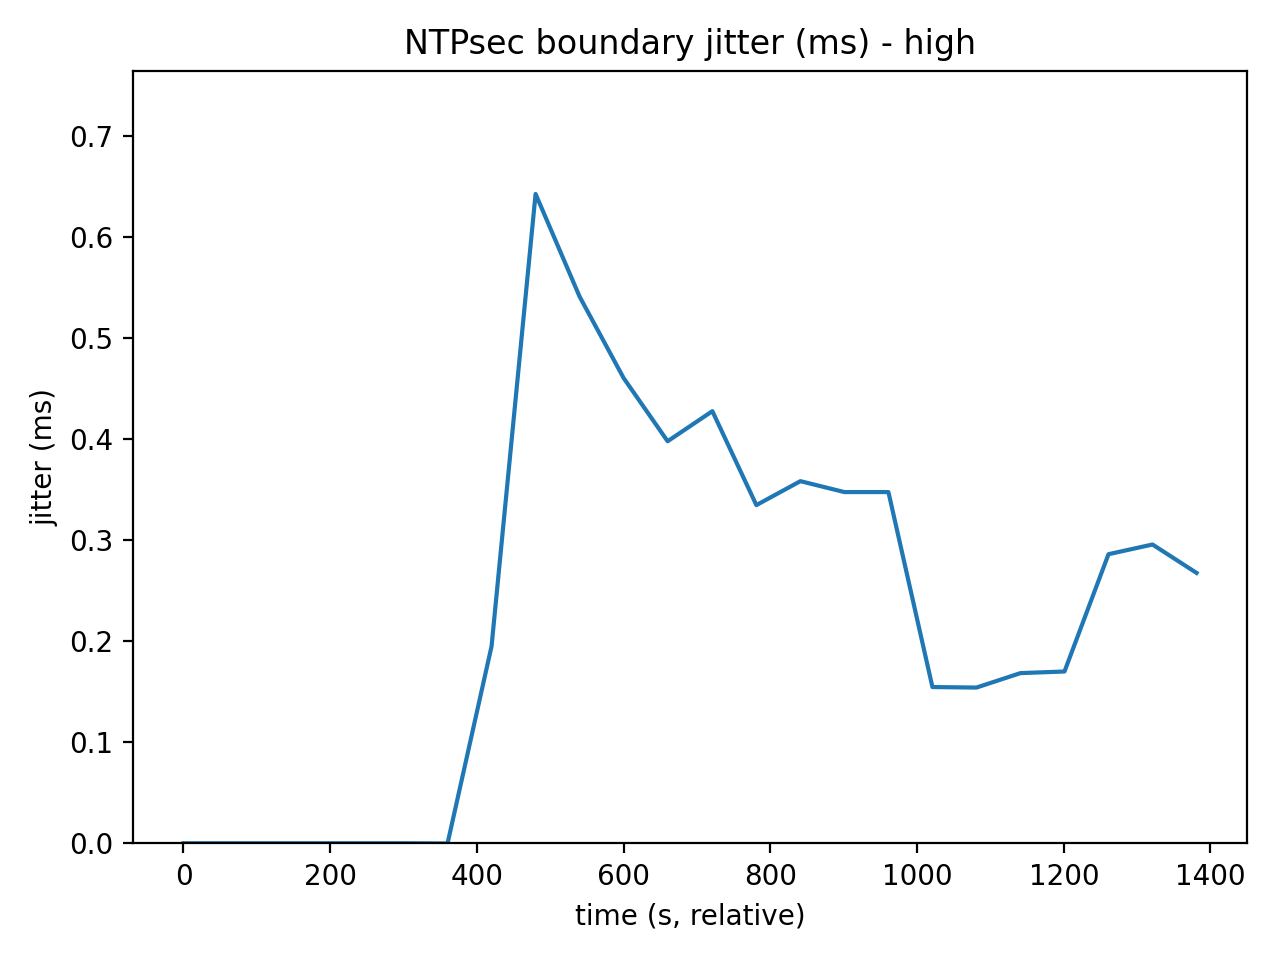
\includegraphics[width=\linewidth]{
      images/data_plots/plots_ntpsec/ntpsec_boundary_high_jitter_ms.png
    }
    \caption{Scenario HIGH}
  \end{subfigure}

  \caption{Comparazione della performance - nodo: \texttt{boundary} metrica: \texttt{jitter}}
  \label{fig:scenario_comparison}
\end{figure}

\begin{figure}[H]
  \centering

  \begin{subfigure}
    {0.32\textwidth}
    \centering
    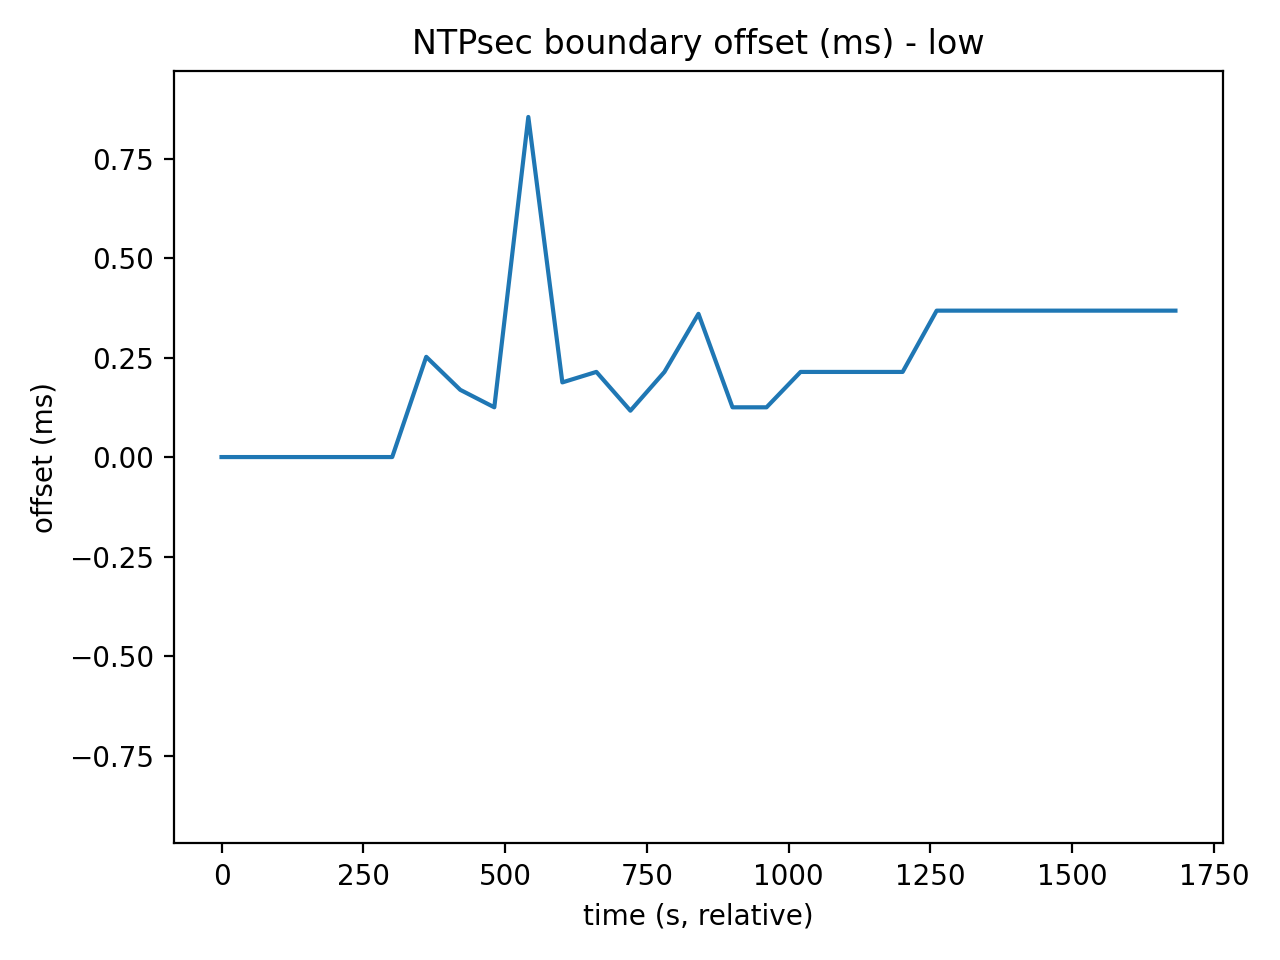
\includegraphics[width=\linewidth]{
      images/data_plots/plots_ntpsec/ntpsec_boundary_low_offset_ms.png
    }
    \caption{Scenario LOW}
  \end{subfigure}
  \hfill
  \begin{subfigure}
    {0.32\textwidth}
    \centering
    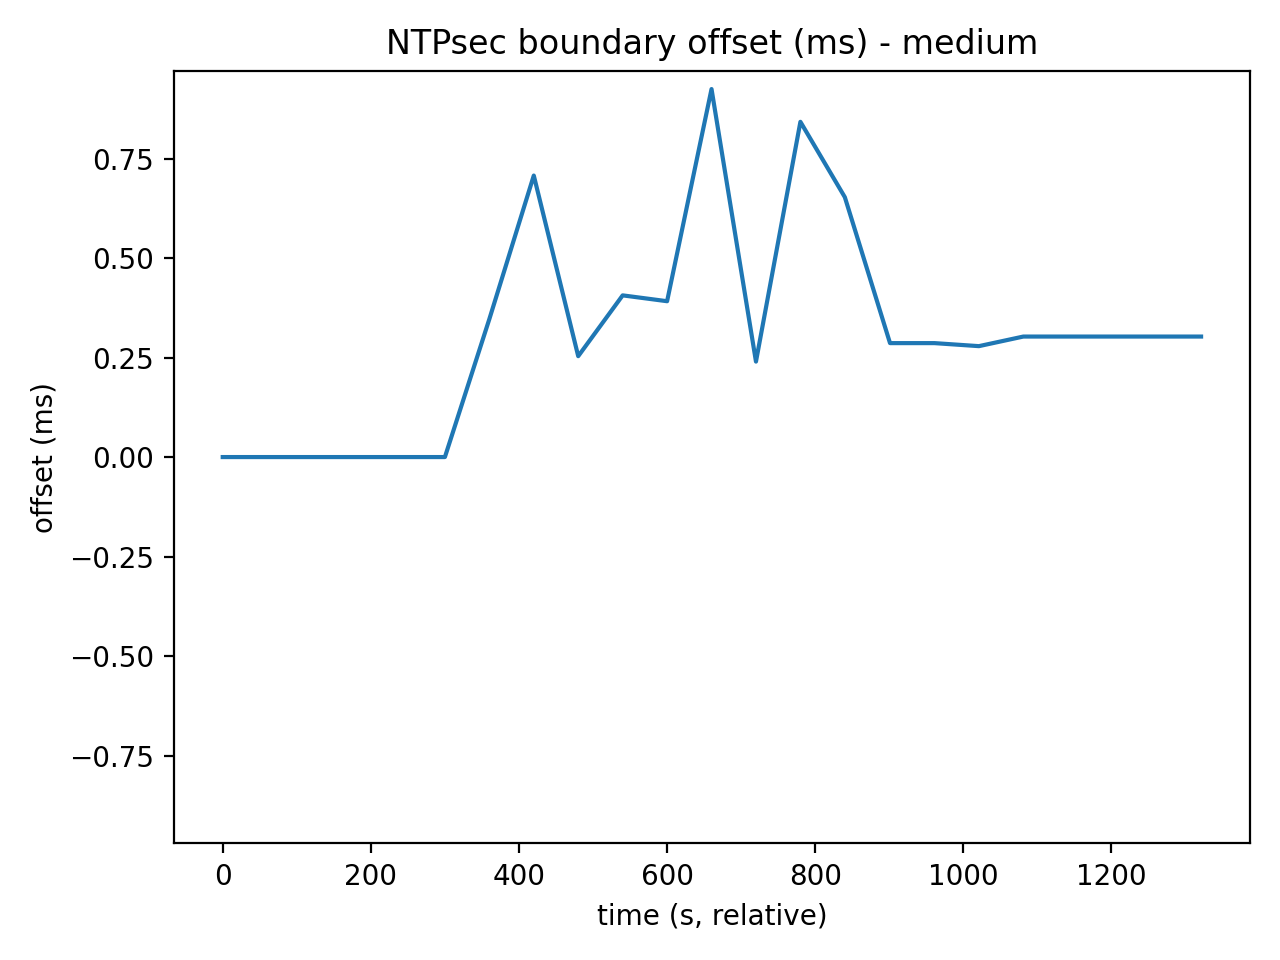
\includegraphics[width=\linewidth]{
      images/data_plots/plots_ntpsec/ntpsec_boundary_medium_offset_ms.png
    }
    \caption{Scenario MEDIUM}
  \end{subfigure}
  \hfill
  \begin{subfigure}
    {0.32\textwidth}
    \centering
    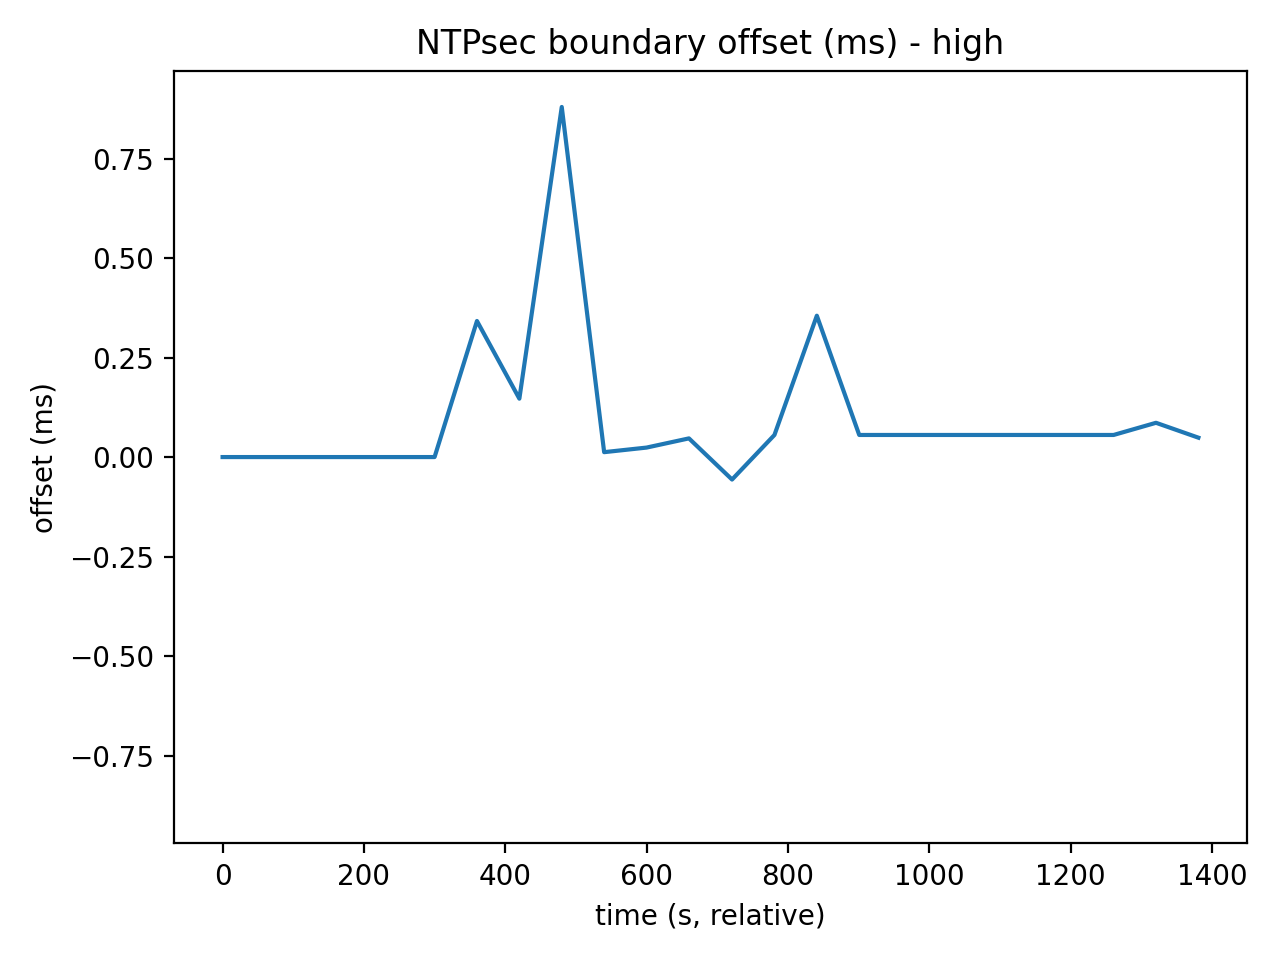
\includegraphics[width=\linewidth]{
      images/data_plots/plots_ntpsec/ntpsec_boundary_high_offset_ms.png
    }
    \caption{Scenario HIGH}
  \end{subfigure}

  \caption{Comparazione della performance - nodo: \texttt{boundary} metrica: \texttt{offset}}
  \label{fig:scenario_comparison}
\end{figure}

Nel caso del nodo \texttt{boundary}, il confronto tra scenari non evidenzia un
degrado sistematico e paragonabile a quello osservato precedentemente nel
\texttt{clientntp}. Tale risultato è coerente con la configurazione sperimentale
adottata: gli impairment di rete introdotti mediante \texttt{tc/netem} agiscono
infatti sul ramo \texttt{downstream} tra \texttt{boundary} e \texttt{clientntp},
mentre le metriche qui considerate descrivono il comportamento del nodo \texttt{boundary}
rispetto al proprio riferimento \texttt{upstream} con il nodo \texttt{servergm},
non direttamente soggetto al degrado configurato.

Un primo elemento coerente con tale interpretazione riguarda il tempo di
ingresso nel regime operativo. Nei tre scenari, il nodo \texttt{boundary} raggiunge
infatti i primi campioni validi attorno a $540$–$541$ secondi, quindi in
anticipo rispetto al nodo \texttt{clientntp}, per il quale i campioni validi
iniziano a circa $601$ secondi. Ciò suggerisce che il processo di selezione e stabilizzazione
della sorgente risulta meno penalizzato sul ramo \texttt{upstream} osservato dal
\texttt{boundary}.

Anche l’analisi delle singole metriche conferma l’assenza di un degrado netto al crescere
della severità dello scenario. Il \texttt{delay} medio passa da 1.2016 ms nello scenario
\texttt{low} a 1.6412 ms nel caso \texttt{medium}, per poi ridursi a 0.7116 ms
nello scenario \texttt{high}. L’\texttt{offset} medio rimane in tutti i casi
contenuto e prossimo allo zero, con valori pari a 0.2998 ms, 0.4159 ms e 0.0640
ms rispettivamente nei tre scenari. Analogamente, il \texttt{jitter} resta su livelli
bassi e relativamente stabili, assumendo valori medi pari a 0.4799 ms nel caso
\texttt{low}, 0.3179 ms nel caso \texttt{medium} e 0.3143 ms nel caso \texttt{high}.

Nel complesso, le differenze osservate tra scenari risultano moderate e non seguono
una progressione monotona con l’aumentare degli impairment. Questo comportamento
suggerisce che il nodo \texttt{boundary} mantiene una condizione di sincronizzazione
sostanzialmente stabile rispetto al proprio collegamento di riferimento, e che
l’effetto del degrado introdotto sulla rete si manifesta in modo molto marcato
solamente sul nodo \texttt{clientntp} che non sul \texttt{boundary}. Le variazioni
residue osservate nelle metriche del \texttt{boundary} possono pertanto essere
interpretate come oscillazioni contenute del processo di sincronizzazione, piuttosto
che come evidenza di un deterioramento strutturale legato allo scenario sperimentale.

\section{\texttt{ptp4l}}
L’analisi dei dati relativa al demone \texttt{\textbf{ptp4l}} è articolata in
funzione dei nodi della topologia sui quali sono state rilevate le metriche di
interesse. In particolare, l’attenzione è rivolta ai nodi \texttt{clientptp} e \texttt{boundary},
per i quali sono disponibili misurazioni direttamente riconducibili al comportamento
del protocollo in termini di sincronizzazione e ritardo.

Il nodo \texttt{servergm}, al contrario, non fornisce una serie di metriche
comparabili a quelle osservate sugli altri nodi, poiché il relativo output è limitato
essenzialmente allo stato di inizializzazione del demone e alla selezione del clock
locale come \texttt{best master}. Per tale ragione, esso non viene incluso
nell’analisi quantitativa presentata in questa sezione.

Anche nel caso di \texttt{\textbf{ptp4l}}, gli impairment di rete introdotti
mediante \texttt{tc/netem} sono applicati sul ramo \texttt{downstream} a valle
del nodo \texttt{boundary}. Ne consegue che il confronto tra scenari assume un
significato diverso a seconda del nodo osservato: nel caso del \texttt{clientptp},
le metriche possono riflettere in modo diretto il degrado introdotto sulla rete,
mentre nel caso del \texttt{boundary} ci si attende, in linea teorica, un impatto
più contenuto, poiché il collegamento verso il nodo di riferimento non è quello
direttamente soggetto agli impairment configurati.

Alla luce di ciò, l’analisi viene sviluppata separatamente per i nodi \texttt{clientptp}
e \texttt{boundary}, così da evidenziare sia gli effetti diretti del degrado di
rete sul nodo terminale, sia l’eventuale presenza di variazioni indirette sul nodo
intermedio della topologia.

\subsection{\texttt{clientptp}}
Nel caso del nodo \texttt{clientptp}, l’analisi quantitativa delle metriche non può
essere estesa in modo uniforme a tutti e tre gli scenari sperimentali. In
particolare, nello scenario \texttt{high} non viene raggiunta una condizione
operativa stabile tale da produrre una serie di campioni utilizzabile per il
calcolo delle metriche considerate. Per tale ragione, i confronti quantitativi
sul nodo \texttt{clientptp} sono necessariamente limitati ai soli scenari \texttt{low}
e \texttt{medium}.

Nello scenario \texttt{high} non si raggiunge una condizione di sincronizzazione
stabile: il log mostra ripetute selezioni del clock locale come miglior master e un
solo tentativo transitorio di passaggio verso un master esterno, seguito
tuttavia da ritorno allo stato di \texttt{LISTENING}. L’assenza di campioni
numerici confrontabili nello scenario \texttt{high} rappresenta dunque un risultato
sperimentale, e segnala un livello di degrado tale da impedire la normale
operatività del client PTP. Il relativo output grezzo viene comunque richiamato a
supporto di tale evidenza qualitativa.

\subsubsection{Analisi metrica: \texttt{path Delay}}
\begin{figure}[H]
  \centering

  \begin{subfigure}
    {0.4\textwidth}
    \centering
    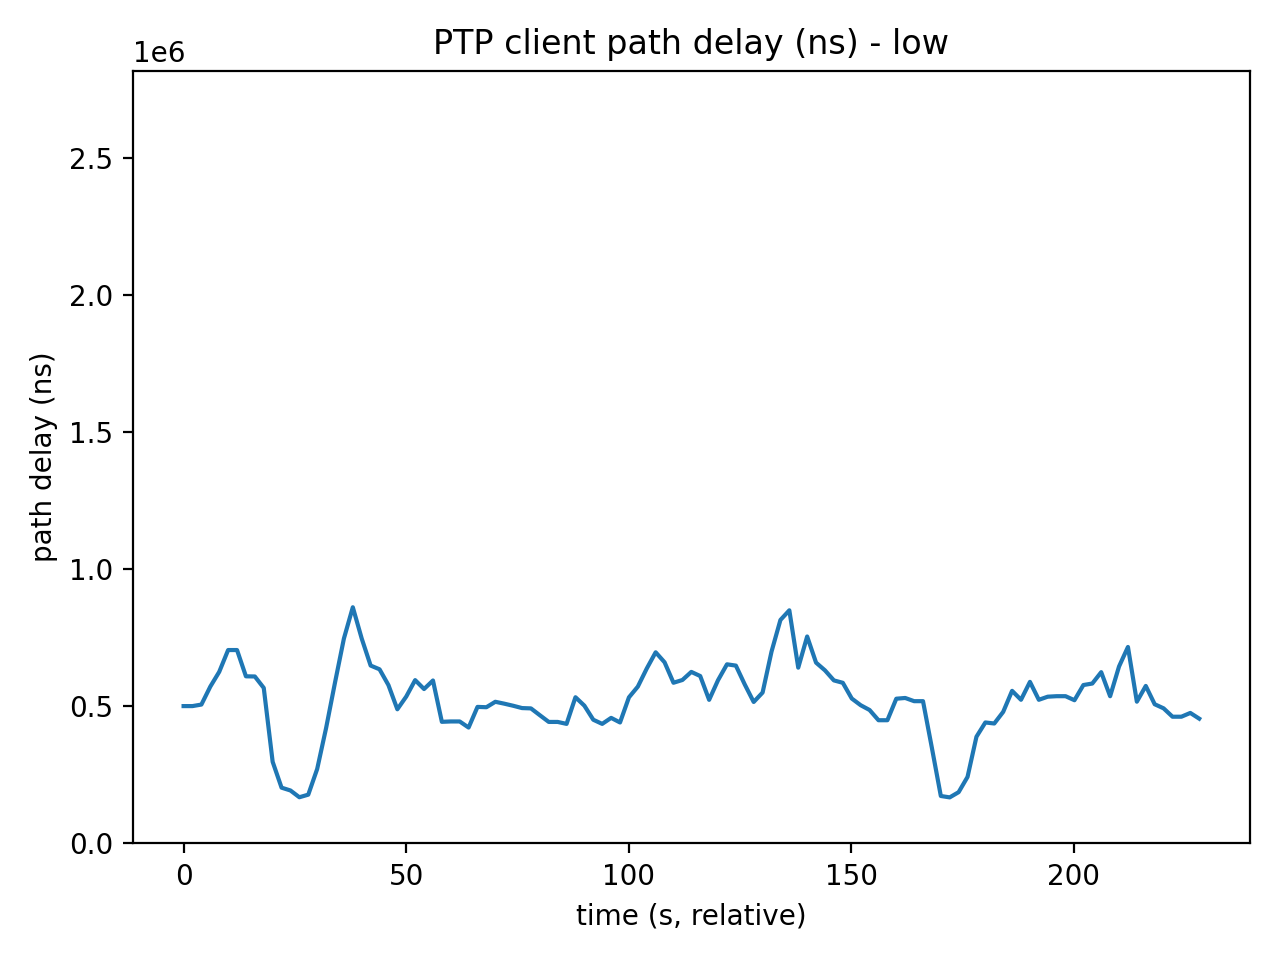
\includegraphics[width=\linewidth]{
      images/data_plots/plots_ptp/client_low_path_delay_ns.png
    }
    \caption{Scenario LOW}
  \end{subfigure}
  \hfill
  \begin{subfigure}
    {0.4\textwidth}
    \centering
    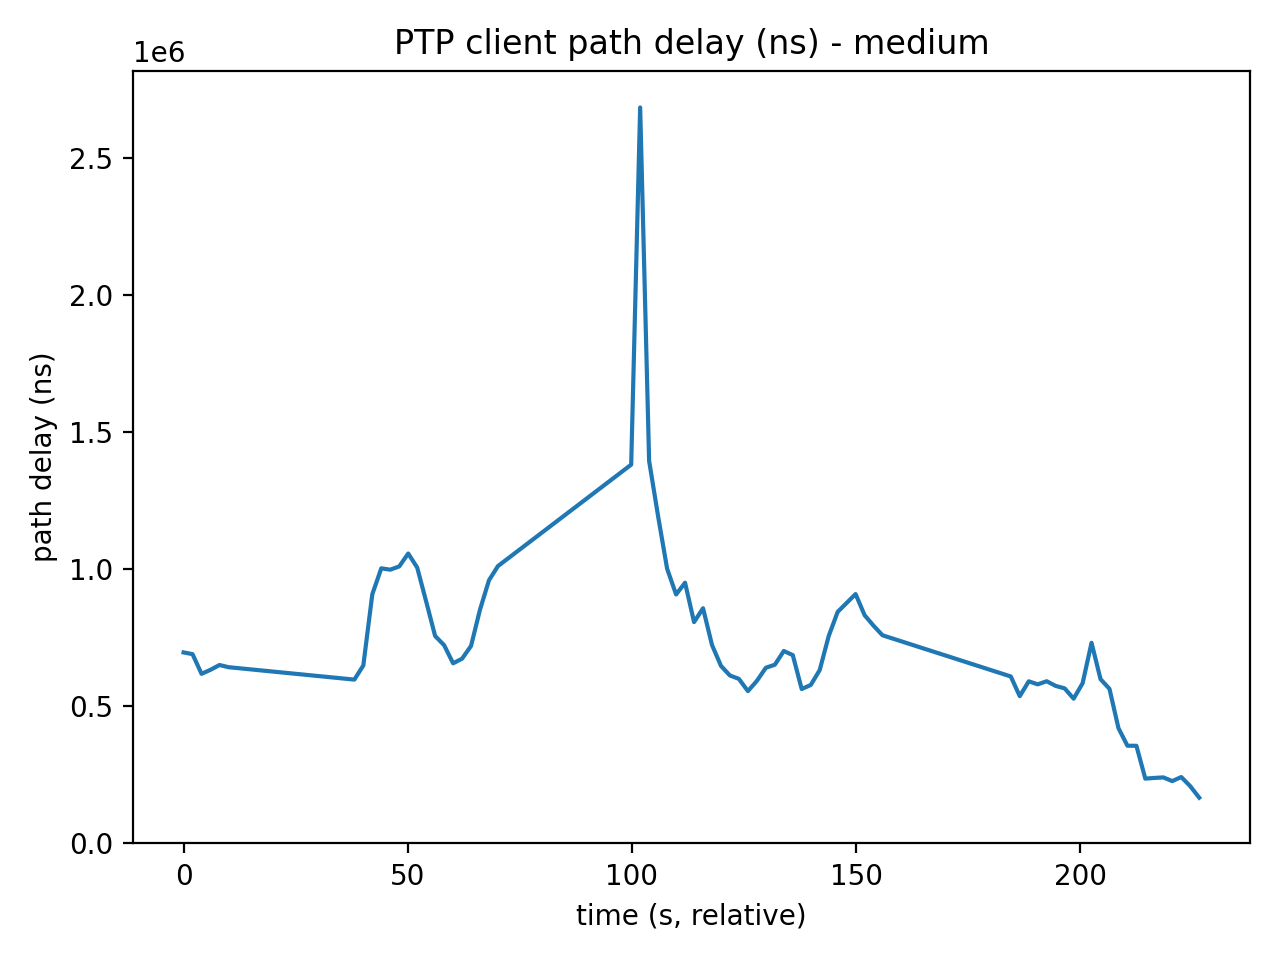
\includegraphics[width=\linewidth]{
      images/data_plots/plots_ptp/client_medium_path_delay_ns.png
    }
    \caption{Scenario MEDIUM}
  \end{subfigure}
  \caption{Comparazione della performance - nodo: \texttt{clientptp}}
  \label{fig:scenario_comparison}
\end{figure}

Nei due scenari per cui sono disponibili misurazioni, il comportamento del \texttt{path
delay} evidenzia una differenza netta tra \texttt{low} e \texttt{medium}. Nel caso
\texttt{low}, il segnale si mantiene per gran parte del tempo in una banda relativamente
contenuta, centrata attorno a valori prossimi a mezzo millisecondo. Il grafico mostra
oscillazioni presenti ma non strutturalmente divergenti, con alcuni picchi
locali e alcune discese temporanee, che tuttavia non alterano il quadro complessivo
di moderata variabilità. Le statistiche confermano tale andamento: la media è pari
a 524322.76 ns, la mediana a 524299 ns e la deviazione standard a 135730.23 ns, con
coefficiente di variazione pari a 0.259. Anche la distanza interquartile, pari a 135604
ns, risulta coerente con una dispersione contenuta. In altri termini, nello
scenario \texttt{low} il client stima un ritardo di percorso abbastanza stabile,
pur in presenza di normali fluttuazioni campionarie.

Nel caso \texttt{medium}, il comportamento cambia in modo evidente. Il livello centrale
della serie si sposta verso l’alto, con media pari a 720708.99 ns e mediana pari
a 654933 ns, quindi con un incremento sensibile rispetto allo scenario \texttt{low}.
Anche la dispersione cresce in maniera marcata: la deviazione standard sale a
340459.97 ns e il coefficiente di variazione raggiunge 0.472, quasi il doppio del
caso \texttt{low}. Il grafico mostra infatti una dinamica più irregolare,
caratterizzata da escursioni ampie, da una fase centrale con valori elevati e da un
picco massimo di 2686221 ns, molto superiore a quello osservato nello scenario
\texttt{low} (862114 ns). Anche l’intervallo interquartile aumenta fino a
275275.25 ns, confermando che l’incremento di variabilità non è dovuto solo a pochi
valori estremi, ma riguarda più in generale l’intera distribuzione delle misure.

Il confronto tra i due scenari mostra quindi che, sul nodo \texttt{clientptp}, il
passaggio da \texttt{low} a \texttt{medium} determina sia un aumento del ritardo stimato
lungo il percorso sia una riduzione della sua stabilità. Il risultato è coerente
con un peggioramento della qualità del cammino di rete osservato dal client: il \texttt{path
delay} non soltanto cresce in valore medio, ma diventa anche meno prevedibile e più
soggetto a variazioni impulsive. In questo senso, la metrica risulta sensibile al
degrado delle condizioni sperimentali già nel passaggio intermedio, mentre nello
scenario \texttt{high} il deterioramento è tale da impedire del tutto la costruzione
di una serie metrica analizzabile.

\subsubsection{Analisi metrica: \texttt{RMS offset}}
\begin{figure}[H]
  \centering

  \begin{subfigure}
    {0.4\textwidth}
    \centering
    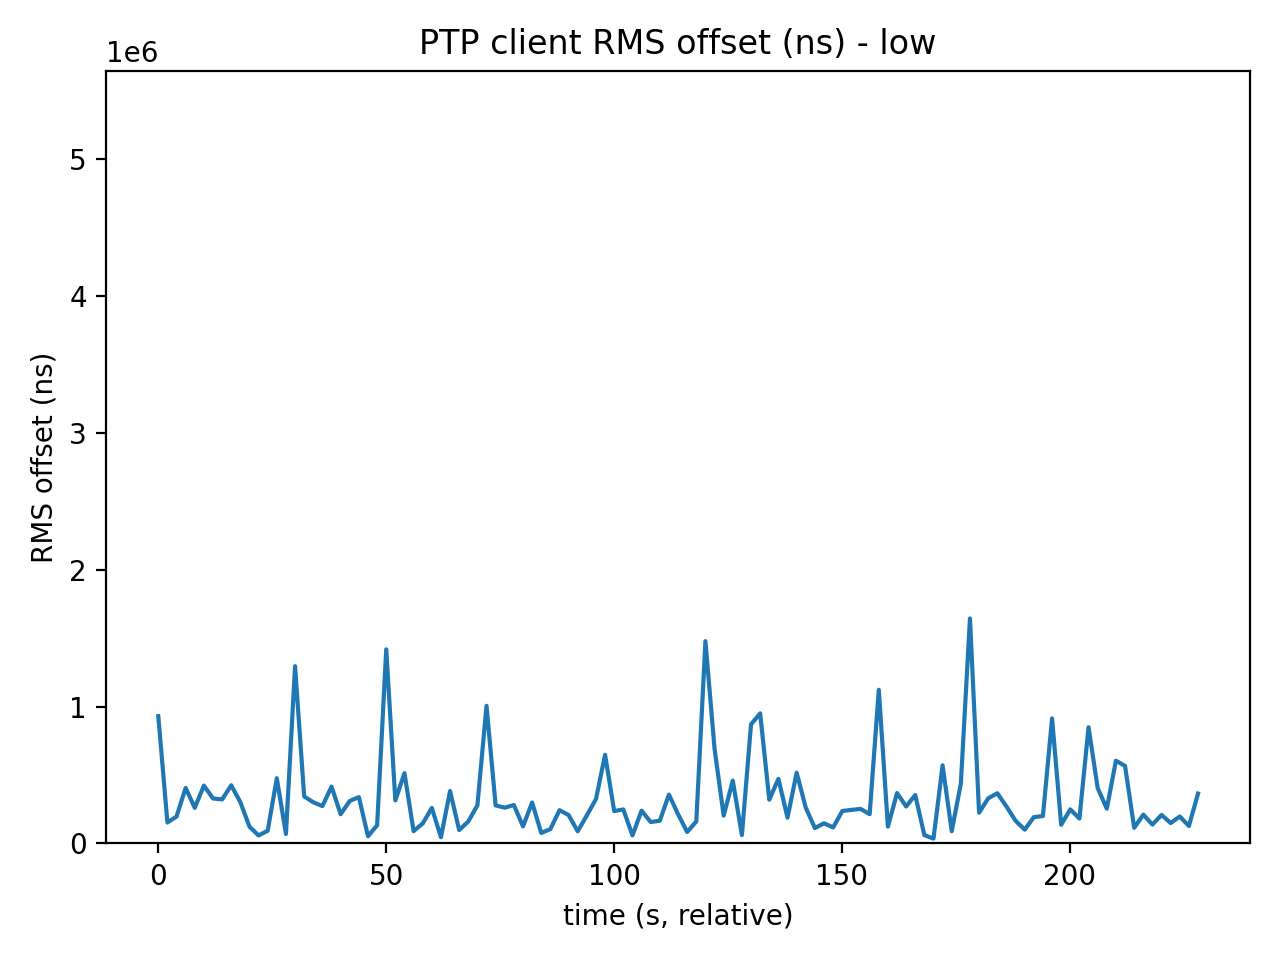
\includegraphics[width=\linewidth]{
      images/data_plots/plots_ptp/client_low_rms_ns.png
    }
    \caption{Scenario LOW}
  \end{subfigure}
  \hfill
  \begin{subfigure}
    {0.4\textwidth}
    \centering
    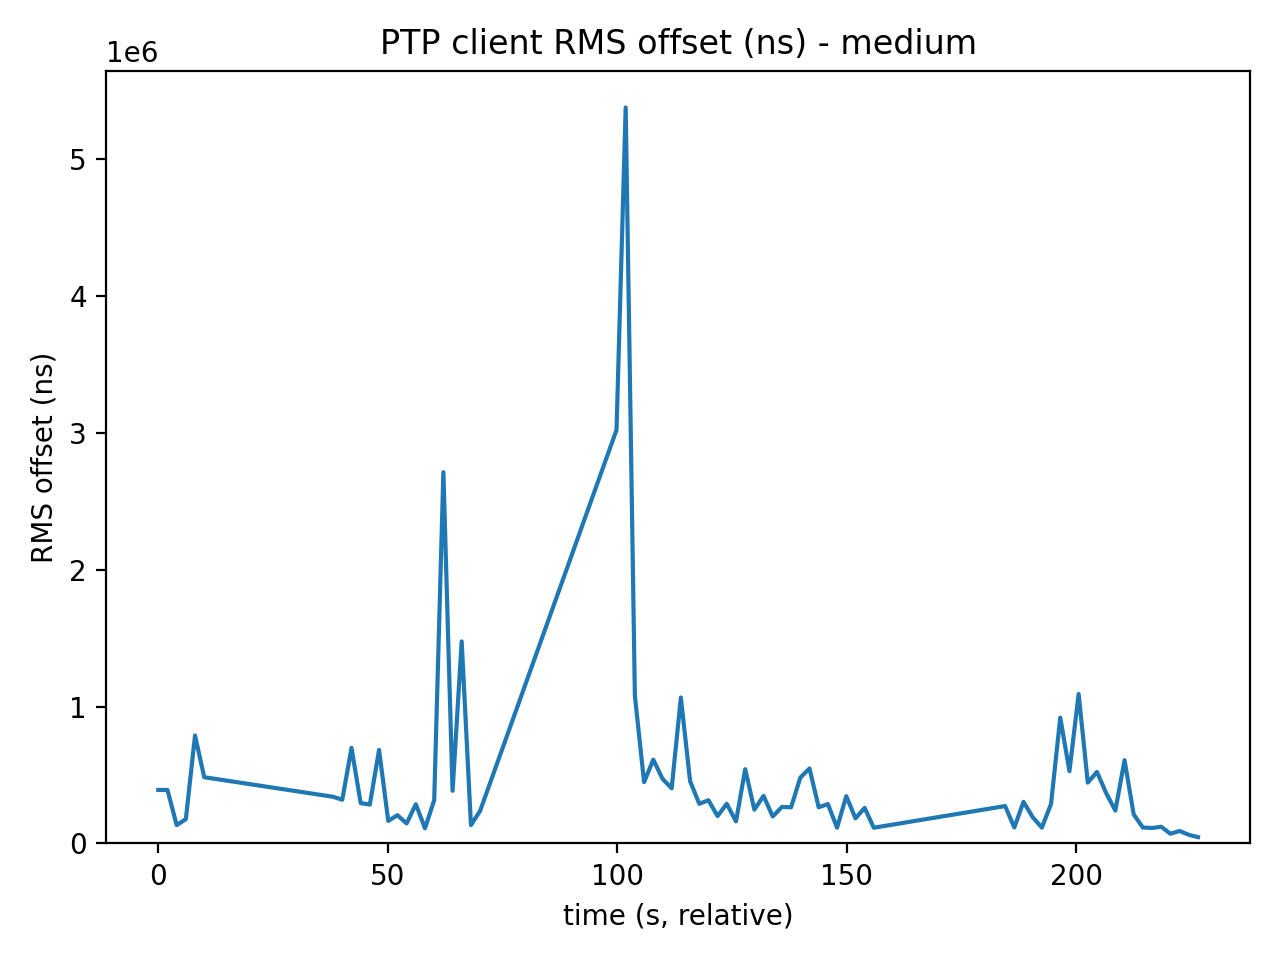
\includegraphics[width=\linewidth]{
      images/data_plots/plots_ptp/client_medium_rms_ns.png
    }
    \caption{Scenario MEDIUM}
  \end{subfigure}
  \caption{Comparazione della performance - nodo: \texttt{clientptp}}
  \label{fig:scenario_comparison}
\end{figure}

Nel caso \texttt{low}, l’\texttt{RMS offset} presenta una dinamica variabile ma
complessivamente contenuta. Il grafico mostra una serie oscillante attorno a valori
moderati, con numerosi picchi locali ma senza una tendenza persistente alla
crescita. Le statistiche confermano tale quadro: la media è pari a 333758.44 ns, la
mediana a 248869 ns e il terzo quartile a 367184.5 ns. La deviazione standard è
305485.19 ns, quindi elevata in valore assoluto ma ancora confrontabile con il livello
centrale della serie. Il massimo raggiunge 1643285 ns, a fronte di un minimo di 35456
ns; ciò indica la presenza di spike anche marcati, che però nel grafico rimangono
episodici e non ridefiniscono il comportamento prevalente della metrica. In
sostanza, nello scenario \texttt{low} il client mantiene un errore RMS
generalmente sotto controllo, pur con irregolarità non trascurabili.

Nel caso \texttt{medium}, il comportamento peggiora in modo evidente. La media
sale a 495222.80 ns, mentre la mediana aumenta a 289519 ns; cresce quindi sia il
livello medio sia il valore centrale della distribuzione. L’aspetto più rilevante
riguarda però la dispersione: la deviazione standard raggiunge 754809.35 ns e il
coefficiente di variazione è pari a 1.524, valore molto superiore a quello osservato
nello scenario \texttt{low} (0.915). Questo significa che la variabilità relativa
della metrica diventa estremamente elevata. Il grafico conferma chiaramente tale
instabilità, mostrando alcune escursioni molto pronunciate, tra cui un picco
massimo di 5374528 ns, nettamente superiore al massimo del caso \texttt{low}. Anche
l’intervallo interquartile cresce da 219077.5 ns a 293159.75 ns, segnalando che
l’aumento di dispersione non è dovuto soltanto a pochi valori anomali, ma interessa
più in generale l’intera distribuzione dei campioni.

Il confronto tra \texttt{low} e \texttt{medium} mostra quindi che l’\texttt{RMS
offset} del nodo \texttt{clientptp} è fortemente sensibile al peggioramento
delle condizioni sperimentali. Nel passaggio a \texttt{medium} non si osserva
soltanto un incremento dell’errore medio, ma soprattutto una perdita di stabilità
molto marcata, con spike ampi e una dispersione complessiva nettamente superiore.
Dal punto di vista sperimentale, questa metrica evidenzia quindi che il client
PTP, pur riuscendo ancora a produrre misure nello scenario intermedio, lo fa con
una qualità di sincronizzazione significativamente più degradata rispetto al
caso \texttt{low}. Nel caso \texttt{high}, infine, il degrado non si traduce in un
semplice ulteriore peggioramento quantitativo, ma nell’impossibilità stessa di
ottenere una serie RMS analizzabile.

\subsection{\texttt{boundary}}
L'analisi relativa al nodo \texttt{boundary} deve essere interpretata in modo differente
rispetto a quella del client. Le metriche osservate in questo caso descrivono
infatti il comportamento della sincronizzazione del boundary rispetto al \texttt{master
upstream (servergm)}, e non il collegamento downstram vero il \texttt{clientptp},
sul quale è stato introdotto il degrado di rete. Di conseguenza, in linea
teorica, non ci si attende un impatto diretto e strutturale degli impairment applicati
nei tre scenari sulle misure di offset e path delay rilevate sul boundary.

Occorre tuttavia considerare che il demone \texttt{ptp4l} opera sul nodo in modo
unitario, gestendo contemporaneamente più porte della topologia. Per questo
motivo, eventuali fault o transizioni di stato osservate sulla porta downstream possono
comunque rilfettersi indirettamente sulla stabilità complessiva del processo di sincronizzazione,
introducendo fluttazioni o anomalie anche nelle metriche riferite al tratto
upstream. L'analisi che segue è quindi finalizzata a verificare se i dati confermino
una sostanziale stabilitàdel boundary nei tre scenari oppure se emergano effetti indiretti
riconducibili alle criticità operative osservate durante il testing.

Per la metrica del offset saranno inoltre considerati sia i dati complessivi sia quelli
relativi alla sola fase \texttt{post-lock (servo\_state = s2)}.

\subsubsection{Analisi metrica: \texttt{path delay}}
\begin{figure}[H]
  \centering

  \begin{subfigure}
    {0.32\textwidth}
    \centering
    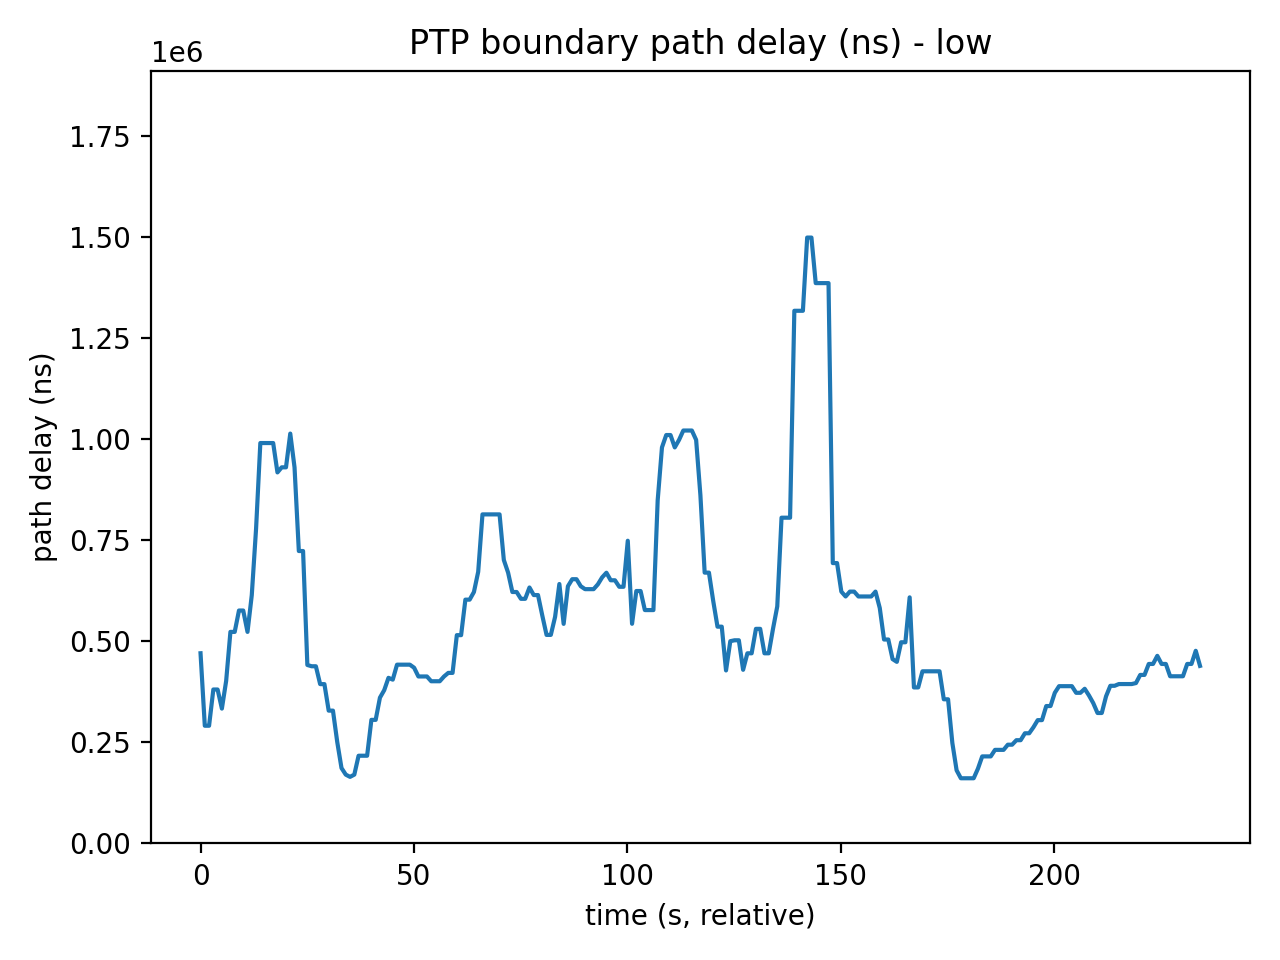
\includegraphics[width=\linewidth]{
      images/data_plots/plots_ptp/boundary_low_path_delay_ns.png
    }
    \caption{Scenario LOW}
  \end{subfigure}
  \hfill
  \begin{subfigure}
    {0.32\textwidth}
    \centering
    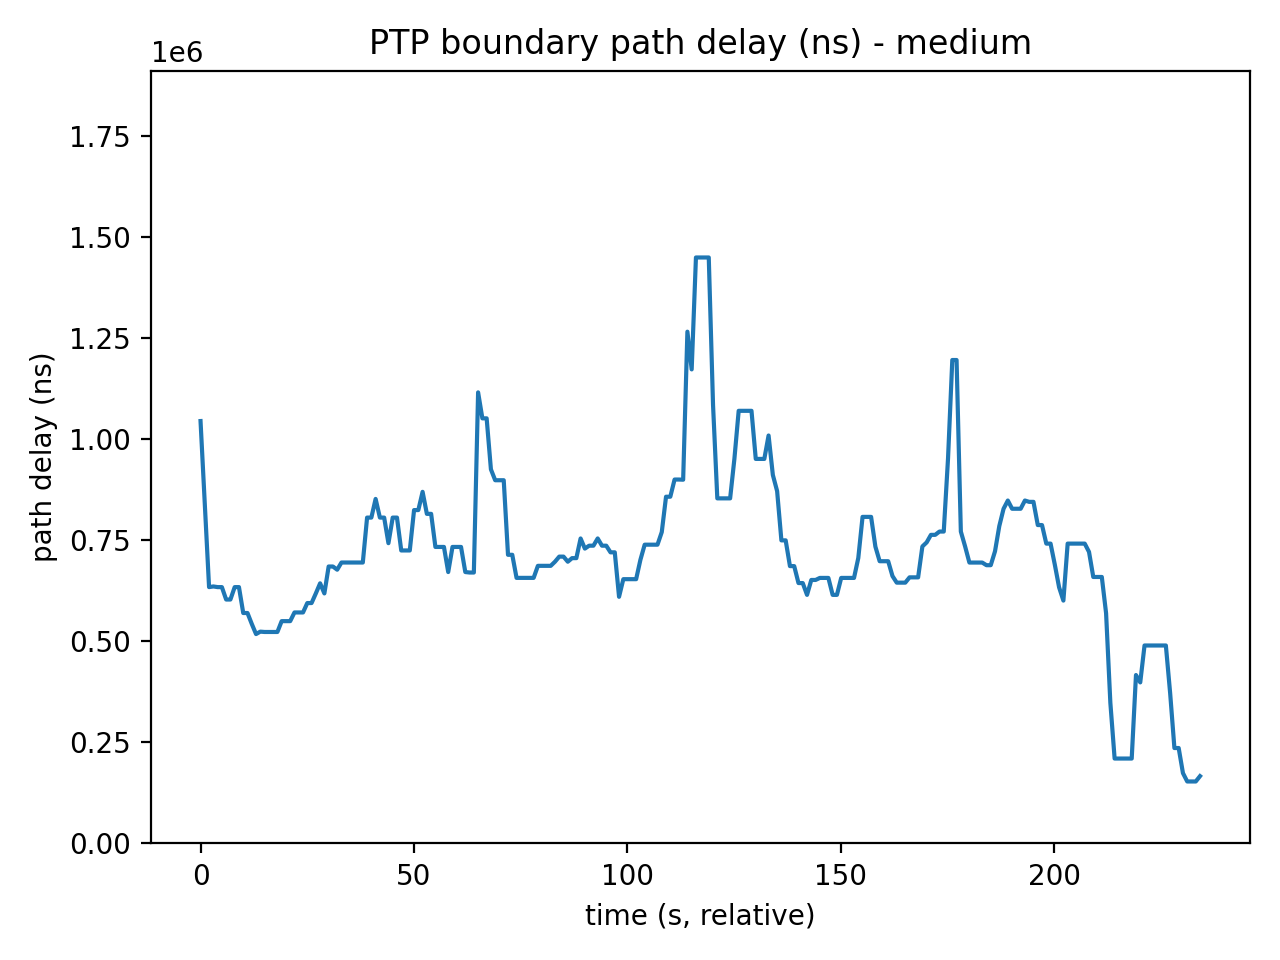
\includegraphics[width=\linewidth]{
      images/data_plots/plots_ptp/boundary_medium_path_delay_ns.png
    }
    \caption{Scenario MEDIUM}
  \end{subfigure}
  \begin{subfigure}
    {0.32\textwidth}
    \centering
    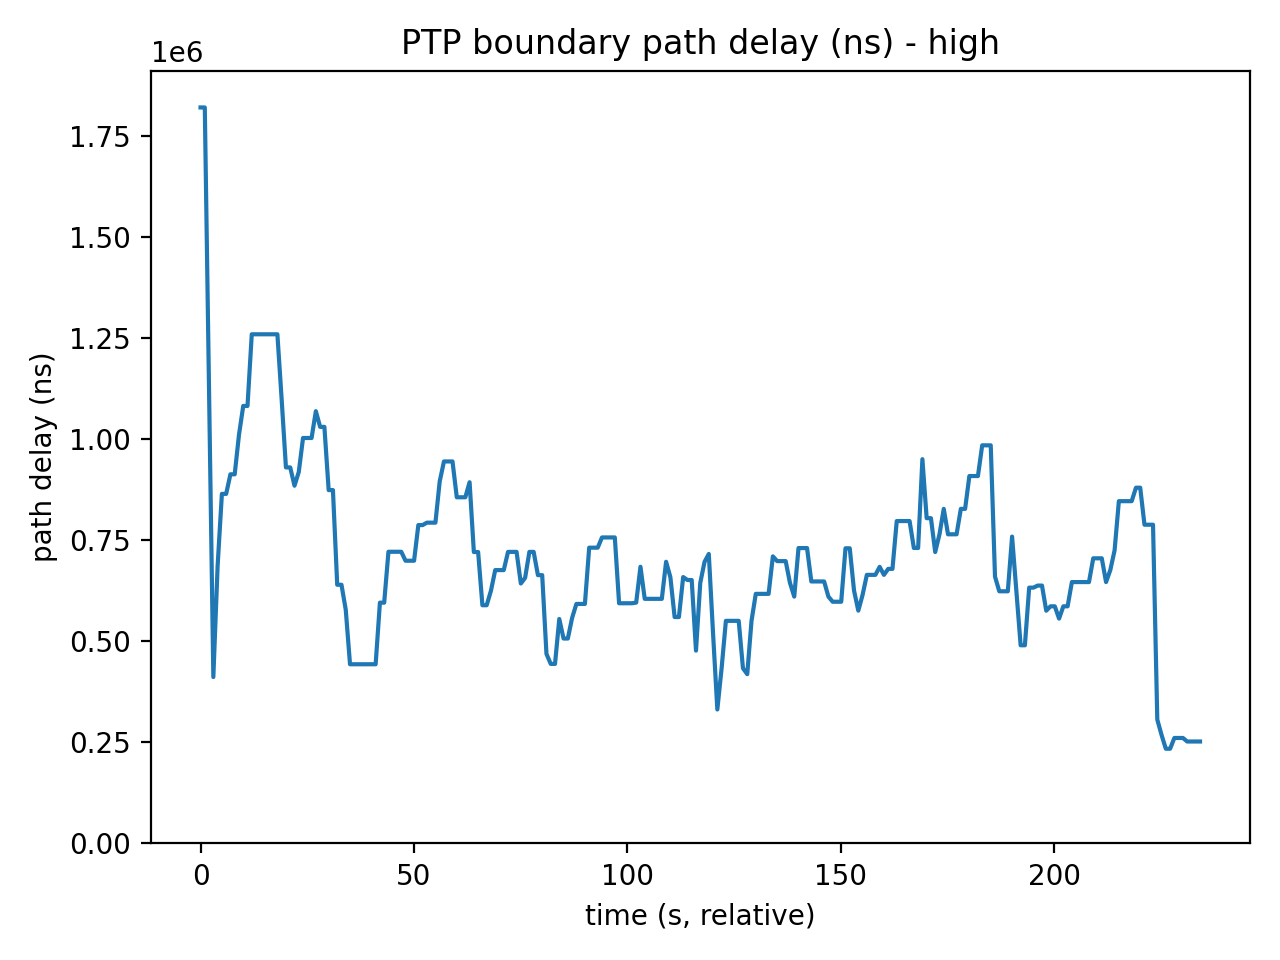
\includegraphics[width=\linewidth]{
      images/data_plots/plots_ptp/boundary_high_path_delay_ns.png
    }
    \caption{Scenario HIGH}
  \end{subfigure}
  \caption{Comparazione della performance - nodo: \texttt{boundary}}
  \label{fig:scenario_comparison}
\end{figure}
L’analisi del \texttt{path delay} del nodo \texttt{boundary} mostra delle
leggere differenze tra i tre scenari, ma non una crescita monotona e sistematica al
crescere dello stress di rete. Nello scenario \texttt{low} si osserva il valore centrale
più contenuto, con mediana pari a 476428 ns e media pari a 547340 ns; tuttavia,
la serie presenta una variabilità non trascurabile, con picchi fino a 1498267 ns,
che contribuiscono ad aumentare la media.

Nello scenario \texttt{medium} il livello centrale del \texttt{path delay}
aumenta, con mediana pari a 697914 ns e media pari a 714604 ns, mentre la
dispersione relativa risulta più contenuta rispetto al caso \texttt{low}, come
indicato da una deviazione standard di 208788 ns e da un coefficiente di
variazione pari a $0.292$.

Lo scenario \texttt{high} presenta valori centrali molto simili al caso \texttt{medium},
con mediana pari a 678988 ns e media pari a 707771 ns, ma mostra un massimo
superiore, pari a 1820002 ns, evidenziando la presenza di escursioni più marcate.

Nel complesso, i dati indicano che il \texttt{path delay} del \texttt{boundary} non
rimane perfettamente invariato tra gli scenari, ma l’effetto osservato consiste
soprattutto in un aumento del livello centrale passando da \texttt{low} a \texttt{medium},
mentre il passaggio da \texttt{medium} a \texttt{high} non produce un ulteriore incremento
stabile, bensì una maggiore presenza di valori estremi. L’andamento osservato non
conferma quindi una differenza strutturale nettamente attribuibile alle diverse condizioni
di rete, ma suggerisce piuttosto un’influenza di fattori secondari e della
variabilità interna delle misurazioni.

\subsubsection{Analisi metrica: \texttt{offset}}
\begin{figure}[H]
  \centering

  \begin{subfigure}
    {0.32\textwidth}
    \centering
    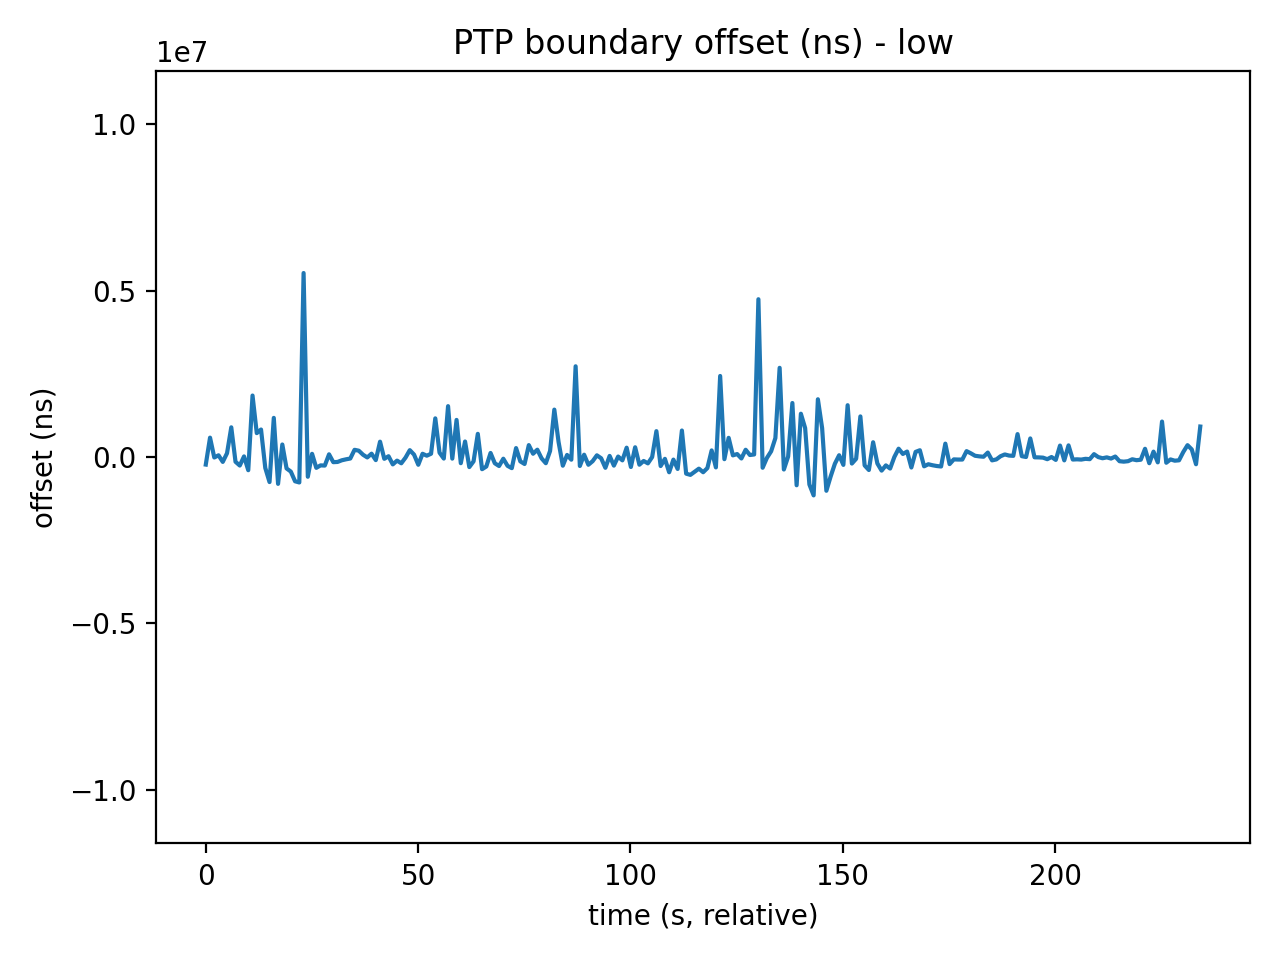
\includegraphics[width=\linewidth]{
      images/data_plots/plots_ptp/boundary_low_offset_ns.png
    }
    \caption{Scenario LOW}
  \end{subfigure}
  \hfill
  \begin{subfigure}
    {0.32\textwidth}
    \centering
    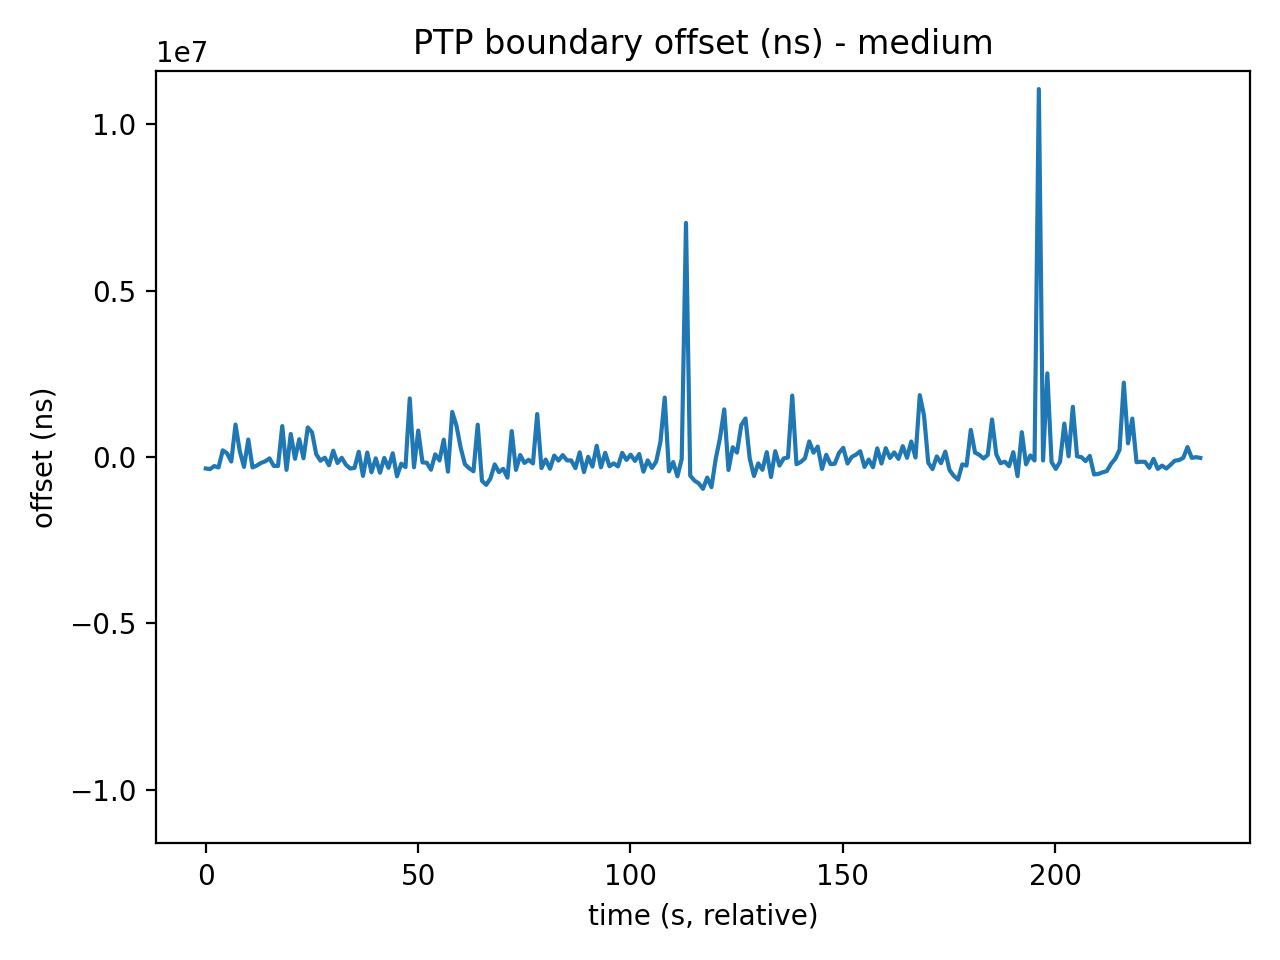
\includegraphics[width=\linewidth]{
      images/data_plots/plots_ptp/boundary_medium_offset_ns.png
    }
    \caption{Scenario MEDIUM}
  \end{subfigure}
  \begin{subfigure}
    {0.32\textwidth}
    \centering
    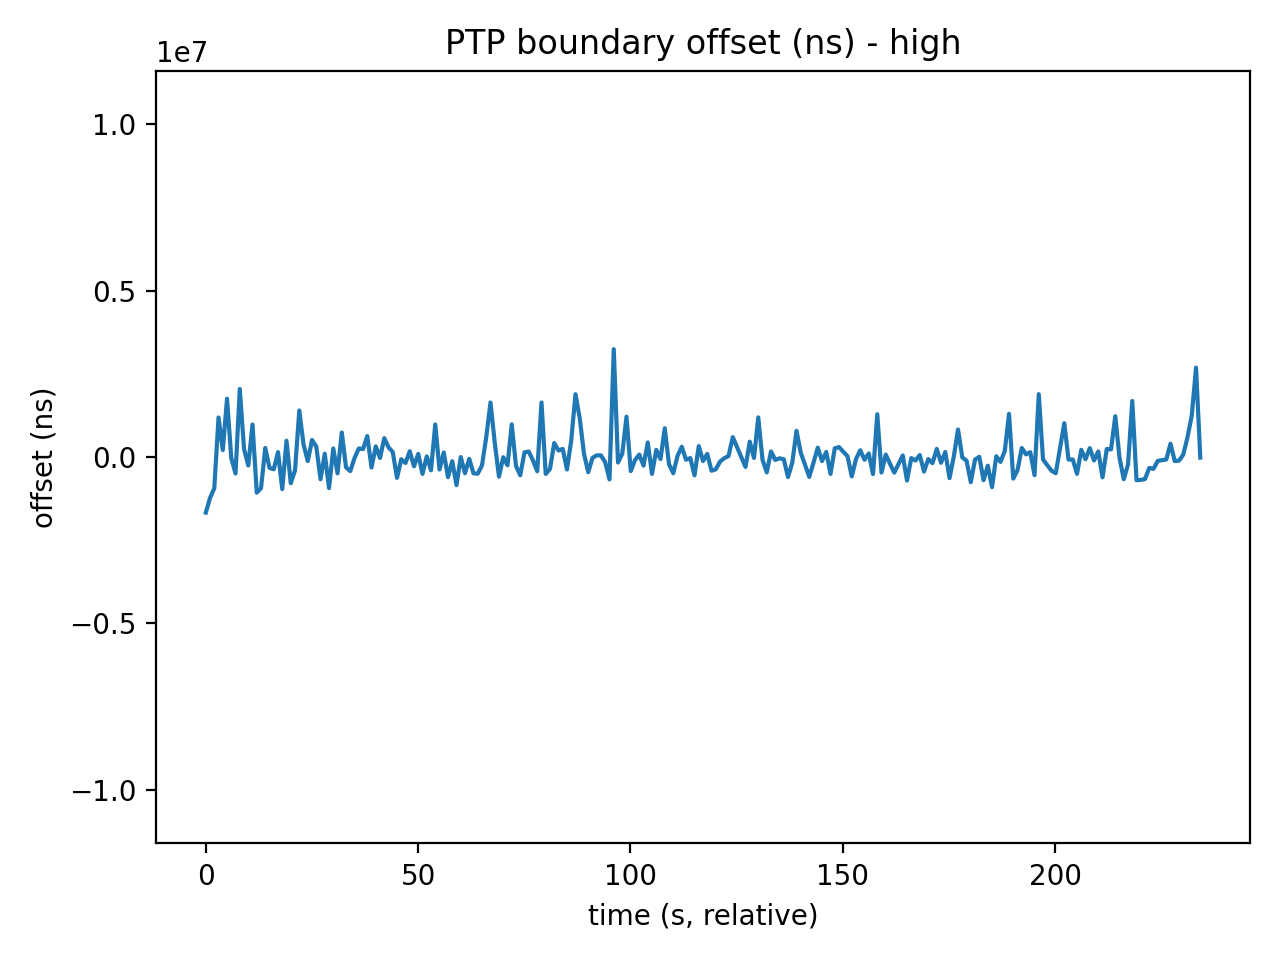
\includegraphics[width=\linewidth]{
      images/data_plots/plots_ptp/boundary_high_offset_ns.png
    }
    \caption{Scenario HIGH}
  \end{subfigure}
  \caption{Comparazione della performance - nodo: \texttt{boundary} - dati
  completi}
  \label{fig:scenario_comparison}
\end{figure}
\begin{figure}[H]
  \centering

  \begin{subfigure}
    {0.32\textwidth}
    \centering
    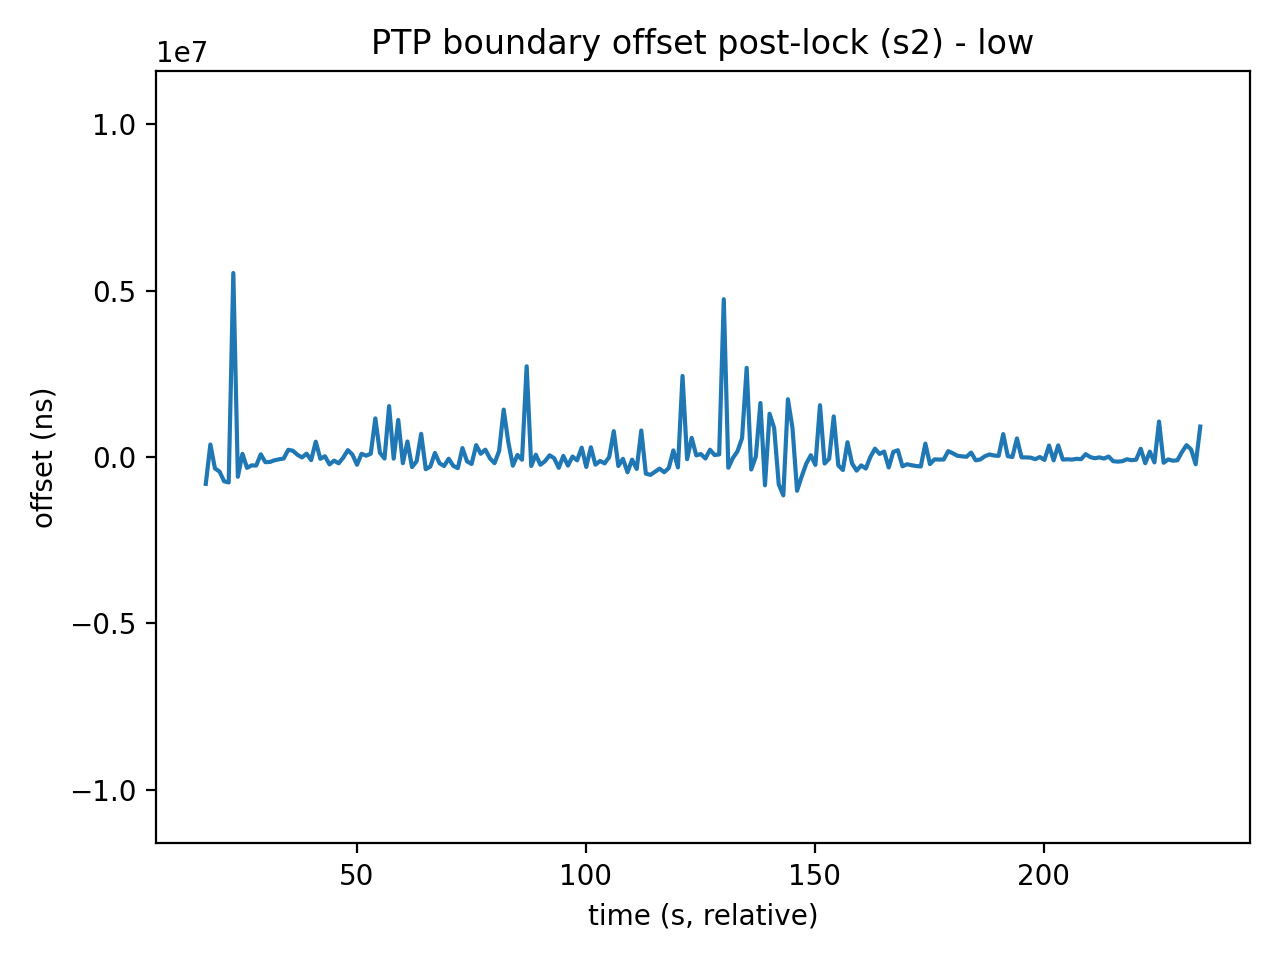
\includegraphics[width=\linewidth]{
      images/data_plots/plots_ptp/boundary_low_offset_ns_postlock_s2.png
    }
    \caption{Scenario LOW}
  \end{subfigure}
  \hfill
  \begin{subfigure}
    {0.32\textwidth}
    \centering
    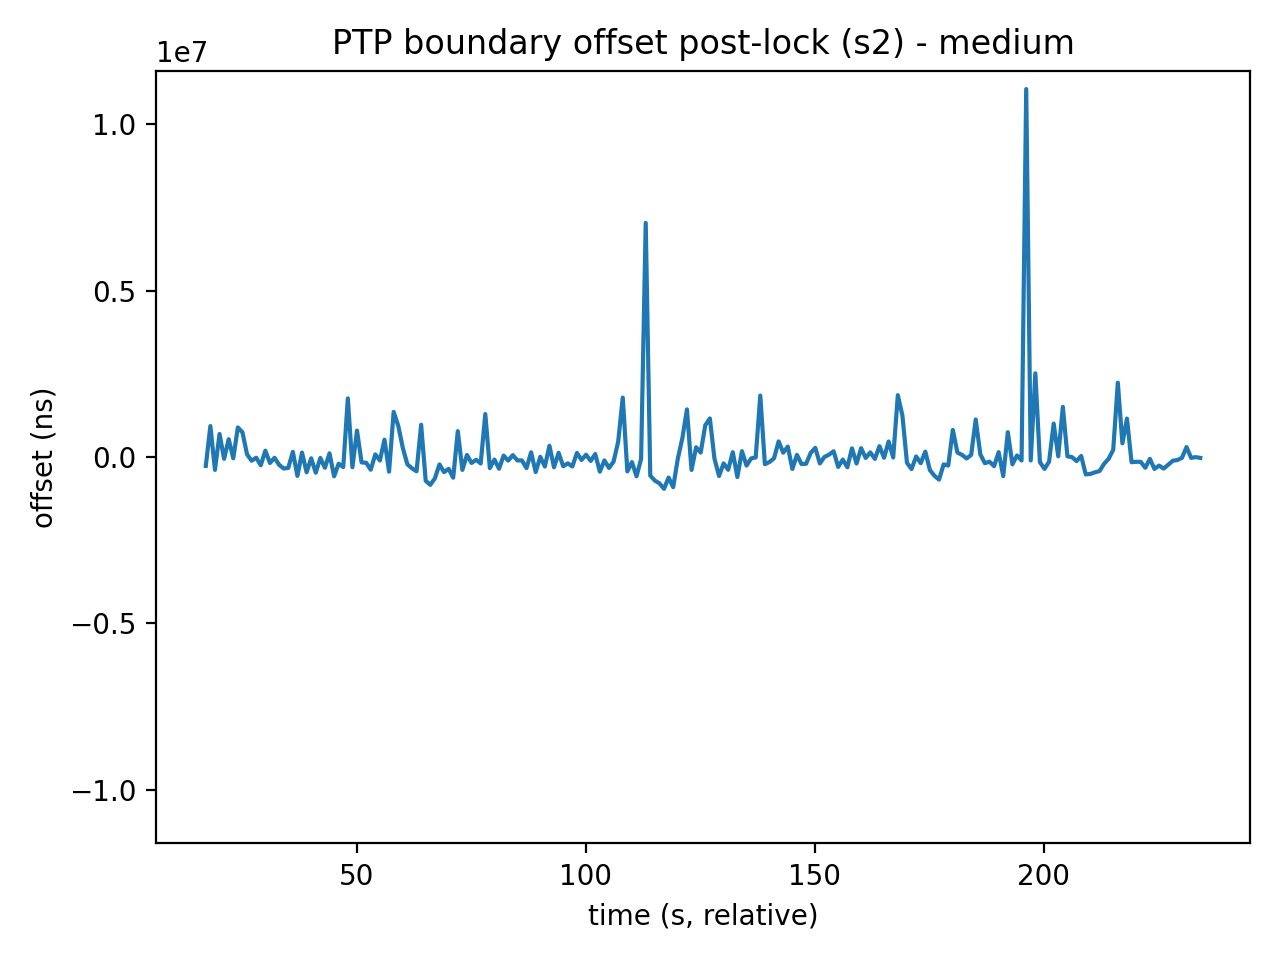
\includegraphics[width=\linewidth]{
      images/data_plots/plots_ptp/boundary_medium_offset_ns_postlock_s2.png
    }
    \caption{Scenario MEDIUM}
  \end{subfigure}
  \begin{subfigure}
    {0.32\textwidth}
    \centering
    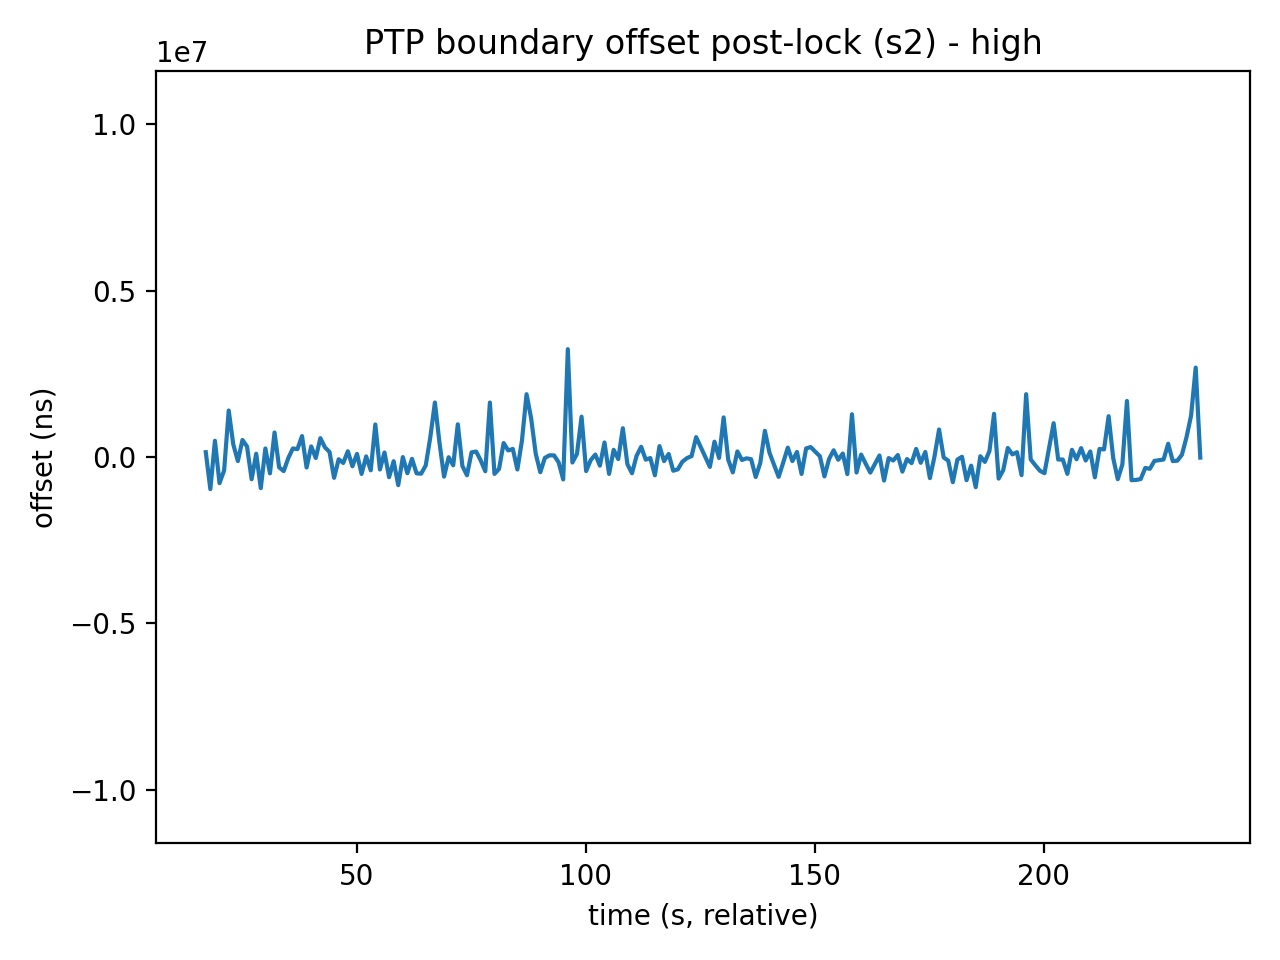
\includegraphics[width=\linewidth]{
      images/data_plots/plots_ptp/boundary_high_offset_ns_postlock_s2.png
    }
    \caption{Scenario HIGH}
  \end{subfigure}
  \caption{Comparazione della performance - nodo: \texttt{boundary} - dati
  filtrati: \texttt{servo\_state:s2}}
  \label{fig:scenario_comparison}
\end{figure}
L’analisi dell'\texttt{offset} del nodo \texttt{boundary}, considerato sia sull’intera
serie sia nel solo intervallo \texttt{post-lock} (\texttt{s2}), non evidenzia
una degradazione monotona al crescere dello stress di rete. In tutti e tre gli scenari
la distribuzione rimane infatti centrata in prossimità dello zero, con mediane
sempre leggermente negative: pari a $-43836$ ns in \texttt{low}, $-100004$ ns in \texttt{medium}
e $-59229$ ns in \texttt{high}. Anche limitando l’osservazione alla sola fase
\texttt{post-lock}, il quadro resta sostanzialmente invariato, con mediane pari rispettivamente
a $-45273.5$ ns, $-88836.5$ ns e $-56328.5$ ns.

Le differenze principali tra gli scenari riguardano soprattutto la presenza di
escursioni impulsive. Lo scenario \texttt{medium} è quello che mostra gli eventi
più estremi, con massimo pari a $11064269$ ns e deviazione standard pari a $10078
06$ ns sull’intera serie, valori che rimangono elevati anche nel \texttt{post-lock}.
Lo scenario \texttt{low} presenta picchi meno pronunciati, ma comunque rilevanti,
fino a $5533287$ ns, mentre lo scenario \texttt{high} mostra massimi inferiori rispetto
a \texttt{medium}, pari a $3244309$ ns, pur mantenendo una dispersione centrale
non trascurabile, come indicato dall’\texttt{IQR} più ampio tra i tre casi.

Il confronto tra serie complete e serie \texttt{post-lock} mostra inoltre che
l’esclusione della fase iniziale di acquisizione del sincronismo modifica solo
in misura limitata gli indicatori descrittivi. Ciò suggerisce che la variabilità dell’\texttt{offset}
non sia concentrata esclusivamente nella fase transitoria, ma permanga anche
durante il funzionamento stabilizzato del servo, sotto forma di oscillazioni attorno
allo zero e di sporadici valori anomali.

Nel complesso, i dati non confermano una differenza sistematica dell’\texttt{offset}
attribuibile alle diverse condizioni di rete imposte nei tre scenari. L’effetto osservato
appare piuttosto dominato da fluttuazioni locali e da picchi isolati, più che da
un peggioramento strutturale e progressivo associato all’aumento dello stress di
rete.

\section{\texttt{chronyd}}
Nel caso di \texttt{Chrony}, l’analisi è stata svolta su una topologia composta
dal solo collegamento tra \texttt{servergm} e \texttt{clientchrony}, senza la presenza
di nodi \texttt{boundary}. In questo contesto, il degrado di rete tramite
\texttt{tc}/\texttt{netem} è stato applicato in due configurazioni distinte: in un
primo caso sull’interfaccia del \texttt{clientchrony}, in un secondo caso sull’interfaccia
del \texttt{servergm}.

Questa doppia configurazione consente di osservare separatamente gli effetti del
degrado introdotto lungo le due direzioni logiche della comunicazione tra client
e server. Poiché il meccanismo di sincronizzazione di \texttt{Chrony} si basa
sullo scambio di messaggi tra i due estremi, applicare l’alterazione su un lato oppure
sull’altro permette di valutare se il posizionamento del disturbo lungo il percorso
influenzi in modo differente le metriche osservate.

Nel seguito verranno quindi confrontati non solo i diversi livelli di stress di rete,
ma anche i risultati ottenuti nelle due configurazioni di applicazione del
degrado. È inoltre opportuno precisare che tutte le metriche analizzate sono state
rilevate esclusivamente tramite interrogazione del nodo \texttt{clientchrony}, poiché
è da esso che si ricavano le misure direttamente rilevanti per valutare la qualità
della sincronizzazione dal punto di vista del client.

\subsection{Analisi metrica: \texttt{offset}}
\begin{figure}[H]
  \centering

  \begin{subfigure}
    {0.32\textwidth}
    \centering
    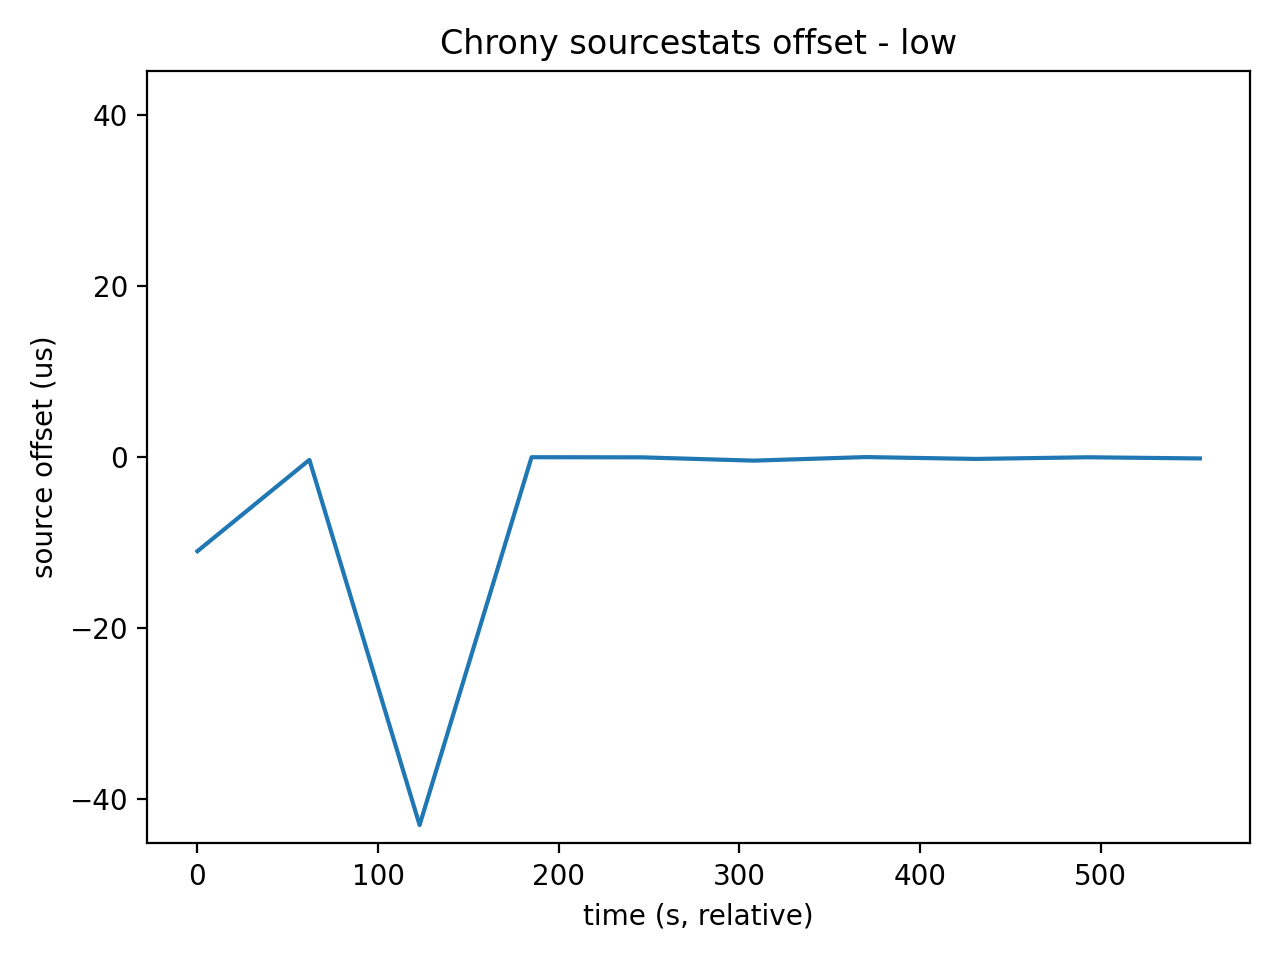
\includegraphics[width=\linewidth]{
      images/data_plots/plots_chrony_clientchrony/chrony_low_sourcestats_offset_us.png
    }
    \caption{Scenario LOW}
  \end{subfigure}
  \hfill
  \begin{subfigure}
    {0.32\textwidth}
    \centering
    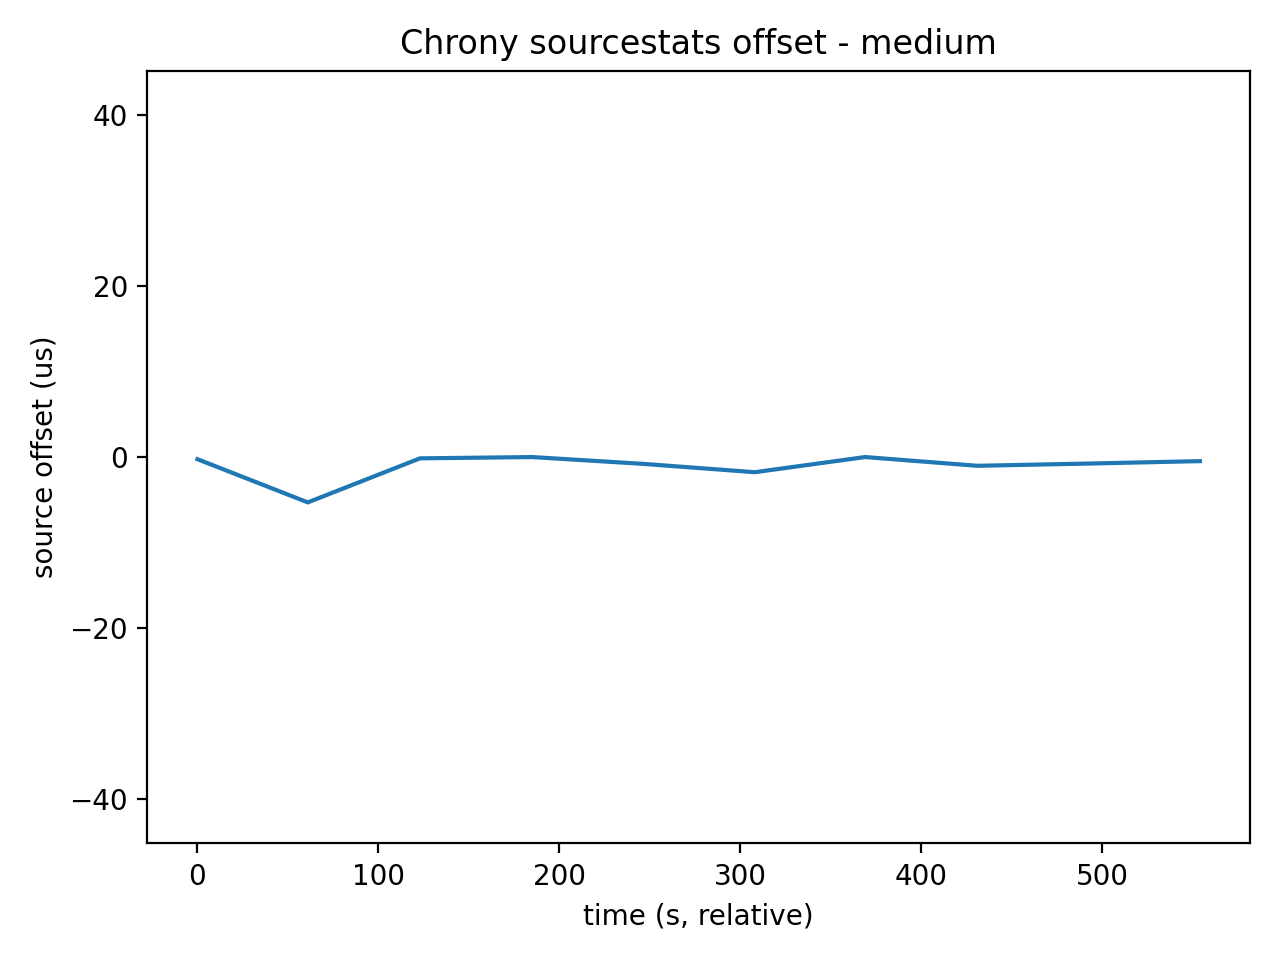
\includegraphics[width=\linewidth]{
      images/data_plots/plots_chrony_clientchrony/chrony_medium_sourcestats_offset_us.png
    }
    \caption{Scenario MEDIUM}
  \end{subfigure}
  \begin{subfigure}
    {0.32\textwidth}
    \centering
    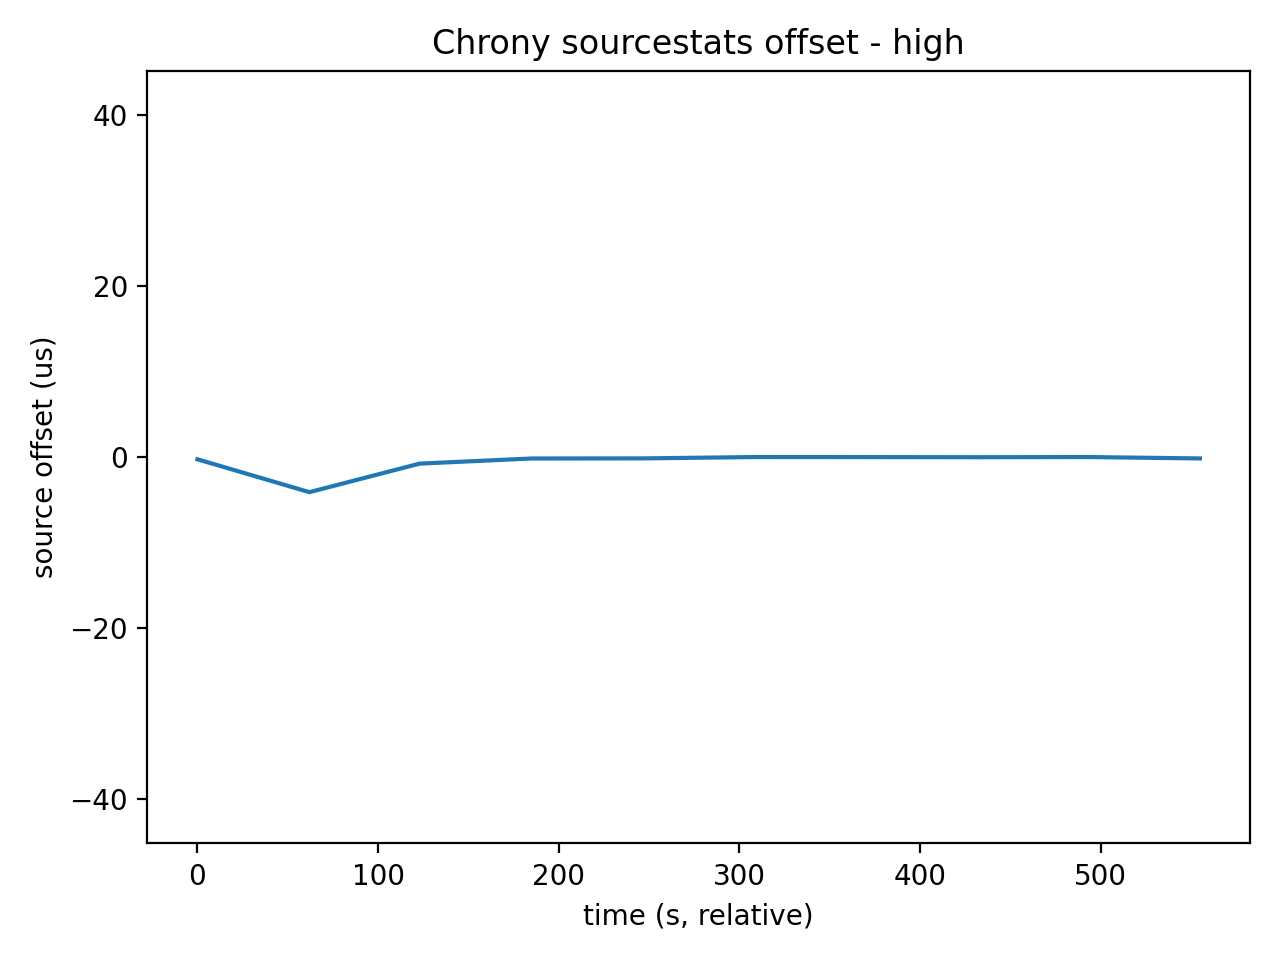
\includegraphics[width=\linewidth]{
      images/data_plots/plots_chrony_clientchrony/chrony_high_sourcestats_offset_us.png
    }
    \caption{Scenario HIGH}
  \end{subfigure}
  \caption{Comparazione della performance - nodo: \texttt{clientchrony} - netem/tc:
  \texttt{clientchrony}}
  \label{fig:scenario_comparison}
\end{figure}
\begin{figure}[H]
  \centering

  \begin{subfigure}
    {0.32\textwidth}
    \centering
    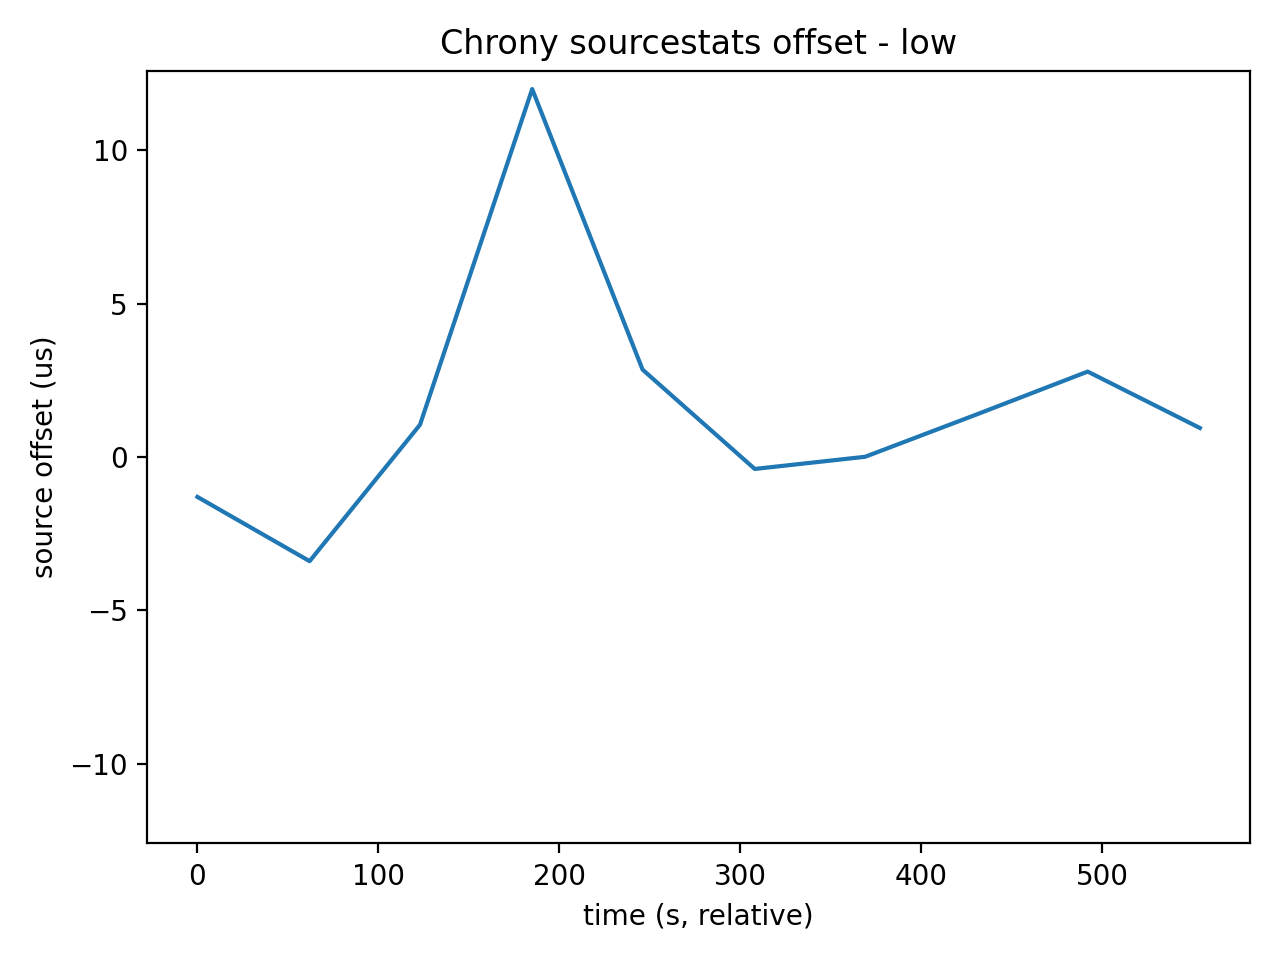
\includegraphics[width=\linewidth]{
      images/data_plots/plots_chrony_servergm/chrony_low_sourcestats_offset_us.png
    }
    \caption{Scenario LOW}
  \end{subfigure}
  \hfill
  \begin{subfigure}
    {0.32\textwidth}
    \centering
    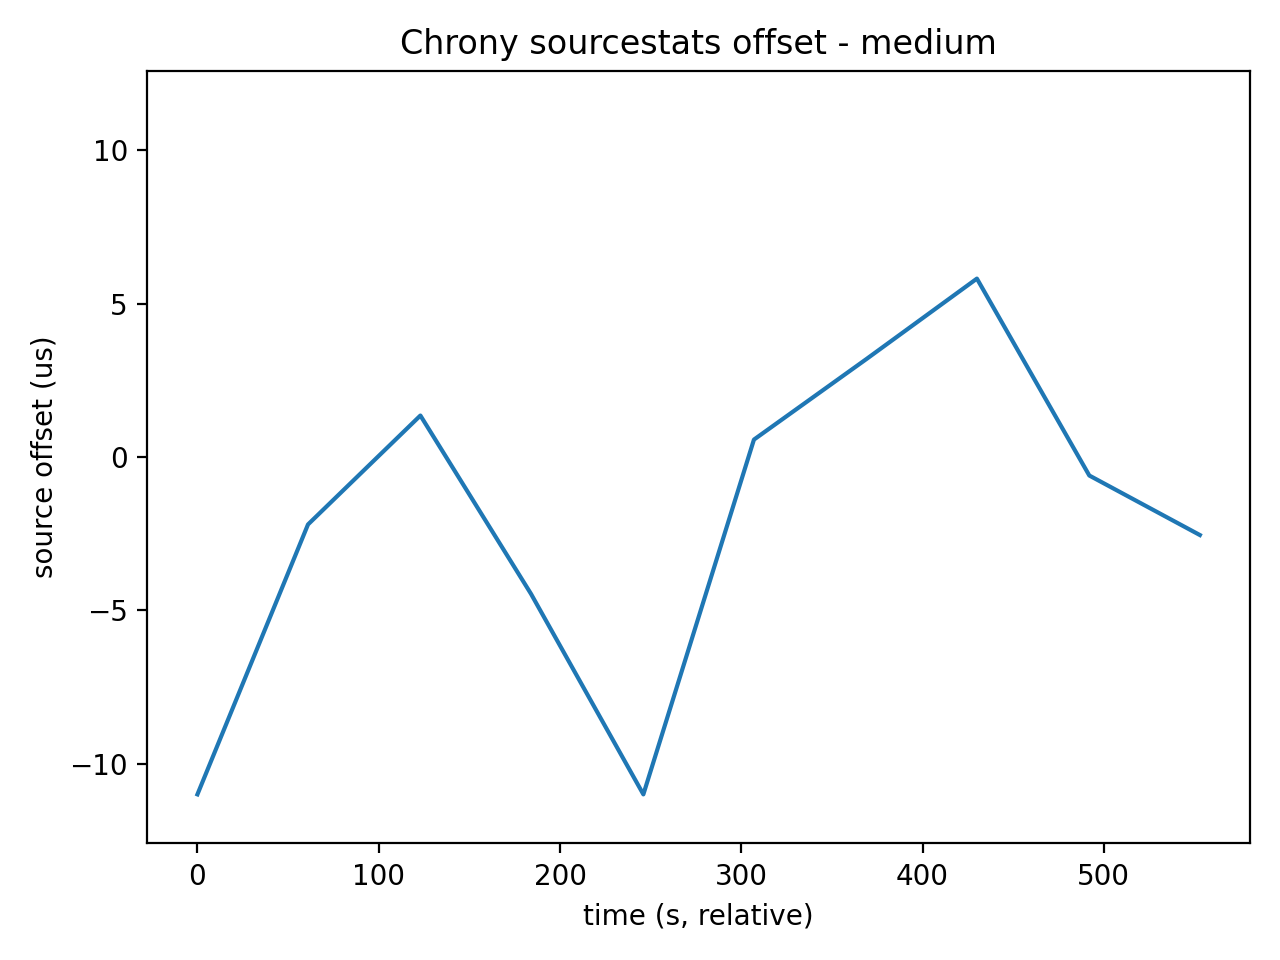
\includegraphics[width=\linewidth]{
      images/data_plots/plots_chrony_servergm/chrony_medium_sourcestats_offset_us.png
    }
    \caption{Scenario MEDIUM}
  \end{subfigure}
  \begin{subfigure}
    {0.32\textwidth}
    \centering
    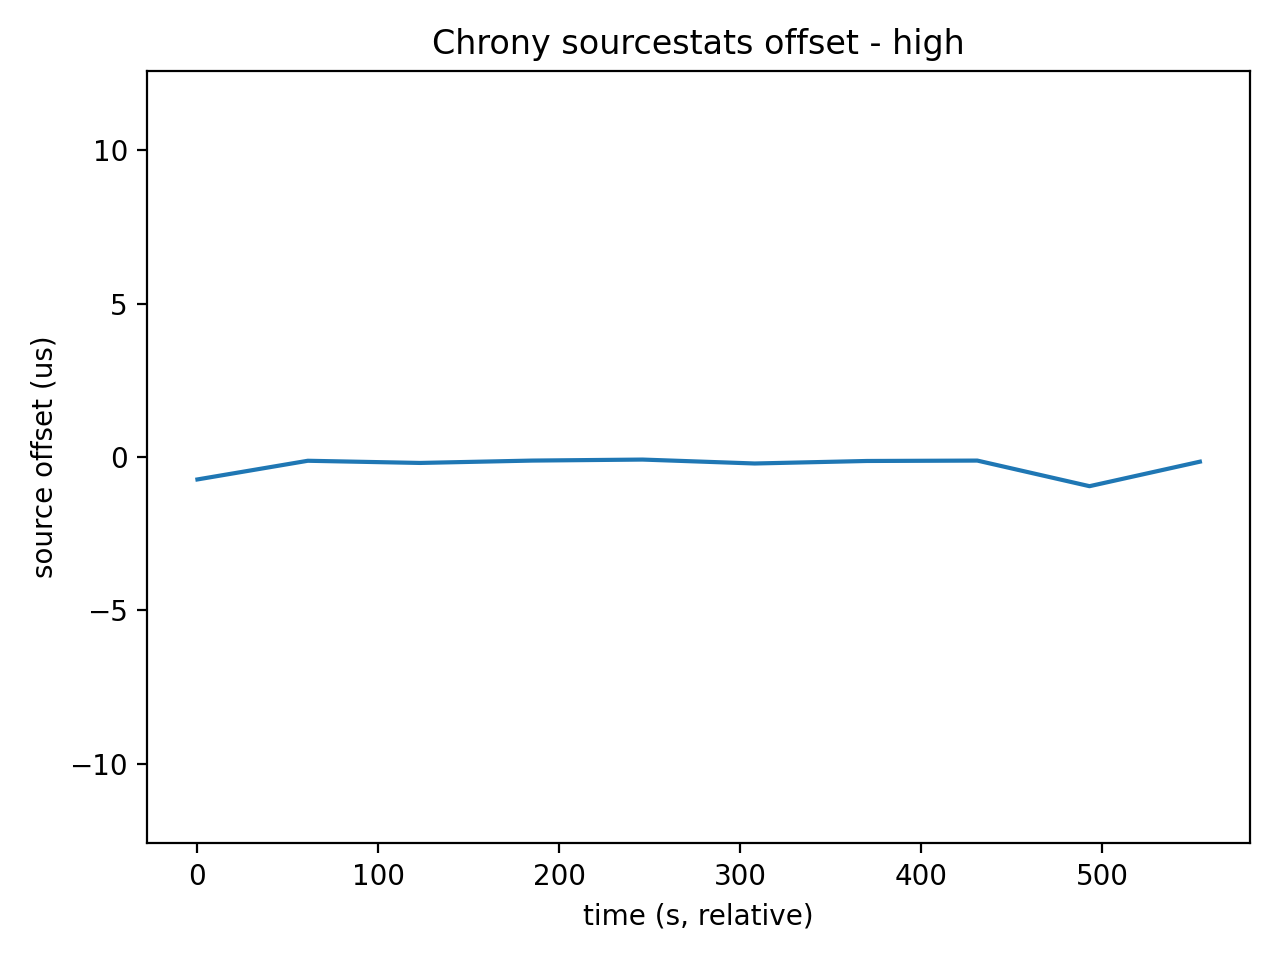
\includegraphics[width=\linewidth]{
      images/data_plots/plots_chrony_servergm/chrony_high_sourcestats_offset_us.png
    }
    \caption{Scenario HIGH}
  \end{subfigure}
  \caption{Comparazione della performance - nodo: \texttt{clientchrony} - netem/tc:
  \texttt{servergm}}
  \label{fig:scenario_comparison}
\end{figure}
\paragraph*{clientchrony - netem/tc:}
L’analisi dell’\texttt{offset} ottenuto tramite \texttt{chronyc sourcestats},
nel caso in cui il degrado di rete sia applicato sul lato \texttt{clientChrony},
mostra un comportamento complessivamente stabile in tutti e tre gli scenari
considerati. In termini temporali, dopo una possibile escursione iniziale, i valori
si mantengono molto prossimi allo zero per tutta la durata dell’osservazione,
senza evidenziare derive progressive né oscillazioni ampie e persistenti.

Dal punto di vista quantitativo, nello scenario \texttt{low} si osserva la
maggiore anomalia puntuale, con un minimo pari a $-43.0\,\mu s$, che influenza
in modo marcato media e variabilità campionaria; infatti la media risulta pari a $-
5.52\,\mu s$ e la deviazione standard a $13.60\,\mu s$. Tuttavia, il grafico mostra
che tale comportamento è riconducibile a un singolo campione isolato, mentre i
restanti valori si dispongono in prossimità dello zero.

Negli scenari \texttt{medium} e \texttt{high} il comportamento risulta ancora
più regolare. Nel caso \texttt{medium} la media è pari a $-1.05\,\mu s$, con mediana
$-0.62\,\mu s$ e minimo $-5.30\,\mu s$; nel caso \texttt{high} la media è $-0.56\,
\mu s$, con mediana $-0.16\,\mu s$ e minimo $-4.10\,\mu s$. In entrambi i casi,
la serie temporale rimane vicina allo zero lungo tutto l’intervallo osservato, senza
mostrare un peggioramento sistematico all’aumentare dello stress di rete.

Nel complesso, i dati non evidenziano differenze strutturali tra i tre scenari
per questa metrica. L’\texttt{offset} stimato da \texttt{sourcestats} resta
infatti contenuto e sostanzialmente stabile anche al crescere del degrado
applicato sul \texttt{client}, mentre l’unica deviazione rilevante compare nel
caso \texttt{low} come evento isolato e non come effetto sistematico delle condizioni
di rete.

\paragraph*{servergm - netem/tc:}
L’analisi dell’\texttt{offset} rilevato tramite \texttt{chronyc sourcestats},
nel caso in cui il degrado di rete sia applicato sul nodo \texttt{servergm},
evidenzia un comportamento differente nei tre scenari, ma senza una tendenza lineare
univoca al crescere dello stress.

Nello scenario \texttt{low} i valori risultano piuttosto dispersi e comprendono
sia campioni negativi sia positivi, con media pari a $1.596~\mu s$, mediana pari
a $1 .001~\mu s$ e massimo pari a $12.0~\mu s$. Il grafico mostra infatti una dinamica
irregolare, caratterizzata da un picco positivo pronunciato nella parte centrale
della serie, che incide in modo evidente sul valore medio.

Nello scenario \texttt{medium} permane una variabilità apprezzabile, ma con centro
della distribuzione spostato in campo negativo: la media è pari a
$-2.087~ \mu s$ e la mediana a $-1.4~\mu s$, con valori compresi tra $-11.0~\mu s$
e $5.819~\mu s$. Anche in questo caso la serie non mostra stabilità attorno a un
livello costante, ma alterna scostamenti di segno opposto con ampiezza non trascurabile.

Lo scenario \texttt{high} presenta invece un andamento nettamente più compatto. I
campioni restano tutti prossimi allo zero e interamente in campo negativo, con
media pari a $-0.279~\mu s$, mediana pari a $-0.140~\mu s$ e deviazione standard pari
a $0.302~\mu s$, molto inferiore rispetto ai casi \texttt{low} e \texttt{medium}.
Anche dal grafico emerge una serie quasi piatta, con oscillazioni molto
contenute e assenza di picchi rilevanti.

Nel complesso, i dati non mostrano un peggioramento progressivo dell’\texttt{offset}
all’aumentare dello stress di rete. Al contrario, il caso \texttt{high} risulta
il più regolare tra i tre, mentre le maggiori escursioni si osservano negli scenari
\texttt{low} e \texttt{medium}. Pertanto, anche in questo caso non emerge una relazione
diretta e sistematica tra intensità del degrado applicato su \texttt{servergm} e
aumento dell’\texttt{offset} misurato sul client.

\paragraph*{Confronto:}
Confrontando i due casi di applicazione del degrado di rete, ossia sul nodo
\texttt{clientchrony} e sul nodo \texttt{servergm}, emerge che l’\texttt{offset} misurato
tramite \texttt{chronyc sourcestats} rimane in generale contenuto in entrambi i
contesti, ma con differenze apprezzabili in termini di regolarità e sensibilità agli
scenari.

Nel caso in cui il degrado sia applicato su \texttt{clientchrony}, i valori dell’\texttt{offset}
risultano quasi sempre molto prossimi allo zero nei tre scenari, con scostamenti
medi pari a $-5.521~\mu s$ in \texttt{low}, $-1.051~\mu s$ in \texttt{medium} e $-
0.564~\mu s$ in \texttt{high}. A parte un singolo campione anomalo nello scenario
\texttt{low} e oscillazioni moderate nel caso \texttt{medium}, l’andamento
osservato è sostanzialmente stabile e non mostra variazioni strutturali
rilevanti al crescere dello stress.

Quando invece il degrado è applicato su \texttt{servergm}, la serie appare in
media più irregolare negli scenari \texttt{low} e \texttt{medium}. In particolare,
nello scenario \texttt{low} si osservano escursioni fino a $12.0~\mu s$, mentre
nel caso \texttt{medium} i valori variano tra $-11.0~\mu s$ e $5.819~\mu s$.
Solo nello scenario \texttt{high} il comportamento torna ad essere molto compatto,
con valori tutti vicini allo zero e deviazione standard pari a $0.302~\mu s$.

Nel confronto diretto, quindi, l’applicazione del degrado sul lato \texttt{clientchrony}
produce un comportamento complessivamente più stabile e più uniforme tra i tre scenari,
mentre l’applicazione su \texttt{servergm} introduce una maggiore variabilità nei
casi \texttt{low} e \texttt{medium}. Tuttavia, in nessuno dei due contesti emerge
una crescita monotona dell’\texttt{offset} al crescere dello stress di rete. Di
conseguenza, anche il confronto tra le due modalità di applicazione del \texttt{netem}
non evidenzia un effetto sistematico delle condizioni di rete su questa metrica, ma
piuttosto differenze di stabilità locale tra le due configurazioni sperimentali.

\subsection{Analisi metrica: \texttt{stddev}}
\begin{figure}[H]
  \centering

  \begin{subfigure}
    {0.32\textwidth}
    \centering
    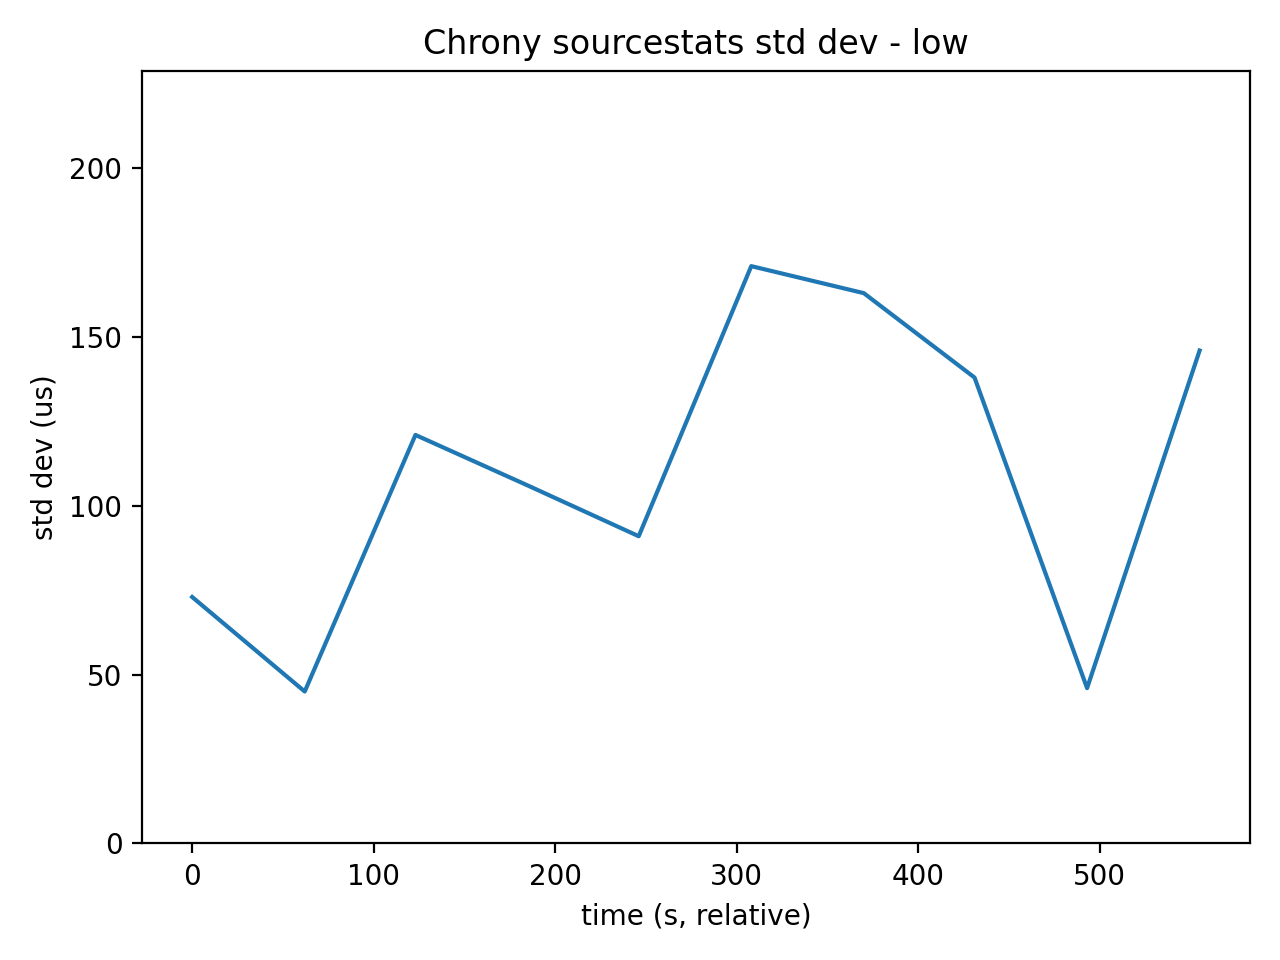
\includegraphics[width=\linewidth]{
      images/data_plots/plots_chrony_clientchrony/chrony_low_sourcestats_stddev_us.png
    }
    \caption{Scenario LOW}
  \end{subfigure}
  \hfill
  \begin{subfigure}
    {0.32\textwidth}
    \centering
    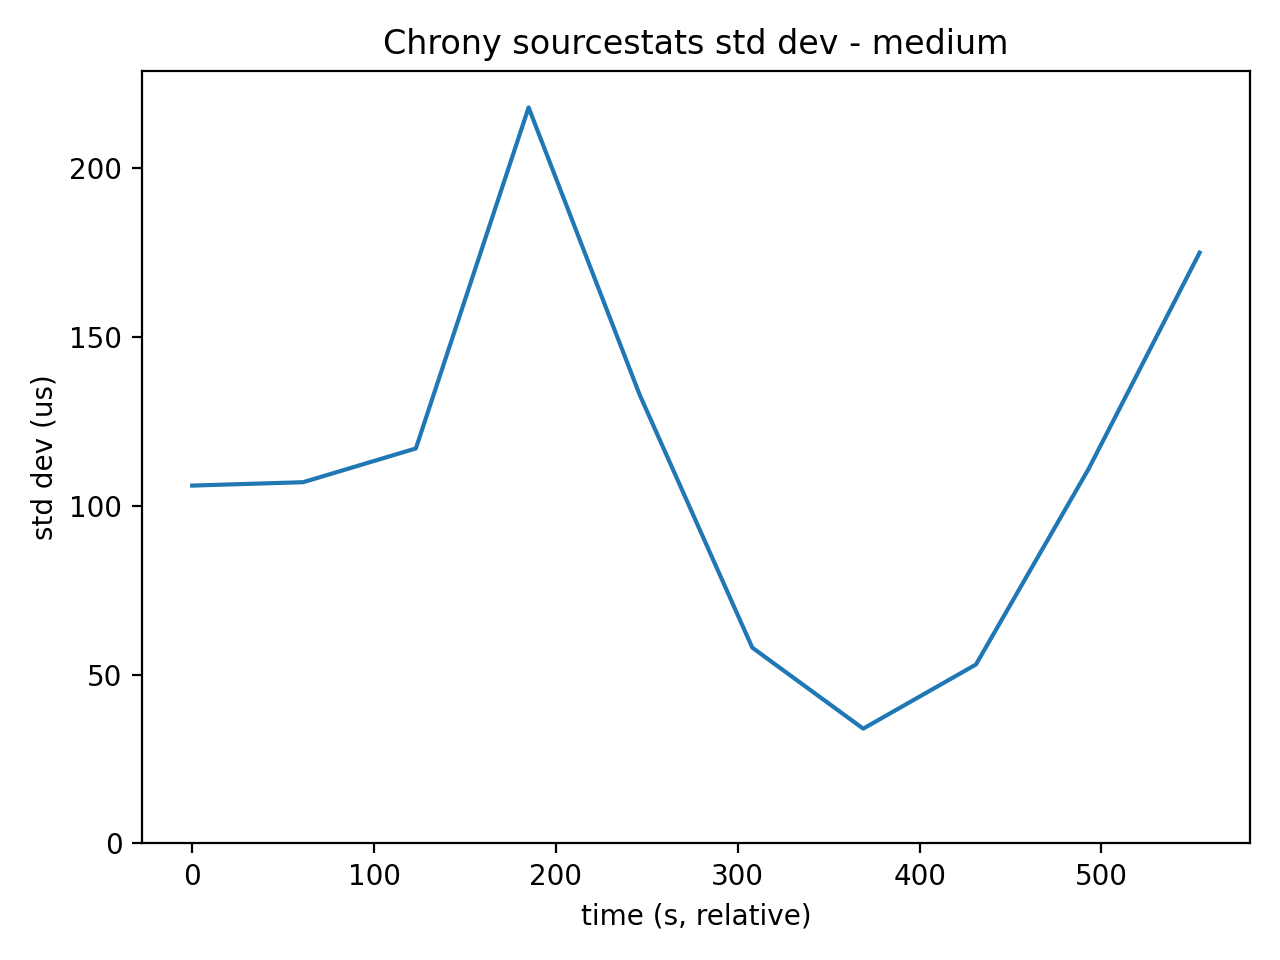
\includegraphics[width=\linewidth]{
      images/data_plots/plots_chrony_clientchrony/chrony_medium_sourcestats_stddev_us.png
    }
    \caption{Scenario MEDIUM}
  \end{subfigure}
  \begin{subfigure}
    {0.32\textwidth}
    \centering
    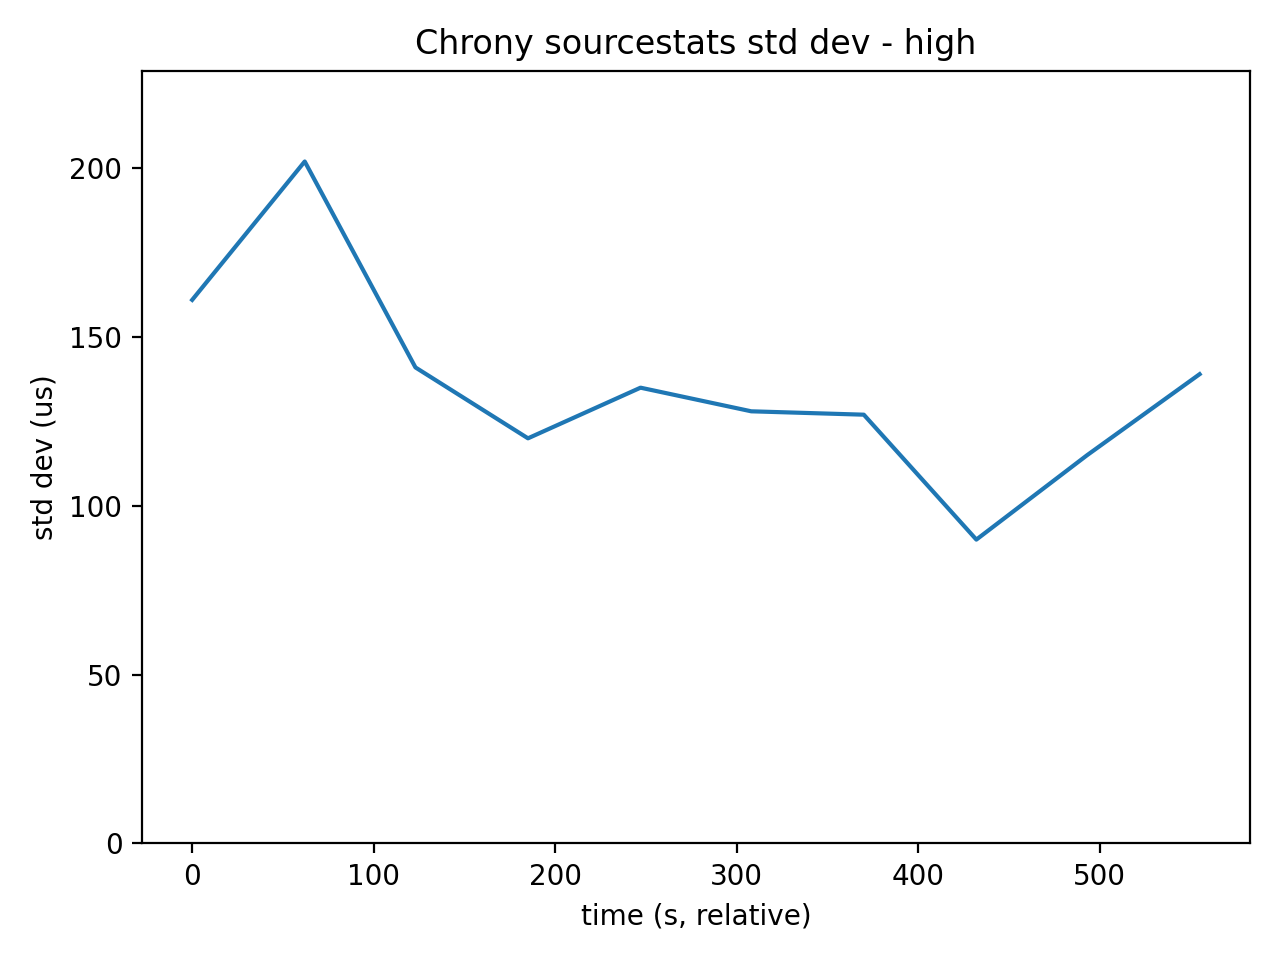
\includegraphics[width=\linewidth]{
      images/data_plots/plots_chrony_clientchrony/chrony_high_sourcestats_stddev_us.png
    }
    \caption{Scenario HIGH}
  \end{subfigure}
  \caption{Comparazione della performance - nodo: \texttt{clientchrony} - netem/tc:
  \texttt{clientchrony}}
  \label{fig:scenario_comparison}
\end{figure}
\begin{figure}[H]
  \centering

  \begin{subfigure}
    {0.32\textwidth}
    \centering
    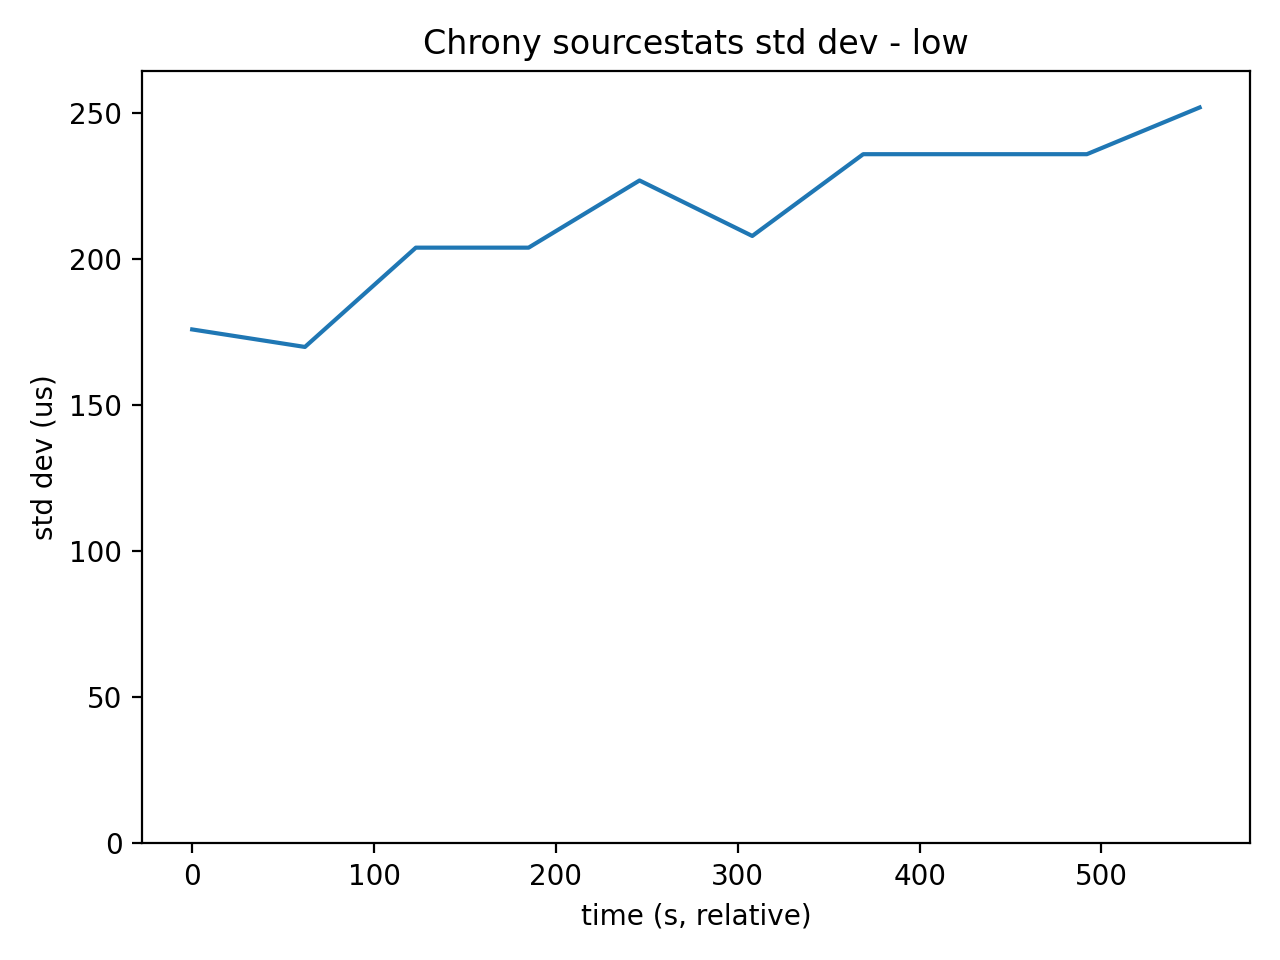
\includegraphics[width=\linewidth]{
      images/data_plots/plots_chrony_servergm/chrony_low_sourcestats_stddev_us.png
    }
    \caption{Scenario LOW}
  \end{subfigure}
  \hfill
  \begin{subfigure}
    {0.32\textwidth}
    \centering
    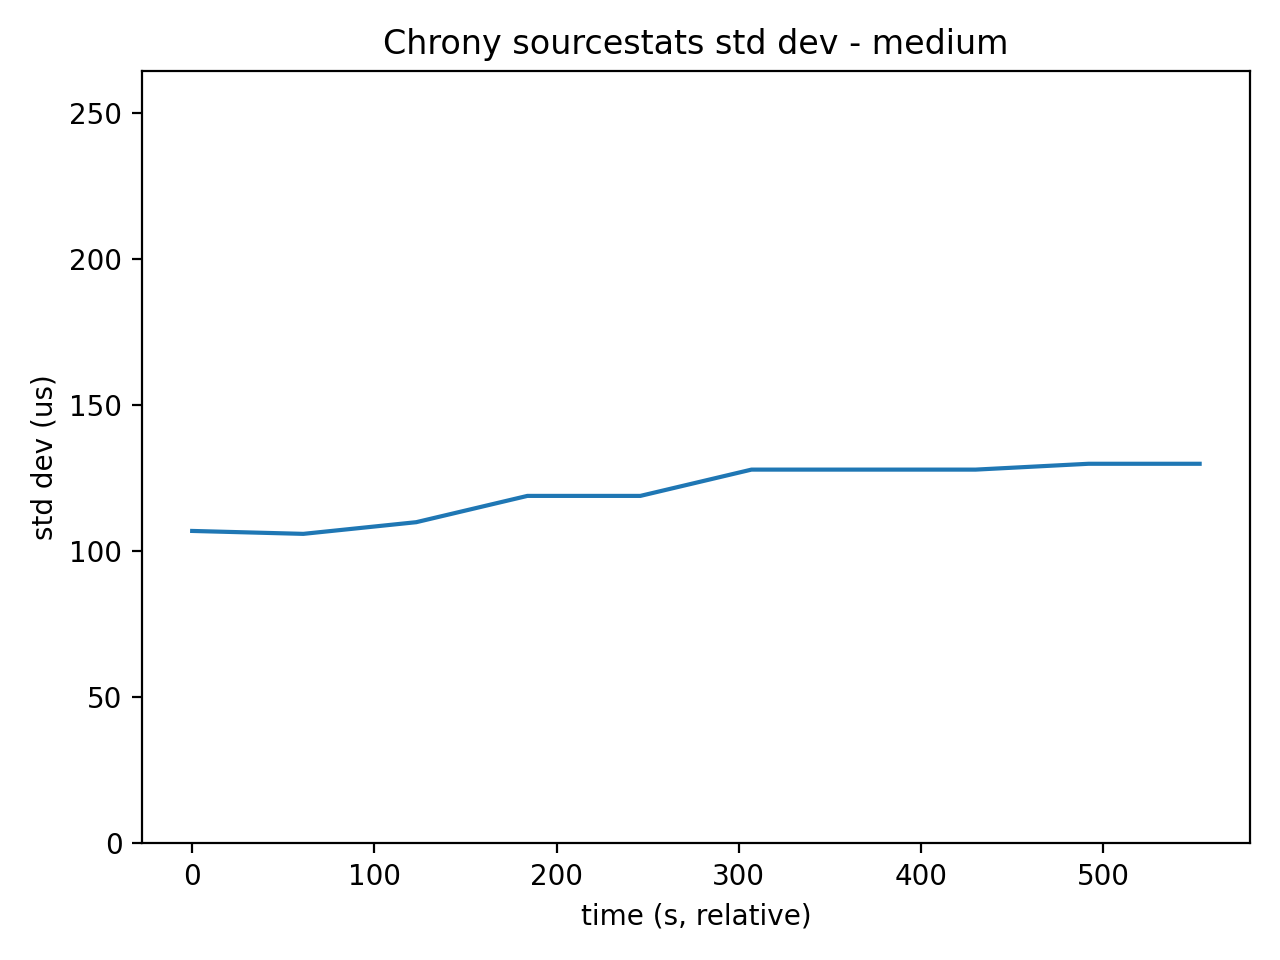
\includegraphics[width=\linewidth]{
      images/data_plots/plots_chrony_servergm/chrony_medium_sourcestats_stddev_us.png
    }
    \caption{Scenario MEDIUM}
  \end{subfigure}
  \begin{subfigure}
    {0.32\textwidth}
    \centering
    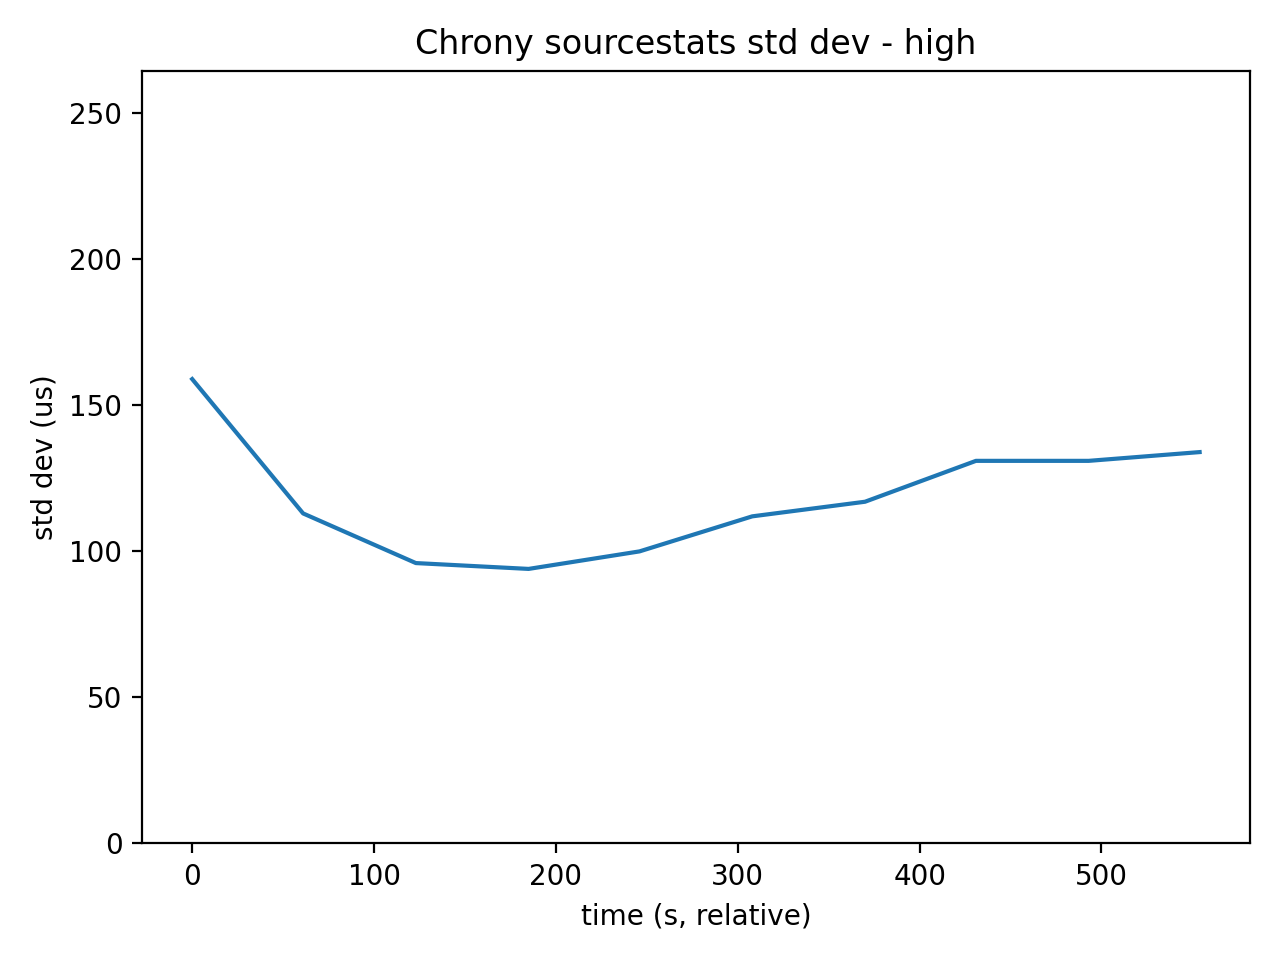
\includegraphics[width=\linewidth]{
      images/data_plots/plots_chrony_servergm/chrony_high_sourcestats_stddev_us.png
    }
    \caption{Scenario HIGH}
  \end{subfigure}
  \caption{Comparazione della performance - nodo: \texttt{clientchrony} - netem/tc:
  \texttt{servergm}}
  \label{fig:scenario_comparison}
\end{figure}
\paragraph*{clientchrony - netem/tc:}
L’analisi della metrica \texttt{std dev} restituita da \texttt{chronyc
sourcestats} mostra un comportamento complessivamente stabile tra i tre scenari, pur
in presenza di oscillazioni locali dovute al numero limitato di campioni disponibili.
Nello scenario \texttt{low} si osservano valori compresi tra 45~$\mu s$ e 171~$\mu
s$, con media pari a 110~$\mu s$ e mediana pari a 113.5~$\mu s$. Lo scenario \texttt{medium}
presenta valori centrali molto simili, con media pari a 111.2~$\mu s$ e mediana pari
a 109~$\mu s$, ma con una dispersione più elevata, evidenziata sia dal massimo di
218~$\mu s$ sia dalla deviazione standard pari a 55.98~$\mu s$. Nello scenario
\texttt{high}, invece, il livello centrale risulta leggermente più alto, con
media pari a 135.8~$\mu s$ e mediana pari a 131.5~$\mu s$, mentre la variabilità relativa
è più contenuta rispetto agli altri casi, come indicato dal coefficiente di
variazione pari a 0.219.

Dal punto di vista grafico non emerge un andamento monotono o una crescita netta
e sistematica della metrica al crescere dello stress di rete applicato sul nodo
\texttt{clientchrony}. Le differenze tra \texttt{low} e \texttt{medium}
risultano infatti trascurabili nei valori centrali, mentre lo scenario \texttt{high}
mostra un moderato incremento del livello medio della deviazione standard, senza però
evidenziare una discontinuità marcata rispetto agli altri due casi. In termini
oggettivi, i dati non indicano un effetto forte e chiaramente strutturale delle condizioni
di rete su questa metrica, ma soltanto una lieve tendenza a valori più elevati
nello scenario di stress massimo.

\paragraph*{servergm - netem/tc:}
L’analisi della metrica \texttt{std dev} con \texttt{netem/tc} applicato sul nodo
\texttt{servergm} evidenzia differenze più marcate tra i tre scenari rispetto a
quanto osservato nel caso di applicazione sul \texttt{clientchrony}. Nello
scenario \texttt{low} la deviazione standard assume i valori più elevati dell’intera
serie, con media pari a 214.9~$\mu s$, mediana pari a 217.5~$\mu s$ e valori compresi
tra 170~$\mu s$ e 252~$\mu s$. Il profilo temporale mostra inoltre un andamento
prevalentemente crescente, con oscillazioni limitate ma su livelli sistematicamente
alti.

Nello scenario \texttt{medium} si osserva invece una netta riduzione del livello
centrale, con media pari a 120.5~$\mu s$ e mediana pari a 123.5~$\mu s$. Anche
la dispersione risulta più contenuta, come indicato dalla deviazione standard pari
a 9.76~$\mu s$ e dall’intervallo complessivo di 24~$\mu s$. I valori si
mantengono quindi concentrati in una fascia relativamente stretta.

Lo scenario \texttt{high} presenta un comportamento molto simile al caso \texttt{medium},
con media pari a 118.7~$\mu s$ e mediana pari a 115~$\mu s$. La variabilità
resta moderata, con minimo pari a 94~$\mu s$ e massimo pari a 159~$\mu s$, senza
evidenziare incrementi sistematici rispetto allo scenario intermedio.

Nel complesso, i dati non mostrano una crescita monotona della metrica al crescere
dello stress di rete. Al contrario, lo scenario \texttt{low} risulta quello con
i valori di \texttt{std dev} più elevati, mentre gli scenari \texttt{medium} e \texttt{high}
si collocano su livelli sensibilmente inferiori e tra loro piuttosto vicini. In termini
oggettivi, l’effetto osservato non è quindi coerente con una dipendenza diretta
e progressiva dalle condizioni di rete imposte nei tre scenari.

\paragraph*{Confronto:}
Il confronto tra i due casi di applicazione di \texttt{netem} mostra una
differenza abbastanza netta nel comportamento della metrica \texttt{std dev}.
Quando il degrado è applicato sul \texttt{clientchrony}, i valori osservati si
collocano su livelli medi inferiori negli scenari \texttt{low} e \texttt{medium},
con medie pari rispettivamente a 110.0~$\mu s$ e 111.2~$\mu s$, mentre nello
scenario \texttt{high} si osserva un incremento moderato fino a 135.8~$\mu s$.
In questo caso, quindi, la metrica resta complessivamente contenuta, pur con una certa
irregolarità temporale.

Quando invece \texttt{netem} è applicato sul \texttt{servergm}, il comportamento
risulta diverso. Lo scenario \texttt{low} presenta infatti valori molto più
elevati, con media pari a 214.9~$\mu s$ e mediana pari a 217.5~$\mu s$,
nettamente superiori a quelli ottenuti nel caso di degrado sul client. Negli scenari
\texttt{medium} e \texttt{high}, invece, i livelli si riducono sensibilmente e tornano
vicini a quelli misurati con \texttt{netem} sul \texttt{clientchrony}, con medie
pari rispettivamente a 120.5~$\mu s$ e 118.7~$\mu s$.

Dal confronto diretto emerge quindi che la differenza principale tra i due
contesti non riguarda tanto gli scenari \texttt{medium} e \texttt{high}, che mostrano
valori abbastanza simili, quanto piuttosto lo scenario \texttt{low}, nel quale
il degrado applicato sul \texttt{servergm} produce una deviazione standard molto più
elevata rispetto al degrado applicato sul \texttt{clientchrony}. In termini strettamente
descrittivi, non si osserva dunque una relazione monotona e uniforme né rispetto
all’intensità dello stress né rispetto al nodo su cui esso viene introdotto; si rileva
piuttosto una forte sensibilità del caso \texttt{low} con \texttt{netem} applicato
sul lato \texttt{servergm}, mentre negli altri scenari i due assetti forniscono risultati
complessivamente più vicini.

\subsection{Analisi metrica: \texttt{system time offset}}
\begin{figure}[H]
  \centering

  \begin{subfigure}
    {0.32\textwidth}
    \centering
    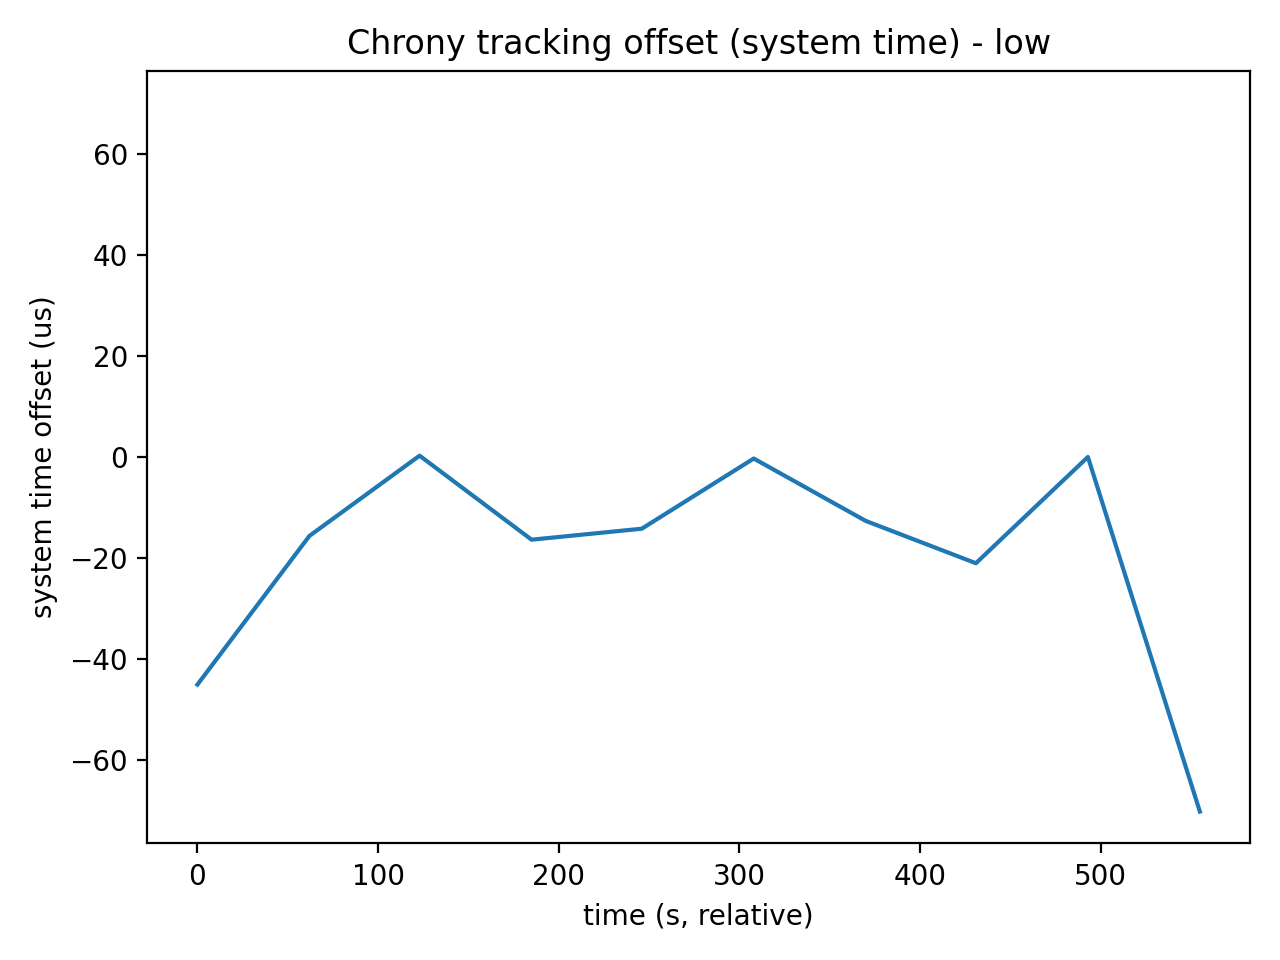
\includegraphics[width=\linewidth]{
      images/data_plots/plots_chrony_clientchrony/chrony_low_tracking_system_time_offset_us.png
    }
    \caption{Scenario LOW}
  \end{subfigure}
  \hfill
  \begin{subfigure}
    {0.32\textwidth}
    \centering
    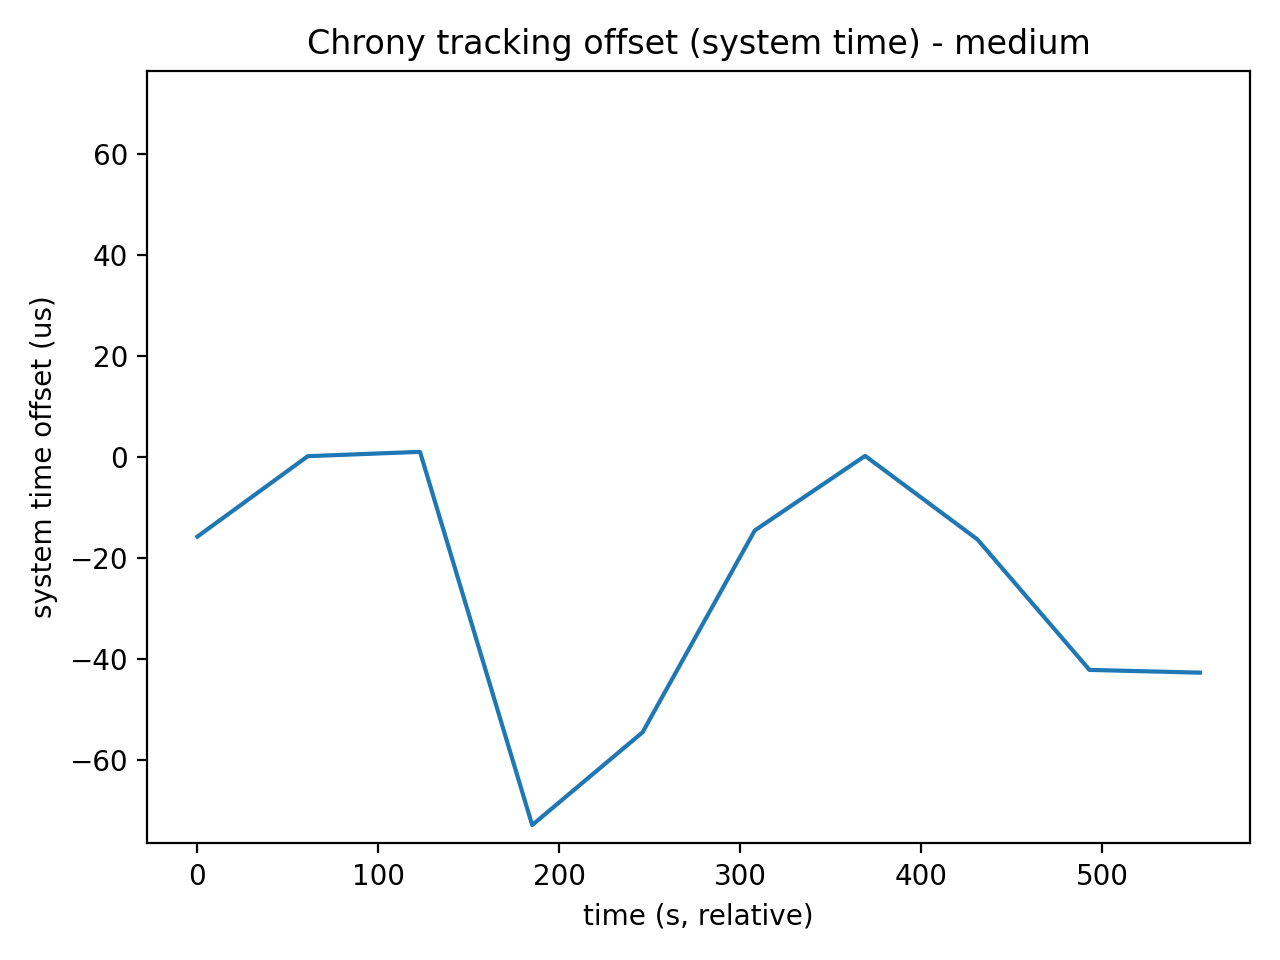
\includegraphics[width=\linewidth]{
      images/data_plots/plots_chrony_clientchrony/chrony_medium_tracking_system_time_offset_us.png
    }
    \caption{Scenario MEDIUM}
  \end{subfigure}
  \begin{subfigure}
    {0.32\textwidth}
    \centering
    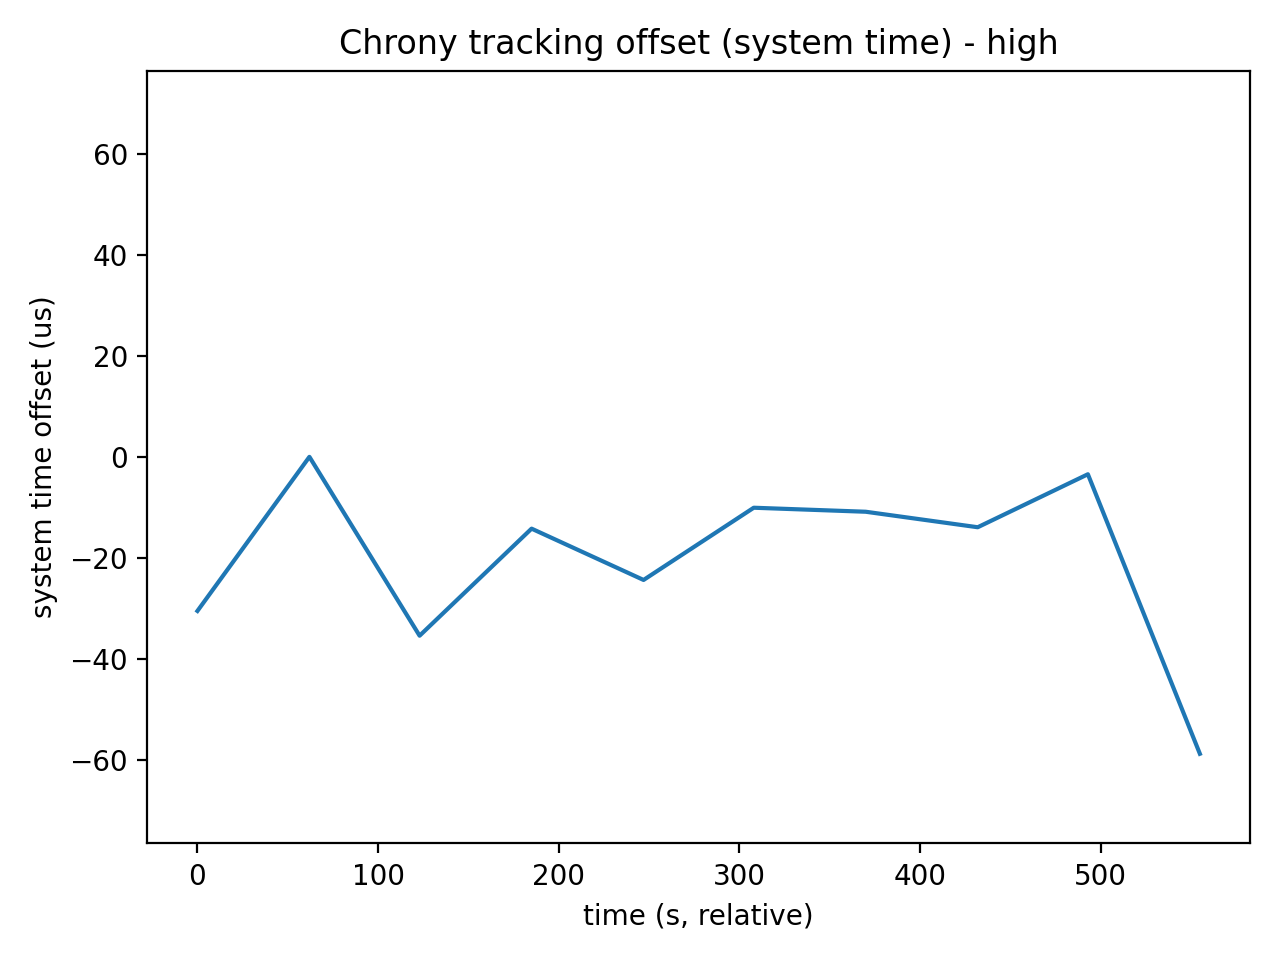
\includegraphics[width=\linewidth]{
      images/data_plots/plots_chrony_clientchrony/chrony_high_tracking_system_time_offset_us.png
    }
    \caption{Scenario HIGH}
  \end{subfigure}
  \caption{Comparazione della performance - nodo: \texttt{clientchrony} - netem/tc:
  \texttt{clientchrony}}
  \label{fig:scenario_comparison}
\end{figure}
\begin{figure}[H]
  \centering

  \begin{subfigure}
    {0.32\textwidth}
    \centering
    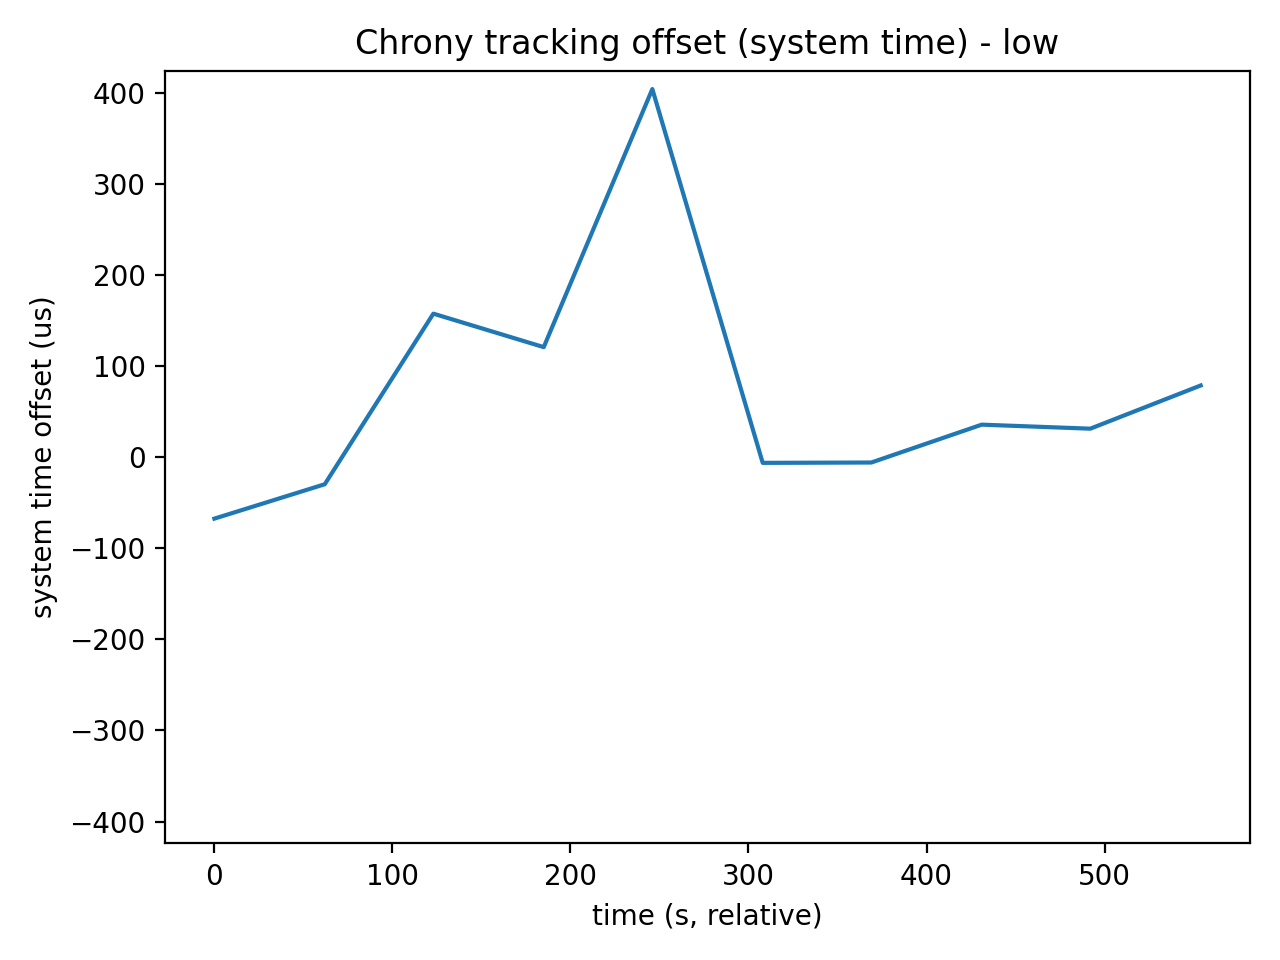
\includegraphics[width=\linewidth]{
      images/data_plots/plots_chrony_servergm/chrony_low_tracking_system_time_offset_us.png
    }
    \caption{Scenario LOW}
  \end{subfigure}
  \hfill
  \begin{subfigure}
    {0.32\textwidth}
    \centering
    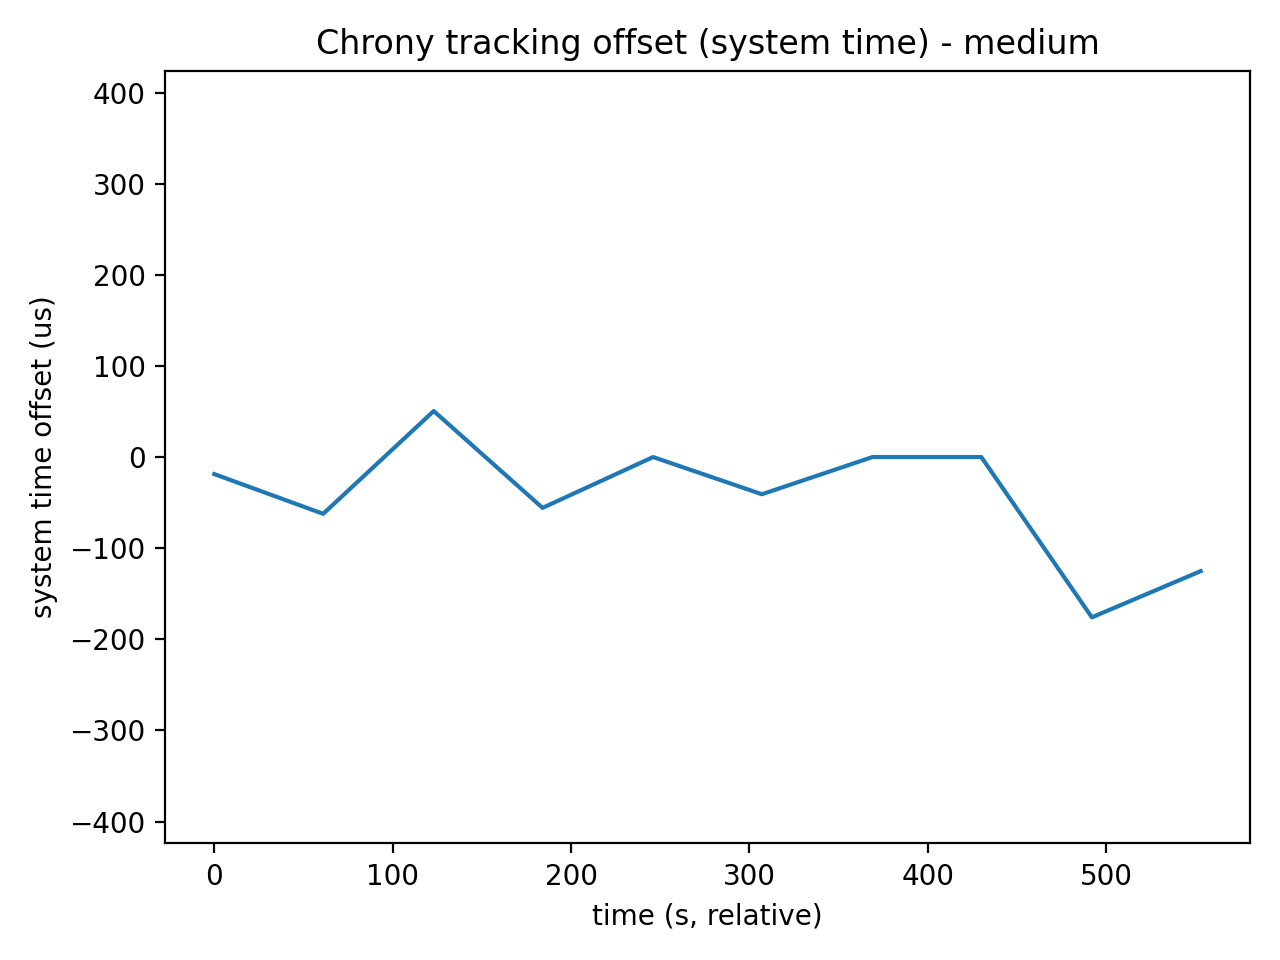
\includegraphics[width=\linewidth]{
      images/data_plots/plots_chrony_servergm/chrony_medium_tracking_system_time_offset_us.png
    }
    \caption{Scenario MEDIUM}
  \end{subfigure}
  \begin{subfigure}
    {0.32\textwidth}
    \centering
    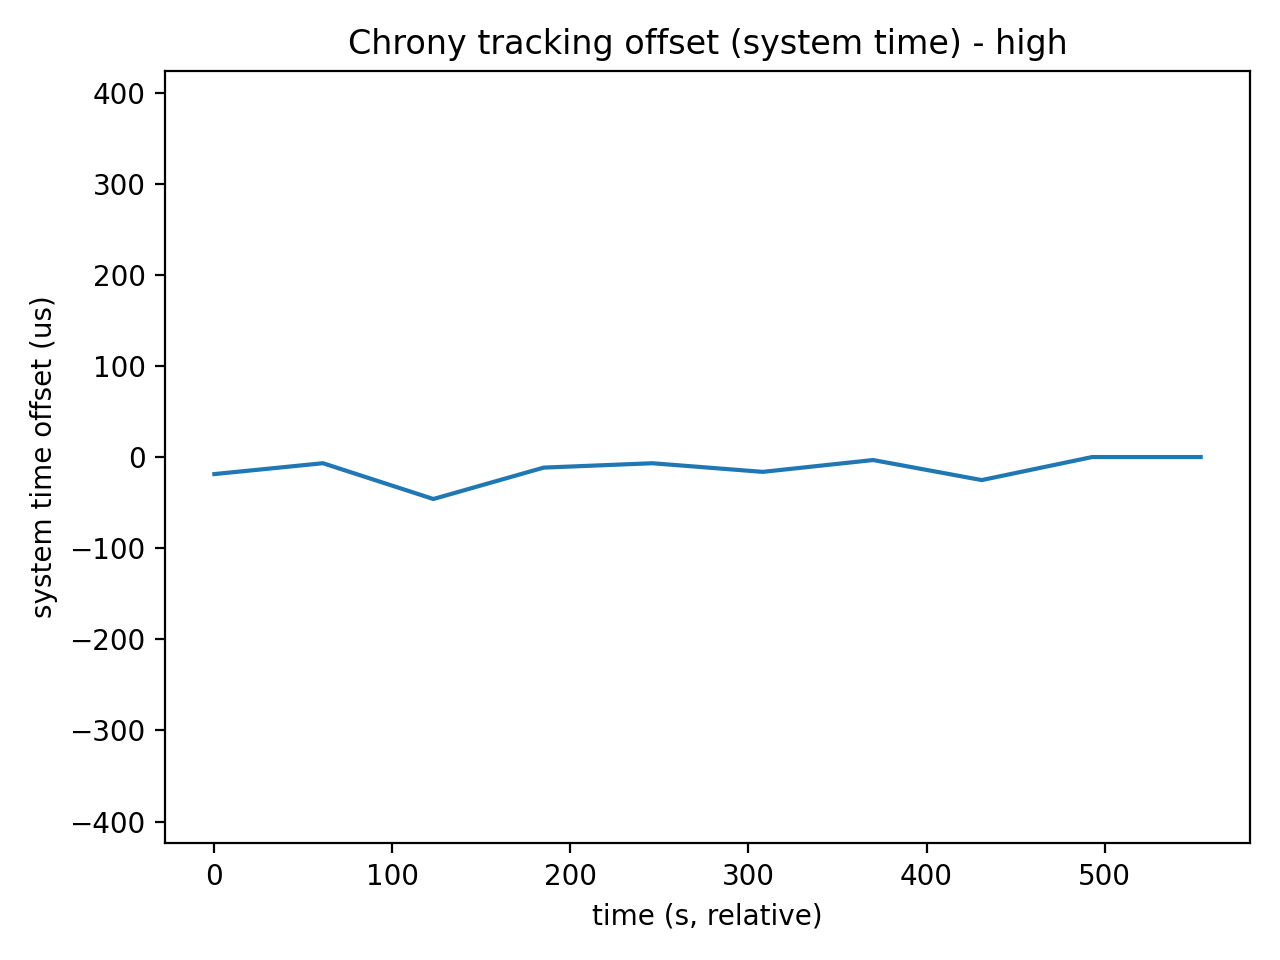
\includegraphics[width=\linewidth]{
      images/data_plots/plots_chrony_servergm/chrony_high_tracking_system_time_offset_us.png
    }
    \caption{Scenario HIGH}
  \end{subfigure}
  \caption{Comparazione della performance - nodo: \texttt{clientchrony} - netem/tc:
  \texttt{servergm}}
  \label{fig:scenario_comparison}
\end{figure}
\paragraph*{clientchrony - netem/tc:}
L’analisi del \texttt{system time offset} del nodo \texttt{clientchrony}, nel caso
in cui il \texttt{netem/tc} sia applicato sul client stesso, mostra valori sempre
contenuti nell’ordine dei microsecondi ($\mu s$), senza evidenziare una
separazione netta e sistematica tra i tre scenari di carico.

Nel caso \texttt{low}, la serie presenta un andamento prevalentemente negativo, con
media pari a $-19.5298~\mu s$ e mediana pari a $-14.9195~\mu s$; si osservano
tuttavia alcune misure prossime allo zero e un minimo pari a $-70.277~\mu s$. Lo scenario
\texttt{medium} mostra il valore medio più negativo, pari a $-25.7615~\mu s$,
una mediana di $-16.0345~\mu s$ e anche la maggiore dispersione, con deviazione standard
pari a $25.8088~\mu s$ e intervallo interquartile di $39.09075~\mu s$. Nel caso
\texttt{high}, invece, i valori risultano leggermente più concentrati: la media
è pari a $-20.1462~\mu s$, la mediana a $-14.052~\mu s$ e la deviazione standard scende
a $17.6532~\mu s$.

Dal punto di vista grafico, tutti e tre gli scenari mostrano oscillazioni
moderate attorno a valori negativi, con alcuni campioni isolati vicini allo zero e
senza un andamento progressivamente peggiorativo all’aumentare dello stress di rete.
Anche i valori estremi, pur presenti in ciascuno scenario, non delineano una
progressione monotona: il minimo più marcato compare nel caso \texttt{medium} ($-
72.943~\mu s$), mentre lo scenario \texttt{high} non risulta il più penalizzato.

Nel complesso, per questa metrica non emerge una differenza strutturale chiaramente
attribuibile alle diverse condizioni di rete applicate sul \texttt{clientchrony}.
Le variazioni osservate indicano una certa fluttuazione tra scenari, ma non
supportano l’ipotesi di un deterioramento sistematico del \texttt{system time
offset} al crescere del livello di stress.

\paragraph*{servergm - netem/tc:}
L’analisi del \texttt{system time offset} del nodo \texttt{clientchrony}, nel caso
in cui il degrado di rete sia applicato sul nodo \texttt{servergm}, evidenzia un comportamento
differenziato tra i tre scenari, con variazioni più marcate rispetto a quanto
osservato per altre metriche.

Nel caso \texttt{low}, la serie assume valori mediamente positivi, con media pari
a $71.7357~\mu s$ e mediana pari a $33.3505~\mu s$. La dispersione è elevata, come
indicato dalla deviazione standard di $135.3627~\mu s$, e il profilo temporale
mostra un picco massimo di $403.865~\mu s$, che contribuisce in modo rilevante ad
aumentare il valore medio.

Lo scenario \texttt{medium} presenta invece un livello centrale negativo, con media
pari a $-42.8227~\mu s$ e mediana pari a $-29.7855~\mu s$. Anche in questo caso
la variabilità rimane significativa, con deviazione standard di $66.5330~\mu s$ e
minimo pari a $-175.907~\mu s$. La serie oscilla attorno a valori negativi, con alcuni
campioni prossimi allo zero ma senza stabilizzarsi su livelli positivi.

Nel caso \texttt{high}, il \texttt{system time offset} risulta il più contenuto
dei tre scenari. La media è pari a $-13.4635~\mu s$, la mediana a $-9.183~\mu s$
e la deviazione standard scende a $14.1233~\mu s$, nettamente inferiore rispetto ai
casi \texttt{low} e \texttt{medium}. Anche il campo di variazione si riduce
sensibilmente, con valori compresi tra $-46.044~\mu s$ e $0.007~\mu s$.

Nel complesso, i dati non mostrano un peggioramento monotono del \texttt{system
time offset} all’aumentare dello stress di rete applicato sul \texttt{servergm}. Al
contrario, lo scenario \texttt{low} è quello che presenta gli scostamenti positivi
più elevati e la maggiore variabilità complessiva, mentre lo scenario \texttt{high}
appare il più stabile e contenuto. Pertanto, anche in questo caso non emerge una relazione
lineare e sistematica tra intensità del carico di rete e deterioramento della metrica.

\paragraph*{Confronto:}
Il confronto tra i due casi di applicazione di \texttt{netem/tc} per la metrica \texttt{system
time offset} mette in evidenza differenze più nette rispetto a quanto osservato
per \texttt{offset} e \texttt{std dev}.

Quando il degrado è applicato su \texttt{clientchrony}, i tre scenari mantengono
valori medi sempre negativi e relativamente contenuti: la media passa da $-19.529
8~\mu s$ nel caso \texttt{low}, a $-25.7615~\mu s$ nel caso \texttt{medium}, fino
a $-20.1462~\mu s$ nel caso \texttt{high}. Anche le mediane restano vicine tra loro,
comprese tra circa $-16~\mu s$ e $-14~\mu s$, mentre la dispersione è moderata,
pur con alcune escursioni più marcate nei casi \texttt{low} e \texttt{medium}. Nel
complesso, il comportamento risulta piuttosto stabile e non emerge una
differenza strutturale chiara tra i tre livelli di stress.

Diversamente, quando il degrado è applicato su \texttt{servergm}, la metrica mostra
una sensibilità maggiore alla collocazione del disturbo. In questo caso lo
scenario \texttt{low} presenta valori medi positivi, con media pari a
$71.7357~\mu s$ e un picco massimo di $403.865~\mu s$, risultando nettamente più instabile
degli altri. Lo scenario \texttt{medium} si sposta invece su valori medi negativi,
con media pari a $-42.8227~\mu s$, mentre il caso \texttt{high} torna a un
comportamento più contenuto, con media pari a $-13.4635~\mu s$ e la minore deviazione
standard tra i tre scenari.

Il confronto diretto mostra quindi che l’applicazione del degrado su \texttt{servergm}
produce effetti più marcati e irregolari sul \texttt{system time offset},
soprattutto nei casi \texttt{low} e \texttt{medium}, mentre l’applicazione su \texttt{clientchrony}
conduce a valori più contenuti e complessivamente più omogenei. Anche considerando
entrambi i contesti, non si osserva comunque una crescita monotona del
disallineamento al crescere dello stress di rete: la differenza principale riguarda
piuttosto la maggiore instabilità introdotta quando il degrado interessa il lato \texttt{servergm}.